%&preformat-disser
\RequirePackage[l2tabu,orthodox]{nag} % Раскомментировав, можно в логе получать рекомендации относительно правильного использования пакетов и предупреждения об устаревших и нерекомендуемых пакетах
% Формат А4, 14pt (ГОСТ Р 7.0.11-2011, 5.3.6)
\documentclass[a4paper,14pt,oneside,openany]{memoir}

%%%%%%%%%%%%%%%%%%%%%%%%%%%%%%%%%%%%%%%%%%%%%%%%%%%%%%%%%%%%%%%%%%%%%%%%%%%%%%%%
%%%% Файл упрощённых настроек шаблона, общих для диссертации и автореферата %%%%
%%%%%%%%%%%%%%%%%%%%%%%%%%%%%%%%%%%%%%%%%%%%%%%%%%%%%%%%%%%%%%%%%%%%%%%%%%%%%%%%

%%% Режим черновика %%%
\makeatletter
\@ifundefined{c@draft}{
  \newcounter{draft}
  \setcounter{draft}{0}  % 0 --- чистовик (максимальное соблюдение ГОСТ)
                         % 1 --- черновик (отклонения от ГОСТ, но быстрая
                         %       сборка итоговых PDF)
}{}
\makeatother

%%% Пометки в тексте %%%
\makeatletter
\@ifundefined{c@showmarkup}{
  \newcounter{showmarkup}
  \setcounter{showmarkup}{0}  % 0 --- скрыть пометки
                              % 1 --- показывать пометки
}{}
\makeatother

%%% Использование в pdflatex шрифтов не по-умолчанию %%%
\makeatletter
\@ifundefined{c@usealtfont}{
  \newcounter{usealtfont}
  \setcounter{usealtfont}{1}    % 0 --- шрифты на базе Computer Modern
                                % 1 --- использовать пакет pscyr, при его
                                %       наличии
                                % 2 --- использовать пакет XCharter, при наличии
                                %       подходящей версии
}{}
\makeatother

%%% Использование в xelatex и lualatex семейств шрифтов %%%
\makeatletter
\@ifundefined{c@fontfamily}{
  \newcounter{fontfamily}
  \setcounter{fontfamily}{1}  % 0 --- CMU семейство. Используется как fallback;
                              % 1 --- Шрифты от MS (Times New Roman и компания)
                              % 2 --- Семейство Liberation
}{}
\makeatother

%%% Библиография %%%
\makeatletter
\@ifundefined{c@bibliosel}{
  \newcounter{bibliosel}
  \setcounter{bibliosel}{0}   % 0 --- встроенная реализация с загрузкой файла
                              %       через движок bibtex8;
                              % 1 --- реализация пакетом biblatex через движок
                              %       biber
}{}
\makeatother

%%% Вывод типов ссылок в библиографии %%%
\makeatletter
\@ifundefined{c@mediadisplay}{
  \newcounter{mediadisplay}
  \setcounter{mediadisplay}{1}   % 0 --- не делать ничего; надписи [Текст] и
                                 %       [Эл. ресурс] будут выводиться только в ссылках с
                                 %       заполненным полем `media`;
                                 % 1 --- автоматически добавлять надпись [Текст] к ссылкам с
                                 %       незаполненным полем `media`; таким образом, у всех
                                 %       источников будет указан тип, что соответствует
                                 %       требованиям ГОСТ
                                 % 2 --- автоматически удалять надписи [Текст], [Эл. Ресурс] и др.;
                                 %       не соответствует ГОСТ
                                 % 3 --- автоматически удалять надпись [Текст];
                                 %       не соответствует ГОСТ
                                 % 4 --- автоматически удалять надпись [Эл. Ресурс];
                                 %       не соответствует ГОСТ
}{}
\makeatother

%%% Предкомпиляция tikz рисунков для ускорения работы %%%
\makeatletter
\@ifundefined{c@imgprecompile}{
  \newcounter{imgprecompile}
  \setcounter{imgprecompile}{0}   % 0 --- без предкомпиляции;
                                  % 1 --- пользоваться предварительно
                                  %       скомпилированными pdf вместо генерации
                                  %       заново из tikz
}{}
\makeatother
            % общие настройки шаблона
\input{common/packages}         % Пакеты общие для диссертации и автореферата
\synopsisfalse                      % Этот документ --- не автореферат
\input{Dissertation/dispackages}    % Пакеты для диссертации
\usepackage{fr-longtable}    %ради \endlasthead

% Листинги с исходным кодом программ
\usepackage{fancyvrb}
\usepackage{listings}
\lccode`\~=0\relax %Без этого хака из-за особенностей пакета listings перестают работать конструкции с \MakeLowercase и т. п. в (xe|lua)latex

% Русская традиция начертания греческих букв
\usepackage{upgreek} % прямые греческие ради русской традиции

%%% Микротипографика
\ifnumequal{\value{draft}}{0}{% Только если у нас режим чистовика
    \usepackage[final, babel, shrink=45]{microtype}[2016/05/14] % улучшает представление букв и слов в строках, может помочь при наличии отдельно висящих слов
}{}

% Отметка о версии черновика на каждой странице
% Чтобы работало надо в своей локальной копии по инструкции
% https://www.ctan.org/pkg/gitinfo2 создать небходимые файлы в папке
% ./git/hooks
% If you’re familiar with tweaking git, you can probably work it out for
% yourself. If not, I suggest you follow these steps:
% 1. First, you need a git repository and working tree. For this example,
% let’s suppose that the root of the working tree is in ~/compsci
% 2. Copy the file post-xxx-sample.txt (which is in the same folder of
% your TEX distribution as this pdf) into the git hooks directory in your
% working copy. In our example case, you should end up with a file called
% ~/compsci/.git/hooks/post-checkout
% 3. If you’re using a unix-like system, don’t forget to make the file executable.
% Just how you do this is outside the scope of this manual, but one
% possible way is with commands such as this:
% chmod g+x post-checkout.
% 4. Test your setup with “git checkout master” (or another suitable branch
% name). This should generate copies of gitHeadInfo.gin in the directories
% you intended.
% 5. Now make two more copies of this file in the same directory (hooks),
% calling them post-commit and post-merge, and you’re done. As before,
% users of unix-like systems should ensure these files are marked as
% executable.
\ifnumequal{\value{draft}}{1}{% Черновик
   \IfFileExists{.git/gitHeadInfo.gin}{
      \usepackage[mark,pcount]{gitinfo2}
      \renewcommand{\gitMark}{rev.\gitAbbrevHash\quad\gitCommitterEmail\quad\gitAuthorIsoDate}
      \renewcommand{\gitMarkFormat}{\rmfamily\color{Gray}\small\bfseries}
   }{}
}{}   % Пакеты для специфических пользовательских задач

%%%%%%%%%%%%%%%%%%%%%%%%%%%%%%%%%%%%%%%%%%%%%%%%%%%%%%%%%%%%%%%%%%%%%%%%%%%%%%%%
%%%% Файл упрощённых настроек шаблона, общих для диссертации и автореферата %%%%
%%%%%%%%%%%%%%%%%%%%%%%%%%%%%%%%%%%%%%%%%%%%%%%%%%%%%%%%%%%%%%%%%%%%%%%%%%%%%%%%

%%% Режим черновика %%%
\makeatletter
\@ifundefined{c@draft}{
  \newcounter{draft}
  \setcounter{draft}{0}  % 0 --- чистовик (максимальное соблюдение ГОСТ)
                         % 1 --- черновик (отклонения от ГОСТ, но быстрая
                         %       сборка итоговых PDF)
}{}
\makeatother

%%% Пометки в тексте %%%
\makeatletter
\@ifundefined{c@showmarkup}{
  \newcounter{showmarkup}
  \setcounter{showmarkup}{0}  % 0 --- скрыть пометки
                              % 1 --- показывать пометки
}{}
\makeatother

%%% Использование в pdflatex шрифтов не по-умолчанию %%%
\makeatletter
\@ifundefined{c@usealtfont}{
  \newcounter{usealtfont}
  \setcounter{usealtfont}{1}    % 0 --- шрифты на базе Computer Modern
                                % 1 --- использовать пакет pscyr, при его
                                %       наличии
                                % 2 --- использовать пакет XCharter, при наличии
                                %       подходящей версии
}{}
\makeatother

%%% Использование в xelatex и lualatex семейств шрифтов %%%
\makeatletter
\@ifundefined{c@fontfamily}{
  \newcounter{fontfamily}
  \setcounter{fontfamily}{1}  % 0 --- CMU семейство. Используется как fallback;
                              % 1 --- Шрифты от MS (Times New Roman и компания)
                              % 2 --- Семейство Liberation
}{}
\makeatother

%%% Библиография %%%
\makeatletter
\@ifundefined{c@bibliosel}{
  \newcounter{bibliosel}
  \setcounter{bibliosel}{0}   % 0 --- встроенная реализация с загрузкой файла
                              %       через движок bibtex8;
                              % 1 --- реализация пакетом biblatex через движок
                              %       biber
}{}
\makeatother

%%% Вывод типов ссылок в библиографии %%%
\makeatletter
\@ifundefined{c@mediadisplay}{
  \newcounter{mediadisplay}
  \setcounter{mediadisplay}{1}   % 0 --- не делать ничего; надписи [Текст] и
                                 %       [Эл. ресурс] будут выводиться только в ссылках с
                                 %       заполненным полем `media`;
                                 % 1 --- автоматически добавлять надпись [Текст] к ссылкам с
                                 %       незаполненным полем `media`; таким образом, у всех
                                 %       источников будет указан тип, что соответствует
                                 %       требованиям ГОСТ
                                 % 2 --- автоматически удалять надписи [Текст], [Эл. Ресурс] и др.;
                                 %       не соответствует ГОСТ
                                 % 3 --- автоматически удалять надпись [Текст];
                                 %       не соответствует ГОСТ
                                 % 4 --- автоматически удалять надпись [Эл. Ресурс];
                                 %       не соответствует ГОСТ
}{}
\makeatother

%%% Предкомпиляция tikz рисунков для ускорения работы %%%
\makeatletter
\@ifundefined{c@imgprecompile}{
  \newcounter{imgprecompile}
  \setcounter{imgprecompile}{0}   % 0 --- без предкомпиляции;
                                  % 1 --- пользоваться предварительно
                                  %       скомпилированными pdf вместо генерации
                                  %       заново из tikz
}{}
\makeatother
      % Упрощённые настройки шаблона

% Новые переменные, которые могут использоваться во всём проекте
% ГОСТ 7.0.11-2011
% 9.2 Оформление текста автореферата диссертации
% 9.2.1 Общая характеристика работы включает в себя следующие основные структурные
% элементы:
% актуальность темы исследования;
\newcommand{\actualityTXT}{Актуальность темы исследования.}
% степень ее разработанности;
\newcommand{\progressTXT}{Степень разработанности темы исследования.}
% цели и задачи;
\newcommand{\aimTXT}{Целью}
\newcommand{\tasksTXT}{задачи}
% научную новизну;
\newcommand{\noveltyTXT}{Научная новизна.}
% теоретическую и практическую значимость работы;
%\newcommand{\influenceTXT}{Теоретическая и практическая значимость}
% или чаще используют просто
\newcommand{\thInfluenceTXT}{Теоретическая значимость.}
\newcommand{\prInfluenceTXT}{Практическая значимость.}
% методологию и методы исследования;
\newcommand{\methodsTXT}{Методология и методы исследования.}
% положения, выносимые на защиту;
\newcommand{\defpositionsTXT}{Основные положения, выносимые на~защиту:}
% степень достоверности и апробацию результатов.
\newcommand{\reliabilityTXT}{Достоверность}
\newcommand{\probationTXT}{Апробация работы.}

\newcommand{\contributionTXT}{Личный вклад.}
\newcommand{\publicationsTXT}{Публикации.}


%%% Заголовки библиографии:

% для автореферата:
\newcommand{\bibtitleauthor}{Публикации автора по теме диссертации}

% для стиля библиографии `\insertbiblioauthorgrouped`
\newcommand{\bibtitleauthorvak}{В изданиях из списка ВАК РФ}
\newcommand{\bibtitleauthorscopus}{В изданиях, входящих в международную базу цитирования Scopus}
\newcommand{\bibtitleauthorwos}{В изданиях, входящих в международную базу цитирования Web of Science}
\newcommand{\bibtitleauthorother}{В прочих изданиях}
\newcommand{\bibtitleauthorconf}{В сборниках трудов конференций}
\newcommand{\bibtitleauthorpatent}{Зарегистрированные патенты}
\newcommand{\bibtitleauthorprogram}{Зарегистрированные программы для ЭВМ}

% для стиля библиографии `\insertbiblioauthorimportant`:
\newcommand{\bibtitleauthorimportant}{Наиболее значимые \protect\MakeLowercase\bibtitleauthor}

% для списка литературы в диссертации и списка чужих работ в автореферате:
\newcommand{\bibtitlefull}{Список литературы} % (ГОСТ Р 7.0.11-2011, 4)
         % Новые переменные, для всего проекта

%%% Основные сведения %%%
\newcommand{\thesisAuthorLastName}{Булатов}
\newcommand{\thesisAuthorOtherNames}{Виктор Геннадьевич}
\newcommand{\thesisAuthorInitials}{В.\,Г.}
\newcommand{\thesisAuthor}             % Диссертация, ФИО автора
{%
    \texorpdfstring{% \texorpdfstring takes two arguments and uses the first for (La)TeX and the second for pdf
        \thesisAuthorLastName~\thesisAuthorOtherNames% так будет отображаться на титульном листе или в тексте, где будет использоваться переменная
    }{%
        \thesisAuthorLastName, \thesisAuthorOtherNames% эта запись для свойств pdf-файла. В таком виде, если pdf будет обработан программами для сбора библиографических сведений, будет правильно представлена фамилия.
    }
}
\newcommand{\thesisAuthorShort}        % Диссертация, ФИО автора инициалами
{\thesisAuthorInitials~\thesisAuthorLastName}
%\newcommand{\thesisUdk}                % Диссертация, УДК
%{\fixme{xxx.xxx}}
\newcommand{\thesisTitle}              % Диссертация, название
{Методы оценивания качества  и многокритериальной оптимизации тематических моделей в библиотеке TopicNet}
\newcommand{\thesisSpecialtyNumber}    % Диссертация, специальность, номер
{05.13.18}
\newcommand{\thesisSpecialtyTitle}     % Диссертация, специальность, название (название взято с сайта ВАК для примера)
{Математическое моделирование, численные методы и комплексы программ}
\newcommand{\thesisDegree}             % Диссертация, ученая степень
{кандидата технических наук}
\newcommand{\thesisDegreeShort}        % Диссертация, ученая степень, краткая запись
{канд. техн. наук}
\newcommand{\thesisCity}               % Диссертация, город написания диссертации
{Москва}
\newcommand{\thesisYear}               % Диссертация, год написания диссертации
{\the\year}
\newcommand{\thesisOrganization}       % Диссертация, организация
{Федеральное государственное автономное образовательное учреждение высшего образования «Московский физико-технический институт (национальный исследовательский университет)»}
\newcommand{\thesisOrganizationShort}  % Диссертация, краткое название организации для доклада
{МФТИ (ГУ)}

\newcommand{\thesisInOrganization}     % Диссертация, организация в предложном падеже: Работа выполнена в ...
{\fixme{учреждении с~длинным длинным длинным длинным названием, в~котором
выполнялась данная диссертационная работа}}

%% \newcommand{\supervisorDead}{}           % Рисовать рамку вокруг фамилии
\newcommand{\supervisorFio}              % Научный руководитель, ФИО
{Воронцов Константин Вячеславович}
\newcommand{\supervisorRegalia}          % Научный руководитель, регалии
{доктор физико-математических наук}
\newcommand{\supervisorFioShort}         % Научный руководитель, ФИО
{К.\,В.~Воронцов}
\newcommand{\supervisorRegaliaShort}     % Научный руководитель, регалии
{д-р физ.-мат. наук}

%% \newcommand{\supervisorTwoDead}{}        % Рисовать рамку вокруг фамилии
%% \newcommand{\supervisorTwoFio}           % Второй научный руководитель, ФИО
%% {\fixme{Фамилия Имя Отчество}}
%% \newcommand{\supervisorTwoRegalia}       % Второй научный руководитель, регалии
%% {\fixme{уч. степень, уч. звание}}
%% \newcommand{\supervisorTwoFioShort}      % Второй научный руководитель, ФИО
%% {\fixme{И.\,О.~Фамилия}}
%% \newcommand{\supervisorTwoRegaliaShort}  % Второй научный руководитель, регалии
%% {\fixme{уч.~ст.,~уч.~зв.}}

\newcommand{\opponentOneFio}           % Оппонент 1, ФИО
{\fixme{Фамилия Имя Отчество}}
\newcommand{\opponentOneRegalia}       % Оппонент 1, регалии
{\fixme{доктор физико-математических наук, профессор}}
\newcommand{\opponentOneJobPlace}      % Оппонент 1, место работы
{\fixme{Не очень длинное название для места работы}}
\newcommand{\opponentOneJobPost}       % Оппонент 1, должность
{\fixme{старший научный сотрудник}}

\newcommand{\opponentTwoFio}           % Оппонент 2, ФИО
{\fixme{Фамилия Имя Отчество}}
\newcommand{\opponentTwoRegalia}       % Оппонент 2, регалии
{\fixme{кандидат физико-математических наук}}
\newcommand{\opponentTwoJobPlace}      % Оппонент 2, место работы
{\fixme{Основное место работы c длинным длинным длинным длинным названием}}
\newcommand{\opponentTwoJobPost}       % Оппонент 2, должность
{\fixme{старший научный сотрудник}}

%% \newcommand{\opponentThreeFio}         % Оппонент 3, ФИО
%% {\fixme{Фамилия Имя Отчество}}
%% \newcommand{\opponentThreeRegalia}     % Оппонент 3, регалии
%% {\fixme{кандидат физико-математических наук}}
%% \newcommand{\opponentThreeJobPlace}    % Оппонент 3, место работы
%% {\fixme{Основное место работы c длинным длинным длинным длинным названием}}
%% \newcommand{\opponentThreeJobPost}     % Оппонент 3, должность
%% {\fixme{старший научный сотрудник}}

\newcommand{\leadingOrganizationTitle} % Ведущая организация, дополнительные строки. Удалить, чтобы не отображать в автореферате
{\fixme{Федеральное государственное бюджетное образовательное учреждение высшего
профессионального образования с~длинным длинным длинным длинным названием}}

\newcommand{\defenseDate}              % Защита, дата
{\fixme{DD mmmmmmmm YYYY~г.~в~XX часов}}
\newcommand{\defenseCouncilNumber}     % Защита, номер диссертационного совета
{\fixme{Д\,123.456.78}}
\newcommand{\defenseCouncilTitle}      % Защита, учреждение диссертационного совета
{\fixme{Название учреждения}}
\newcommand{\defenseCouncilAddress}    % Защита, адрес учреждение диссертационного совета
{\fixme{Адрес}}
\newcommand{\defenseCouncilPhone}      % Телефон для справок
{\fixme{+7~(0000)~00-00-00}}

\newcommand{\defenseSecretaryFio}      % Секретарь диссертационного совета, ФИО
{\fixme{Фамилия Имя Отчество}}
\newcommand{\defenseSecretaryRegalia}  % Секретарь диссертационного совета, регалии
{\fixme{д-р~физ.-мат. наук}}            % Для сокращений есть ГОСТы, например: ГОСТ Р 7.0.12-2011 + http://base.garant.ru/179724/#block_30000

\newcommand{\synopsisLibrary}          % Автореферат, название библиотеки
{\fixme{Название библиотеки}}
\newcommand{\synopsisDate}             % Автореферат, дата рассылки
{\fixme{DD mmmmmmmm}\the\year~года}

% To avoid conflict with beamer class use \providecommand
\providecommand{\keywords}%            % Ключевые слова для метаданных PDF диссертации и автореферата
{}
             % Основные сведения
\input{common/fonts}            % Определение шрифтов (частичное)
%%% Шаблон %%%
\DeclareRobustCommand{\fixme}{\textcolor{red}}  % решаем проблему превращения
                                % названия цвета в результате \MakeUppercase,
                                % http://tex.stackexchange.com/a/187930,
                                % \DeclareRobustCommand protects \fixme
                                % from expanding inside \MakeUppercase
\AtBeginDocument{%
    \setlength{\parindent}{2.5em}                   % Абзацный отступ. Должен быть одинаковым по всему тексту и равен пяти знакам (ГОСТ Р 7.0.11-2011, 5.3.7).
}

%%% Таблицы %%%
\DeclareCaptionLabelSeparator{tabsep}{\tablabelsep} % нумерация таблиц
\DeclareCaptionFormat{split}{\splitformatlabel#1\par\splitformattext#3}

\captionsetup[table]{
        format=\tabformat,                % формат подписи (plain|hang)
        font=normal,                      % нормальные размер, цвет, стиль шрифта
        skip=.0pt,                        % отбивка под подписью
        parskip=.0pt,                     % отбивка между параграфами подписи
        position=above,                   % положение подписи
        justification=\tabjust,           % центровка
        indent=\tabindent,                % смещение строк после первой
        labelsep=tabsep,                  % разделитель
        singlelinecheck=\tabsinglecenter, % не выравнивать по центру, если умещается в одну строку
}

%%% Рисунки %%%
\DeclareCaptionLabelSeparator{figsep}{\figlabelsep} % нумерация рисунков

\captionsetup[figure]{
        format=plain,                     % формат подписи (plain|hang)
        font=normal,                      % нормальные размер, цвет, стиль шрифта
        skip=.0pt,                        % отбивка под подписью
        parskip=.0pt,                     % отбивка между параграфами подписи
        position=below,                   % положение подписи
        singlelinecheck=true,             % выравнивание по центру, если умещается в одну строку
        justification=centerlast,         % центровка
        labelsep=figsep,                  % разделитель
}

%%% Подписи подрисунков %%%
\DeclareCaptionSubType{figure}
\renewcommand\thesubfigure{\asbuk{subfigure}} % нумерация подрисунков
\ifsynopsis
\DeclareCaptionFont{norm}{\fontsize{10pt}{11pt}\selectfont}
\newcommand{\subfigureskip}{2.pt}
\else
\DeclareCaptionFont{norm}{\fontsize{14pt}{16pt}\selectfont}
\newcommand{\subfigureskip}{0.pt}
\fi

\captionsetup[subfloat]{
        labelfont=norm,                 % нормальный размер подписей подрисунков
        textfont=norm,                  % нормальный размер подписей подрисунков
        labelsep=space,                 % разделитель
        labelformat=brace,              % одна скобка справа от номера
        justification=centering,        % центровка
        singlelinecheck=true,           % выравнивание по центру, если умещается в одну строку
        skip=\subfigureskip,            % отбивка над подписью
        parskip=.0pt,                   % отбивка между параграфами подписи
        position=below,                 % положение подписи
}

%%% Настройки ссылок на рисунки, таблицы и др. %%%
% команды \cref...format отвечают за форматирование при помощи команды \cref
% команды \labelcref...format отвечают за форматирование при помощи команды \labelcref

\ifpresentation
\else
    \crefdefaultlabelformat{#2#1#3}

    % Уравнение
    \crefformat{equation}{(#2#1#3)} % одиночная ссылка с приставкой
    \labelcrefformat{equation}{(#2#1#3)} % одиночная ссылка без приставки
    \crefrangeformat{equation}{(#3#1#4) \cyrdash~(#5#2#6)} % диапазон ссылок с приставкой
    \labelcrefrangeformat{equation}{(#3#1#4) \cyrdash~(#5#2#6)} % диапазон ссылок без приставки
    \crefmultiformat{equation}{(#2#1#3)}{ и~(#2#1#3)}{, (#2#1#3)}{ и~(#2#1#3)} % перечисление ссылок с приставкой
    \labelcrefmultiformat{equation}{(#2#1#3)}{ и~(#2#1#3)}{, (#2#1#3)}{ и~(#2#1#3)} % перечисление без приставки

    % Подуравнение
    \crefformat{subequation}{(#2#1#3)} % одиночная ссылка с приставкой
    \labelcrefformat{subequation}{(#2#1#3)} % одиночная ссылка без приставки
    \crefrangeformat{subequation}{(#3#1#4) \cyrdash~(#5#2#6)} % диапазон ссылок с приставкой
    \labelcrefrangeformat{subequation}{(#3#1#4) \cyrdash~(#5#2#6)} % диапазон ссылок без приставки
    \crefmultiformat{subequation}{(#2#1#3)}{ и~(#2#1#3)}{, (#2#1#3)}{ и~(#2#1#3)} % перечисление ссылок с приставкой
    \labelcrefmultiformat{subequation}{(#2#1#3)}{ и~(#2#1#3)}{, (#2#1#3)}{ и~(#2#1#3)} % перечисление без приставки

    % Глава
    \crefformat{chapter}{#2#1#3} % одиночная ссылка с приставкой
    \labelcrefformat{chapter}{#2#1#3} % одиночная ссылка без приставки
    \crefrangeformat{chapter}{#3#1#4 \cyrdash~#5#2#6} % диапазон ссылок с приставкой
    \labelcrefrangeformat{chapter}{#3#1#4 \cyrdash~#5#2#6} % диапазон ссылок без приставки
    \crefmultiformat{chapter}{#2#1#3}{ и~#2#1#3}{, #2#1#3}{ и~#2#1#3} % перечисление ссылок с приставкой
    \labelcrefmultiformat{chapter}{#2#1#3}{ и~#2#1#3}{, #2#1#3}{ и~#2#1#3} % перечисление без приставки

    % Параграф
    \crefformat{section}{#2#1#3} % одиночная ссылка с приставкой
    \labelcrefformat{section}{#2#1#3} % одиночная ссылка без приставки
    \crefrangeformat{section}{#3#1#4 \cyrdash~#5#2#6} % диапазон ссылок с приставкой
    \labelcrefrangeformat{section}{#3#1#4 \cyrdash~#5#2#6} % диапазон ссылок без приставки
    \crefmultiformat{section}{#2#1#3}{ и~#2#1#3}{, #2#1#3}{ и~#2#1#3} % перечисление ссылок с приставкой
    \labelcrefmultiformat{section}{#2#1#3}{ и~#2#1#3}{, #2#1#3}{ и~#2#1#3} % перечисление без приставки

    % Приложение
    \crefformat{appendix}{#2#1#3} % одиночная ссылка с приставкой
    \labelcrefformat{appendix}{#2#1#3} % одиночная ссылка без приставки
    \crefrangeformat{appendix}{#3#1#4 \cyrdash~#5#2#6} % диапазон ссылок с приставкой
    \labelcrefrangeformat{appendix}{#3#1#4 \cyrdash~#5#2#6} % диапазон ссылок без приставки
    \crefmultiformat{appendix}{#2#1#3}{ и~#2#1#3}{, #2#1#3}{ и~#2#1#3} % перечисление ссылок с приставкой
    \labelcrefmultiformat{appendix}{#2#1#3}{ и~#2#1#3}{, #2#1#3}{ и~#2#1#3} % перечисление без приставки

    % Рисунок
    \crefformat{figure}{#2#1#3} % одиночная ссылка с приставкой
    \labelcrefformat{figure}{#2#1#3} % одиночная ссылка без приставки
    \crefrangeformat{figure}{#3#1#4 \cyrdash~#5#2#6} % диапазон ссылок с приставкой
    \labelcrefrangeformat{figure}{#3#1#4 \cyrdash~#5#2#6} % диапазон ссылок без приставки
    \crefmultiformat{figure}{#2#1#3}{ и~#2#1#3}{, #2#1#3}{ и~#2#1#3} % перечисление ссылок с приставкой
    \labelcrefmultiformat{figure}{#2#1#3}{ и~#2#1#3}{, #2#1#3}{ и~#2#1#3} % перечисление без приставки

    % Таблица
    \crefformat{table}{#2#1#3} % одиночная ссылка с приставкой
    \labelcrefformat{table}{#2#1#3} % одиночная ссылка без приставки
    \crefrangeformat{table}{#3#1#4 \cyrdash~#5#2#6} % диапазон ссылок с приставкой
    \labelcrefrangeformat{table}{#3#1#4 \cyrdash~#5#2#6} % диапазон ссылок без приставки
    \crefmultiformat{table}{#2#1#3}{ и~#2#1#3}{, #2#1#3}{ и~#2#1#3} % перечисление ссылок с приставкой
    \labelcrefmultiformat{table}{#2#1#3}{ и~#2#1#3}{, #2#1#3}{ и~#2#1#3} % перечисление без приставки

    % Листинг
    \crefformat{lstlisting}{#2#1#3} % одиночная ссылка с приставкой
    \labelcrefformat{lstlisting}{#2#1#3} % одиночная ссылка без приставки
    \crefrangeformat{lstlisting}{#3#1#4 \cyrdash~#5#2#6} % диапазон ссылок с приставкой
    \labelcrefrangeformat{lstlisting}{#3#1#4 \cyrdash~#5#2#6} % диапазон ссылок без приставки
    \crefmultiformat{lstlisting}{#2#1#3}{ и~#2#1#3}{, #2#1#3}{ и~#2#1#3} % перечисление ссылок с приставкой
    \labelcrefmultiformat{lstlisting}{#2#1#3}{ и~#2#1#3}{, #2#1#3}{ и~#2#1#3} % перечисление без приставки

    % Листинг
    \crefformat{ListingEnv}{#2#1#3} % одиночная ссылка с приставкой
    \labelcrefformat{ListingEnv}{#2#1#3} % одиночная ссылка без приставки
    \crefrangeformat{ListingEnv}{#3#1#4 \cyrdash~#5#2#6} % диапазон ссылок с приставкой
    \labelcrefrangeformat{ListingEnv}{#3#1#4 \cyrdash~#5#2#6} % диапазон ссылок без приставки
    \crefmultiformat{ListingEnv}{#2#1#3}{ и~#2#1#3}{, #2#1#3}{ и~#2#1#3} % перечисление ссылок с приставкой
    \labelcrefmultiformat{ListingEnv}{#2#1#3}{ и~#2#1#3}{, #2#1#3}{ и~#2#1#3} % перечисление без приставки
\fi

%%% Настройки гиперссылок %%%
\ifluatex
    \hypersetup{
        unicode,                % Unicode encoded PDF strings
    }
\fi

\hypersetup{
    linktocpage=true,           % ссылки с номера страницы в оглавлении, списке таблиц и списке рисунков
%    linktoc=all,                % both the section and page part are links
%    pdfpagelabels=false,        % set PDF page labels (true|false)
    plainpages=false,           % Forces page anchors to be named by the Arabic form  of the page number, rather than the formatted form
    colorlinks,                 % ссылки отображаются раскрашенным текстом, а не раскрашенным прямоугольником, вокруг текста
    linkcolor={linkcolor},      % цвет ссылок типа ref, eqref и подобных
    citecolor={citecolor},      % цвет ссылок-цитат
    urlcolor={urlcolor},        % цвет гиперссылок
%    hidelinks,                  % Hide links (removing color and border)
    pdftitle={\thesisTitle},    % Заголовок
    pdfauthor={\thesisAuthor},  % Автор
    pdfsubject={\thesisSpecialtyNumber\ \thesisSpecialtyTitle},      % Тема
%    pdfcreator={Создатель},     % Создатель, Приложение
%    pdfproducer={Производитель},% Производитель, Производитель PDF
    pdfkeywords={\keywords},    % Ключевые слова
    pdflang={ru},
}
\ifnumequal{\value{draft}}{1}{% Черновик
    \hypersetup{
        draft,
    }
}{}

%%% Списки %%%
% Используем короткое тире (endash) для ненумерованных списков (ГОСТ 2.105-95, пункт 4.1.7, требует дефиса, но так лучше смотрится)
\renewcommand{\labelitemi}{\normalfont\bfseries{--}}

% Перечисление строчными буквами латинского алфавита (ГОСТ 2.105-95, 4.1.7)
%\renewcommand{\theenumi}{\alph{enumi}}
%\renewcommand{\labelenumi}{\theenumi)}

% Перечисление строчными буквами русского алфавита (ГОСТ 2.105-95, 4.1.7)
\makeatletter
\AddEnumerateCounter{\asbuk}{\russian@alph}{щ}      % Управляем списками/перечислениями через пакет enumitem, а он 'не знает' про asbuk, потому 'учим' его
\makeatother
%\renewcommand{\theenumi}{\asbuk{enumi}} %первый уровень нумерации
%\renewcommand{\labelenumi}{\theenumi)} %первый уровень нумерации
\renewcommand{\theenumii}{\asbuk{enumii}} %второй уровень нумерации
\renewcommand{\labelenumii}{\theenumii)} %второй уровень нумерации
\renewcommand{\theenumiii}{\arabic{enumiii}} %третий уровень нумерации
\renewcommand{\labelenumiii}{\theenumiii)} %третий уровень нумерации

\setlist{nosep,%                                    % Единый стиль для всех списков (пакет enumitem), без дополнительных интервалов.
    labelindent=\parindent,leftmargin=*%            % Каждый пункт, подпункт и перечисление записывают с абзацного отступа (ГОСТ 2.105-95, 4.1.8)
}

%%% Правильная нумерация приложений, рисунков и формул %%%
%% По ГОСТ 2.105, п. 4.3.8 Приложения обозначают заглавными буквами русского алфавита,
%% начиная с А, за исключением букв Ё, З, Й, О, Ч, Ь, Ы, Ъ.
%% Здесь также переделаны все нумерации русскими буквами.
\ifxetexorluatex
    \makeatletter
    \def\russian@Alph#1{\ifcase#1\or
       А\or Б\or В\or Г\or Д\or Е\or Ж\or
       И\or К\or Л\or М\or Н\or
       П\or Р\or С\or Т\or У\or Ф\or Х\or
       Ц\or Ш\or Щ\or Э\or Ю\or Я\else\xpg@ill@value{#1}{russian@Alph}\fi}
    \def\russian@alph#1{\ifcase#1\or
       а\or б\or в\or г\or д\or е\or ж\or
       и\or к\or л\or м\or н\or
       п\or р\or с\or т\or у\or ф\or х\or
       ц\or ш\or щ\or э\or ю\or я\else\xpg@ill@value{#1}{russian@alph}\fi}
    \def\cyr@Alph#1{\ifcase#1\or
        А\or Б\or В\or Г\or Д\or Е\or Ж\or
        И\or К\or Л\or М\or Н\or
        П\or Р\or С\or Т\or У\or Ф\or Х\or
        Ц\or Ш\or Щ\or Э\or Ю\or Я\else\xpg@ill@value{#1}{cyr@Alph}\fi}
    \def\cyr@alph#1{\ifcase#1\or
        а\or б\or в\or г\or д\or е\or ж\or
        и\or к\or л\or м\or н\or
        п\or р\or с\or т\or у\or ф\or х\or
        ц\or ш\or щ\or э\or ю\or я\else\xpg@ill@value{#1}{cyr@alph}\fi}
    \makeatother
\else
    \makeatletter
    \if@uni@ode
      \def\russian@Alph#1{\ifcase#1\or
        А\or Б\or В\or Г\or Д\or Е\or Ж\or
        И\or К\or Л\or М\or Н\or
        П\or Р\or С\or Т\or У\or Ф\or Х\or
        Ц\or Ш\or Щ\or Э\or Ю\or Я\else\@ctrerr\fi}
    \else
      \def\russian@Alph#1{\ifcase#1\or
        \CYRA\or\CYRB\or\CYRV\or\CYRG\or\CYRD\or\CYRE\or\CYRZH\or
        \CYRI\or\CYRK\or\CYRL\or\CYRM\or\CYRN\or
        \CYRP\or\CYRR\or\CYRS\or\CYRT\or\CYRU\or\CYRF\or\CYRH\or
        \CYRC\or\CYRSH\or\CYRSHCH\or\CYREREV\or\CYRYU\or
        \CYRYA\else\@ctrerr\fi}
    \fi
    \if@uni@ode
      \def\russian@alph#1{\ifcase#1\or
        а\or б\or в\or г\or д\or е\or ж\or
        и\or к\or л\or м\or н\or
        п\or р\or с\or т\or у\or ф\or х\or
        ц\or ш\or щ\or э\or ю\or я\else\@ctrerr\fi}
    \else
      \def\russian@alph#1{\ifcase#1\or
        \cyra\or\cyrb\or\cyrv\or\cyrg\or\cyrd\or\cyre\or\cyrzh\or
        \cyri\or\cyrk\or\cyrl\or\cyrm\or\cyrn\or
        \cyrp\or\cyrr\or\cyrs\or\cyrt\or\cyru\or\cyrf\or\cyrh\or
        \cyrc\or\cyrsh\or\cyrshch\or\cyrerev\or\cyryu\or
        \cyrya\else\@ctrerr\fi}
    \fi
    \makeatother
\fi


%%http://www.linux.org.ru/forum/general/6993203#comment-6994589 (используется totcount)
\makeatletter
\def\formtotal#1#2#3#4#5{%
    \newcount\@c
    \@c\totvalue{#1}\relax
    \newcount\@last
    \newcount\@pnul
    \@last\@c\relax
    \divide\@last 10
    \@pnul\@last\relax
    \divide\@pnul 10
    \multiply\@pnul-10
    \advance\@pnul\@last
    \multiply\@last-10
    \advance\@last\@c
    #2%
    \ifnum\@pnul=1#5\else%
    \ifcase\@last#5\or#3\or#4\or#4\or#4\else#5\fi
    \fi
}
\makeatother

\newcommand{\formbytotal}[5]{\total{#1}~\formtotal{#1}{#2}{#3}{#4}{#5}}

%%% Команды рецензирования %%%
\ifboolexpr{ (test {\ifnumequal{\value{draft}}{1}}) or (test {\ifnumequal{\value{showmarkup}}{1}})}{
        \newrobustcmd{\todo}[1]{\textcolor{red}{#1}}
        \newrobustcmd{\note}[2][]{\ifstrempty{#1}{#2}{\textcolor{#1}{#2}}}
        \newenvironment{commentbox}[1][]%
        {\ifstrempty{#1}{}{\color{#1}}}%
        {}
}{
        \newrobustcmd{\todo}[1]{}
        \newrobustcmd{\note}[2][]{}
        \excludecomment{commentbox}
}


           % Стили общие для диссертации и автореферата
\input{Dissertation/disstyles}  % Стили для диссертации
% для вертикального центрирования ячеек в tabulary
\def\zz{\ifx\[$\else\aftergroup\zzz\fi}
%$ \] % <-- чиним подсветку синтаксиса в некоторых редакторах
\def\zzz{\setbox0\lastbox
\dimen0\dimexpr\extrarowheight + \ht0-\dp0\relax
\setbox0\hbox{\raise-.5\dimen0\box0}%
\ht0=\dimexpr\ht0+\extrarowheight\relax
\dp0=\dimexpr\dp0+\extrarowheight\relax
\box0
}

\lstdefinelanguage{Renhanced}%
{keywords={abbreviate,abline,abs,acos,acosh,action,add1,add,%
        aggregate,alias,Alias,alist,all,anova,any,aov,aperm,append,apply,%
        approx,approxfun,apropos,Arg,args,array,arrows,as,asin,asinh,%
        atan,atan2,atanh,attach,attr,attributes,autoload,autoloader,ave,%
        axis,backsolve,barplot,basename,besselI,besselJ,besselK,besselY,%
        beta,binomial,body,box,boxplot,break,browser,bug,builtins,bxp,by,%
        c,C,call,Call,case,cat,category,cbind,ceiling,character,char,%
        charmatch,check,chol,chol2inv,choose,chull,class,close,cm,codes,%
        coef,coefficients,co,col,colnames,colors,colours,commandArgs,%
        comment,complete,complex,conflicts,Conj,contents,contour,%
        contrasts,contr,control,helmert,contrib,convolve,cooks,coords,%
        distance,coplot,cor,cos,cosh,count,fields,cov,covratio,wt,CRAN,%
        create,crossprod,cummax,cummin,cumprod,cumsum,curve,cut,cycle,D,%
        data,dataentry,date,dbeta,dbinom,dcauchy,dchisq,de,debug,%
        debugger,Defunct,default,delay,delete,deltat,demo,de,density,%
        deparse,dependencies,Deprecated,deriv,description,detach,%
        dev2bitmap,dev,cur,deviance,off,prev,,dexp,df,dfbetas,dffits,%
        dgamma,dgeom,dget,dhyper,diag,diff,digamma,dim,dimnames,dir,%
        dirname,dlnorm,dlogis,dnbinom,dnchisq,dnorm,do,dotplot,double,%
        download,dpois,dput,drop,drop1,dsignrank,dt,dummy,dump,dunif,%
        duplicated,dweibull,dwilcox,dyn,edit,eff,effects,eigen,else,%
        emacs,end,environment,env,erase,eval,equal,evalq,example,exists,%
        exit,exp,expand,expression,External,extract,extractAIC,factor,%
        fail,family,fft,file,filled,find,fitted,fivenum,fix,floor,for,%
        For,formals,format,formatC,formula,Fortran,forwardsolve,frame,%
        frequency,ftable,ftable2table,function,gamma,Gamma,gammaCody,%
        gaussian,gc,gcinfo,gctorture,get,getenv,geterrmessage,getOption,%
        getwd,gl,glm,globalenv,gnome,GNOME,graphics,gray,grep,grey,grid,%
        gsub,hasTsp,hat,heat,help,hist,home,hsv,httpclient,I,identify,if,%
        ifelse,Im,image,\%in\%,index,influence,measures,inherits,install,%
        installed,integer,interaction,interactive,Internal,intersect,%
        inverse,invisible,IQR,is,jitter,kappa,kronecker,labels,lapply,%
        layout,lbeta,lchoose,lcm,legend,length,levels,lgamma,library,%
        licence,license,lines,list,lm,load,local,locator,log,log10,log1p,%
        log2,logical,loglin,lower,lowess,ls,lsfit,lsf,ls,machine,Machine,%
        mad,mahalanobis,make,link,margin,match,Math,matlines,mat,matplot,%
        matpoints,matrix,max,mean,median,memory,menu,merge,methods,min,%
        missing,Mod,mode,model,response,mosaicplot,mtext,mvfft,na,nan,%
        names,omit,nargs,nchar,ncol,NCOL,new,next,NextMethod,nextn,%
        nlevels,nlm,noquote,NotYetImplemented,NotYetUsed,nrow,NROW,null,%
        numeric,\%o\%,objects,offset,old,on,Ops,optim,optimise,optimize,%
        options,or,order,ordered,outer,package,packages,page,pairlist,%
        pairs,palette,panel,par,parent,parse,paste,path,pbeta,pbinom,%
        pcauchy,pchisq,pentagamma,persp,pexp,pf,pgamma,pgeom,phyper,pico,%
        pictex,piechart,Platform,plnorm,plogis,plot,pmatch,pmax,pmin,%
        pnbinom,pnchisq,pnorm,points,poisson,poly,polygon,polyroot,pos,%
        postscript,power,ppoints,ppois,predict,preplot,pretty,Primitive,%
        print,prmatrix,proc,prod,profile,proj,prompt,prop,provide,%
        psignrank,ps,pt,ptukey,punif,pweibull,pwilcox,q,qbeta,qbinom,%
        qcauchy,qchisq,qexp,qf,qgamma,qgeom,qhyper,qlnorm,qlogis,qnbinom,%
        qnchisq,qnorm,qpois,qqline,qqnorm,qqplot,qr,Q,qty,qy,qsignrank,%
        qt,qtukey,quantile,quasi,quit,qunif,quote,qweibull,qwilcox,%
        rainbow,range,rank,rbeta,rbind,rbinom,rcauchy,rchisq,Re,read,csv,%
        csv2,fwf,readline,socket,real,Recall,rect,reformulate,regexpr,%
        relevel,remove,rep,repeat,replace,replications,report,require,%
        resid,residuals,restart,return,rev,rexp,rf,rgamma,rgb,rgeom,R,%
        rhyper,rle,rlnorm,rlogis,rm,rnbinom,RNGkind,rnorm,round,row,%
        rownames,rowsum,rpois,rsignrank,rstandard,rstudent,rt,rug,runif,%
        rweibull,rwilcox,sample,sapply,save,scale,scan,scan,screen,sd,se,%
        search,searchpaths,segments,seq,sequence,setdiff,setequal,set,%
        setwd,show,sign,signif,sin,single,sinh,sink,solve,sort,source,%
        spline,splinefun,split,sqrt,stars,start,stat,stem,step,stop,%
        storage,strstrheight,stripplot,strsplit,structure,strwidth,sub,%
        subset,substitute,substr,substring,sum,summary,sunflowerplot,svd,%
        sweep,switch,symbol,symbols,symnum,sys,status,system,t,table,%
        tabulate,tan,tanh,tapply,tempfile,terms,terrain,tetragamma,text,%
        time,title,topo,trace,traceback,transform,tri,trigamma,trunc,try,%
        ts,tsp,typeof,unclass,undebug,undoc,union,unique,uniroot,unix,%
        unlink,unlist,unname,untrace,update,upper,url,UseMethod,var,%
        variable,vector,Version,vi,warning,warnings,weighted,weights,%
        which,while,window,write,\%x\%,x11,X11,xedit,xemacs,xinch,xor,%
        xpdrows,xy,xyinch,yinch,zapsmall,zip},%
    otherkeywords={!,!=,~,$,*,\%,\&,\%/\%,\%*\%,\%\%,<-,<<-},%$
    alsoother={._$},%$
    sensitive,%
    morecomment=[l]\#,%
    morestring=[d]",%
    morestring=[d]'% 2001 Robert Denham
}%

%решаем проблему с кириллицей в комментариях (в pdflatex) https://tex.stackexchange.com/a/103712
\lstset{extendedchars=true,keepspaces=true,literate={Ö}{{\"O}}1
    {Ä}{{\"A}}1
    {Ü}{{\"U}}1
    {ß}{{\ss}}1
    {ü}{{\"u}}1
    {ä}{{\"a}}1
    {ö}{{\"o}}1
    {~}{{\textasciitilde}}1
    {а}{{\selectfont\char224}}1
    {б}{{\selectfont\char225}}1
    {в}{{\selectfont\char226}}1
    {г}{{\selectfont\char227}}1
    {д}{{\selectfont\char228}}1
    {е}{{\selectfont\char229}}1
    {ё}{{\"e}}1
    {ж}{{\selectfont\char230}}1
    {з}{{\selectfont\char231}}1
    {и}{{\selectfont\char232}}1
    {й}{{\selectfont\char233}}1
    {к}{{\selectfont\char234}}1
    {л}{{\selectfont\char235}}1
    {м}{{\selectfont\char236}}1
    {н}{{\selectfont\char237}}1
    {о}{{\selectfont\char238}}1
    {п}{{\selectfont\char239}}1
    {р}{{\selectfont\char240}}1
    {с}{{\selectfont\char241}}1
    {т}{{\selectfont\char242}}1
    {у}{{\selectfont\char243}}1
    {ф}{{\selectfont\char244}}1
    {х}{{\selectfont\char245}}1
    {ц}{{\selectfont\char246}}1
    {ч}{{\selectfont\char247}}1
    {ш}{{\selectfont\char248}}1
    {щ}{{\selectfont\char249}}1
    {ъ}{{\selectfont\char250}}1
    {ы}{{\selectfont\char251}}1
    {ь}{{\selectfont\char252}}1
    {э}{{\selectfont\char253}}1
    {ю}{{\selectfont\char254}}1
    {я}{{\selectfont\char255}}1
    {А}{{\selectfont\char192}}1
    {Б}{{\selectfont\char193}}1
    {В}{{\selectfont\char194}}1
    {Г}{{\selectfont\char195}}1
    {Д}{{\selectfont\char196}}1
    {Е}{{\selectfont\char197}}1
    {Ё}{{\"E}}1
    {Ж}{{\selectfont\char198}}1
    {З}{{\selectfont\char199}}1
    {И}{{\selectfont\char200}}1
    {Й}{{\selectfont\char201}}1
    {К}{{\selectfont\char202}}1
    {Л}{{\selectfont\char203}}1
    {М}{{\selectfont\char204}}1
    {Н}{{\selectfont\char205}}1
    {О}{{\selectfont\char206}}1
    {П}{{\selectfont\char207}}1
    {Р}{{\selectfont\char208}}1
    {С}{{\selectfont\char209}}1
    {Т}{{\selectfont\char210}}1
    {У}{{\selectfont\char211}}1
    {Ф}{{\selectfont\char212}}1
    {Х}{{\selectfont\char213}}1
    {Ц}{{\selectfont\char214}}1
    {Ч}{{\selectfont\char215}}1
    {Ш}{{\selectfont\char216}}1
    {Щ}{{\selectfont\char217}}1
    {Ъ}{{\selectfont\char218}}1
    {Ы}{{\selectfont\char219}}1
    {Ь}{{\selectfont\char220}}1
    {Э}{{\selectfont\char221}}1
    {Ю}{{\selectfont\char222}}1
    {Я}{{\selectfont\char223}}1
    {і}{{\selectfont\char105}}1
    {ї}{{\selectfont\char168}}1
    {є}{{\selectfont\char185}}1
    {ґ}{{\selectfont\char160}}1
    {І}{{\selectfont\char73}}1
    {Ї}{{\selectfont\char136}}1
    {Є}{{\selectfont\char153}}1
    {Ґ}{{\selectfont\char128}}1
}

% Ширина текста минус ширина надписи 999
\newlength{\twless}
\newlength{\lmarg}
\setlength{\lmarg}{\widthof{999}}   % ширина надписи 999
\setlength{\twless}{\textwidth-\lmarg}

\lstset{ %
%    language=R,                     %  Язык указать здесь, если во всех листингах преимущественно один язык, в результате часть настроек может пойти только для этого языка
    numbers=left,                   % where to put the line-numbers
    numberstyle=\fontsize{12pt}{14pt}\selectfont\color{Gray},  % the style that is used for the line-numbers
    firstnumber=1,                  % в этой и следующей строках задаётся поведение нумерации 5, 10, 15...
    stepnumber=5,                   % the step between two line-numbers. If it's 1, each line will be numbered
    numbersep=5pt,                  % how far the line-numbers are from the code
    backgroundcolor=\color{white},  % choose the background color. You must add \usepackage{color}
    showspaces=false,               % show spaces adding particular underscores
    showstringspaces=false,         % underline spaces within strings
    showtabs=false,                 % show tabs within strings adding particular underscores
    frame=leftline,                 % adds a frame of different types around the code
    rulecolor=\color{black},        % if not set, the frame-color may be changed on line-breaks within not-black text (e.g. commens (green here))
    tabsize=2,                      % sets default tabsize to 2 spaces
    captionpos=t,                   % sets the caption-position to top
    breaklines=true,                % sets automatic line breaking
    breakatwhitespace=false,        % sets if automatic breaks should only happen at whitespace
%    title=\lstname,                 % show the filename of files included with \lstinputlisting;
    % also try caption instead of title
    basicstyle=\fontsize{12pt}{14pt}\selectfont\ttfamily,% the size of the fonts that are used for the code
%    keywordstyle=\color{blue},      % keyword style
    commentstyle=\color{ForestGreen}\emph,% comment style
    stringstyle=\color{Mahogany},   % string literal style
    escapeinside={\%*}{*)},         % if you want to add a comment within your code
    morekeywords={*,...},           % if you want to add more keywords to the set
    inputencoding=utf8,             % кодировка кода
    xleftmargin={\lmarg},           % Чтобы весь код и полоска с номерами строк была смещена влево, так чтобы цифры не вылезали за пределы текста слева
}

%http://tex.stackexchange.com/questions/26872/smaller-frame-with-listings
% Окружение, чтобы листинг был компактнее обведен рамкой, если она задается, а не на всю ширину текста
\makeatletter
\newenvironment{SmallListing}[1][]
{\lstset{#1}\VerbatimEnvironment\begin{VerbatimOut}{VerbEnv.tmp}}
{\end{VerbatimOut}\settowidth\@tempdima{%
        \lstinputlisting{VerbEnv.tmp}}
    \minipage{\@tempdima}\lstinputlisting{VerbEnv.tmp}\endminipage}
\makeatother

\DefineVerbatimEnvironment% с шрифтом 12 пт
{Verb}{Verbatim}
{fontsize=\fontsize{12pt}{14pt}\selectfont}

\newfloat[chapter]{ListingEnv}{lol}{Листинг}

\renewcommand{\lstlistingname}{Листинг}

%Общие счётчики окружений листингов
%http://tex.stackexchange.com/questions/145546/how-to-make-figure-and-listing-share-their-counter
% Если смешивать плавающие и не плавающие окружения, то могут быть проблемы с нумерацией
\makeatletter
\AtBeginDocument{%
    \let\c@ListingEnv\c@lstlisting
    \let\theListingEnv\thelstlisting
    \let\ftype@lstlisting\ftype@ListingEnv % give the floats the same precedence
}
\makeatother

% значок С++ — используйте команду \cpp
\newcommand{\cpp}{%
    C\nolinebreak\hspace{-.05em}%
    \raisebox{.2ex}{+}\nolinebreak\hspace{-.10em}%
    \raisebox{.2ex}{+}%
}

%%%  Чересстрочное форматирование таблиц
%% http://tex.stackexchange.com/questions/278362/apply-italic-formatting-to-every-other-row
\newcounter{rowcnt}
\newcommand\altshape{\ifnumodd{\value{rowcnt}}{\color{red}}{\vspace*{-1ex}\itshape}}
% \AtBeginEnvironment{tabular}{\setcounter{rowcnt}{1}}
% \AtEndEnvironment{tabular}{\setcounter{rowcnt}{0}}

%%% Ради примера во второй главе
\let\originalepsilon\epsilon
\let\originalphi\phi
\let\originalkappa\kappa
\let\originalle\le
\let\originalleq\leq
\let\originalge\ge
\let\originalgeq\geq
\let\originalemptyset\emptyset
\let\originaltan\tan
\let\originalcot\cot
\let\originalcsc\csc

%%% Русская традиция начертания математических знаков
\renewcommand{\le}{\ensuremath{\leqslant}}
\renewcommand{\leq}{\ensuremath{\leqslant}}
\renewcommand{\ge}{\ensuremath{\geqslant}}
\renewcommand{\geq}{\ensuremath{\geqslant}}
\renewcommand{\emptyset}{\varnothing}

%%% Русская традиция начертания математических функций (на случай копирования из зарубежных источников)
\renewcommand{\tan}{\operatorname{tg}}
\renewcommand{\cot}{\operatorname{ctg}}
\renewcommand{\csc}{\operatorname{cosec}}

%%% Русская традиция начертания греческих букв (греческие буквы вертикальные, через пакет upgreek)
\renewcommand{\epsilon}{\ensuremath{\upvarepsilon}}   %  русская традиция записи
\renewcommand{\phi}{\ensuremath{\upvarphi}}
%\renewcommand{\kappa}{\ensuremath{\varkappa}}
\renewcommand{\alpha}{\upalpha}
\renewcommand{\beta}{\upbeta}
\renewcommand{\gamma}{\upgamma}
\renewcommand{\delta}{\updelta}
\renewcommand{\varepsilon}{\upvarepsilon}
\renewcommand{\zeta}{\upzeta}
\renewcommand{\eta}{\upeta}
\renewcommand{\theta}{\uptheta}
\renewcommand{\vartheta}{\upvartheta}
\renewcommand{\iota}{\upiota}
\renewcommand{\kappa}{\upkappa}
\renewcommand{\lambda}{\uplambda}
\renewcommand{\mu}{\upmu}
\renewcommand{\nu}{\upnu}
\renewcommand{\xi}{\upxi}
\renewcommand{\pi}{\uppi}
\renewcommand{\varpi}{\upvarpi}
\renewcommand{\rho}{\uprho}
%\renewcommand{\varrho}{\upvarrho}
\renewcommand{\sigma}{\upsigma}
%\renewcommand{\varsigma}{\upvarsigma}
\renewcommand{\tau}{\uptau}
\renewcommand{\upsilon}{\upupsilon}
\renewcommand{\varphi}{\upvarphi}
\renewcommand{\chi}{\upchi}
\renewcommand{\psi}{\uppsi}
\renewcommand{\omega}{\upomega}





% https://tex.stackexchange.com/questions/151984/double-vertical-bar-notation
\usepackage{mathtools}

\DeclarePairedDelimiterX{\infdivx}[2]{(}{)}{%
  #1\;\delimsize\|\;#2%
}
\newcommand{\infdiv}{\infdivx}
%\DeclarePairedDelimiter{\norm}{\lVert}{\rVert}
\newcommand{\norm}{\mathop{\mathsf{norm}}\limits}

% перенос формул в тексте
\newcommand*{\hm}[1]{#1\nobreak\discretionary {}%
{\hbox{$\mathsurround=0pt #1$}}{}}


\definecolor{my-red}{RGB}{176, 0, 0}
\definecolor{my-pink}{RGB}{253, 123, 124}

\newcommand\dscl[1]{\textbf{\textcolor{blue}{Оговорка: #1}}}

\newcommand{\bsym}{\boldsymbol}


\usepackage{algorithm} %[ruled]
\usepackage{algorithmicx}
\usepackage[noend]{algpseudocode} %[noend]
\renewcommand{\thealgorithm}{\arabic{algorithm}.}% Algorithm # is <chapter>.<algorithm>
\usepackage{fancybox}
\newsavebox{\algbox} % http://tex.stackexchange.com/questions/356427/add-equation-number-beside-algorithm/356458

\newcommand{\cond}{\mspace{2mu}{|}\mspace{2mu}} % Стили для специфических пользовательских задач

%%% Библиография. Выбор движка для реализации %%%
% Здесь только проверка установленного ключа. Сама настройка выбора движка
% размещена в common/setup.tex
\ifnumequal{\value{bibliosel}}{0}{%
    %%% Реализация библиографии встроенными средствами посредством движка bibtex8 %%%

%%% Пакеты %%%
\usepackage{cite}                                   % Красивые ссылки на литературу


%%% Стили %%%
% \bibliographystyle{BibTeX-Styles/gost71sv.bst}    % Оформляем библиографию по ГОСТ 7.1 (ГОСТ Р 7.0.11-2011, 5.6.7)
\bibliographystyle{BibTeX-Styles/utf8gost71s.bst}    % Оформляем библиографию по ГОСТ 7.1 (ГОСТ Р 7.0.11-2011, 5.6.7)
% буква s означает сортировать по алфавиту

\makeatletter
\renewcommand{\@biblabel}[1]{#1.}   % Заменяем библиографию с квадратных скобок на точку
\makeatother
%% Управление отступами между записями
%% требует etoolbox
%% http://tex.stackexchange.com/a/105642
%\patchcmd\thebibliography
% {\labelsep}
% {\labelsep\itemsep=5pt\parsep=0pt\relax}
% {}
% {\typeout{Couldn't patch the command}}

%%% Список литературы с красной строки (без висячего отступа) %%%
%\patchcmd{\thebibliography} %может потребовать включения пакета etoolbox
%  {\advance\leftmargin\labelsep}
%  {\leftmargin=0pt%
%   \setlength{\labelsep}{\widthof{\ }}% Управляет длиной отступа после точки
%   \itemindent=\parindent%
%   \addtolength{\itemindent}{\labelwidth}% Сдвигаем правее на величину номера с точкой
%   \advance\itemindent\labelsep%
%  }
%  {}{}

%%% Цитирование %%%
\renewcommand\citepunct{;\penalty\citepunctpenalty%
    \hskip.13emplus.1emminus.1em\relax}                % Разделение ; при перечислении ссылок (ГОСТ Р 7.0.5-2008)

\newcommand*{\autocite}[1]{}  % Чтобы примеры цитирования, рассчитанные на biblatex, не вызывали ошибок при компиляции в bibtex

%%% Создание команд для вывода списка литературы %%%
\newcommand*{\insertbibliofull}{
\bibliography{biblio/external,biblio/author}         % Подключаем BibTeX-базы % После запятых не должно быть лишних пробелов — он "думает", что это тоже имя пути
}

\newcommand*{\insertbiblioauthor}{
\bibliography{biblio/author}         % Подключаем BibTeX-базы % После запятых не должно быть лишних пробелов — он "думает", что это тоже имя пути
}

\newcommand*{\insertbiblioexternal}{
\bibliography{biblio/external}         % Подключаем BibTeX-базы
}


%% Счётчик использованных ссылок на литературу, обрабатывающий с учётом неоднократных ссылок
%% Требуется дважды компилировать, поскольку ему нужно считать актуальный внешний файл со списком литературы
\newtotcounter{citenum}
\def\oldcite{}
\let\oldcite=\bibcite
\def\bibcite{\stepcounter{citenum}\oldcite}
   % Встроенная реализация с загрузкой файла через движок bibtex8
}{
    %%% Реализация библиографии пакетами biblatex и biblatex-gost с использованием движка biber %%%

\usepackage{csquotes} % biblatex рекомендует его подключать. Пакет для оформления сложных блоков цитирования.
%%% Загрузка пакета с основными настройками %%%
\makeatletter
\ifnumequal{\value{draft}}{0}{% Чистовик
\usepackage[%
backend=biber,% движок
bibencoding=utf8,% кодировка bib файла
sorting=none,% настройка сортировки списка литературы
style=gost-numeric,% стиль цитирования и библиографии (по ГОСТ)
language=autobib,% получение языка из babel/polyglossia, default: autobib % если ставить autocite или auto, то цитаты в тексте с указанием страницы, получат указание страницы на языке оригинала
autolang=other,% многоязычная библиография
clearlang=true,% внутренний сброс поля language, если он совпадает с языком из babel/polyglossia
defernumbers=true,% нумерация проставляется после двух компиляций, зато позволяет выцеплять библиографию по ключевым словам и нумеровать не из большего списка
sortcites=true,% сортировать номера затекстовых ссылок при цитировании (если в квадратных скобках несколько ссылок, то отображаться будут отсортированно, а не абы как)
doi=false,% Показывать или нет ссылки на DOI
isbn=false,% Показывать или нет ISBN, ISSN, ISRN
]{biblatex}[2016/09/17]
\ltx@iffilelater{biblatex-gost.def}{2017/05/03}%
{\toggletrue{bbx:gostbibliography}%
\renewcommand*{\revsdnamepunct}{\addcomma}}{}
}{%Черновик
\usepackage[%
backend=biber,% движок
bibencoding=utf8,% кодировка bib файла
sorting=none,% настройка сортировки списка литературы
% defernumbers=true, % откомментируйте, если требуется правильная нумерация ссылок на литературу в режиме черновика. Замедляет сборку
]{biblatex}[2016/09/17]%
}
\makeatother

\providebool{blxmc} % biblatex version needs and has MakeCapital workaround
\boolfalse{blxmc} % setting our new boolean flag to default false
\ifxetexorluatex
\else
% Исправление случая неподдержки знака номера в pdflatex
    \DefineBibliographyStrings{russian}{number={\textnumero}}

% Исправление случая отсутствия прописных букв в некоторых случаях
% https://github.com/plk/biblatex/issues/960#issuecomment-596658282
    \ifdefmacro{\ExplSyntaxOn}{}{\usepackage{expl3}}
    \makeatletter
    \ltx@ifpackagelater{biblatex}{2020/02/23}{
    % Assuming this version of biblatex defines MakeCapital correctly
    }{
        \ltx@ifpackagelater{biblatex}{2019/12/01}{
            % Assuming this version of biblatex defines MakeCapital incorrectly
            \usepackage{expl3}[2020/02/25]
            \@ifpackagelater{expl3}{2020/02/25}{
                \booltrue{blxmc} % setting our new boolean flag to true
            }{}
        }{}
    }
    \makeatother
    \ifblxmc
        \typeout{Assuming this version of biblatex defines MakeCapital
        incorrectly}
        \usepackage{xparse}
        \makeatletter
        \ExplSyntaxOn
        \NewDocumentCommand \blx@maketext@lowercase {m}
          {
            \text_lowercase:n {#1}
          }

        \NewDocumentCommand \blx@maketext@uppercase {m}
          {
            \text_uppercase:n {#1}
          }

        \RenewDocumentCommand \MakeCapital {m}
          {
            \text_titlecase_first:n {#1}
          }
        \ExplSyntaxOff

        \protected\def\blx@biblcstring#1#2#3{%
          \blx@begunit
          \blx@hyphenreset
          \blx@bibstringsimple
          \lowercase{\edef\blx@tempa{#3}}%
          \ifcsundef{#2@\blx@tempa}
            {\blx@warn@nostring\blx@tempa
             \blx@endnounit}
            {#1{\blx@maketext@lowercase{\csuse{#2@\blx@tempa}}}%
             \blx@endunit}}

        \protected\def\blx@bibucstring#1#2#3{%
          \blx@begunit
          \blx@hyphenreset
          \blx@bibstringsimple
          \lowercase{\edef\blx@tempa{#3}}%
          \ifcsundef{#2@\blx@tempa}
            {\blx@warn@nostring\blx@tempa
             \blx@endnounit}
            {#1{\blx@maketext@uppercase{\csuse{#2@\blx@tempa}}}%
             \blx@endunit}}
        \makeatother
    \fi
\fi

\ifsynopsis
\ifnumgreater{\value{usefootcite}}{0}{
    \ExecuteBibliographyOptions{autocite=footnote}
    \newbibmacro*{cite:full}{%
        \printtext[bibhypertarget]{%
            \usedriver{%
                \DeclareNameAlias{sortname}{default}%
            }{%
                \thefield{entrytype}%
            }%
        }%
        \usebibmacro{shorthandintro}%
    }
    \DeclareCiteCommand{\smartcite}[\mkbibfootnote]{%
        \usebibmacro{prenote}%
    }{%
        \usebibmacro{citeindex}%
        \usebibmacro{cite:full}%
    }{%
        \multicitedelim%
    }{%
        \usebibmacro{postnote}%
    }
}{}
\fi

%%% Подключение файлов bib %%%
\addbibresource[label=bl-external]{biblio/external.bib}
\addbibresource[label=bl-author]{biblio/author.bib}
\addbibresource[label=bl-registered]{biblio/registered.bib}

%http://tex.stackexchange.com/a/141831/79756
%There is a way to automatically map the language field to the langid field. The following lines in the preamble should be enough to do that.
%This command will copy the language field into the langid field and will then delete the contents of the language field. The language field will only be deleted if it was successfully copied into the langid field.
\DeclareSourcemap{ %модификация bib файла перед тем, как им займётся biblatex
    \maps{
        \map{% перекидываем значения полей language в поля langid, которыми пользуется biblatex
            \step[fieldsource=language, fieldset=langid, origfieldval, final]
            \step[fieldset=language, null]
        }
        \map{% перекидываем значения полей numpages в поля pagetotal, которыми пользуется biblatex
            \step[fieldsource=numpages, fieldset=pagetotal, origfieldval, final]
            \step[fieldset=numpages, null]
        }
        \map{% перекидываем значения полей pagestotal в поля pagetotal, которыми пользуется biblatex
            \step[fieldsource=pagestotal, fieldset=pagetotal, origfieldval, final]
            \step[fieldset=pagestotal, null]
        }
        \map[overwrite]{% перекидываем значения полей shortjournal, если они есть, в поля journal, которыми пользуется biblatex
            \step[fieldsource=shortjournal, final]
            \step[fieldset=journal, origfieldval]
            \step[fieldset=shortjournal, null]
        }
        \map[overwrite]{% перекидываем значения полей shortbooktitle, если они есть, в поля booktitle, которыми пользуется biblatex
            \step[fieldsource=shortbooktitle, final]
            \step[fieldset=booktitle, origfieldval]
            \step[fieldset=shortbooktitle, null]
        }
        \map{% если в поле medium написано "Электронный ресурс", то устанавливаем поле media, которым пользуется biblatex, в значение eresource.
            \step[fieldsource=medium,
            match=\regexp{Электронный\s+ресурс},
            final]
            \step[fieldset=media, fieldvalue=eresource]
            \step[fieldset=medium, null]
        }
        \map[overwrite]{% стираем значения всех полей issn
            \step[fieldset=issn, null]
        }
        \map[overwrite]{% стираем значения всех полей abstract, поскольку ими не пользуемся, а там бывают "неприятные" латеху символы
            \step[fieldsource=abstract]
            \step[fieldset=abstract,null]
        }
        \map[overwrite]{ % переделка формата записи даты
            \step[fieldsource=urldate,
            match=\regexp{([0-9]{2})\.([0-9]{2})\.([0-9]{4})},
            replace={$3-$2-$1$4}, % $4 вставлен исключительно ради нормальной работы программ подсветки синтаксиса, которые некорректно обрабатывают $ в таких конструкциях
            final]
        }
        \map[overwrite]{ % стираем ключевые слова
            \step[fieldsource=keywords]
            \step[fieldset=keywords,null]
        }
        % реализация foreach различается для biblatex v3.12 и v3.13.
        % Для версии v3.13 эта конструкция заменяет последующие 7 структур map
        % \map[overwrite,foreach={authorvak,authorscopus,authorwos,authorconf,authorother,authorparent,authorprogram}]{ % записываем информацию о типе публикации в ключевые слова
        %     \step[fieldsource=$MAPLOOP,final=true]
        %     \step[fieldset=keywords,fieldvalue={,biblio$MAPLOOP},append=true]
        % }
        \map[overwrite]{ % записываем информацию о типе публикации в ключевые слова
            \step[fieldsource=authorvak,final=true]
            \step[fieldset=keywords,fieldvalue={,biblioauthorvak},append=true]
        }
        \map[overwrite]{ % записываем информацию о типе публикации в ключевые слова
            \step[fieldsource=authorscopus,final=true]
            \step[fieldset=keywords,fieldvalue={,biblioauthorscopus},append=true]
        }
        \map[overwrite]{ % записываем информацию о типе публикации в ключевые слова
            \step[fieldsource=authorwos,final=true]
            \step[fieldset=keywords,fieldvalue={,biblioauthorwos},append=true]
        }
        \map[overwrite]{ % записываем информацию о типе публикации в ключевые слова
            \step[fieldsource=authorconf,final=true]
            \step[fieldset=keywords,fieldvalue={,biblioauthorconf},append=true]
        }
        \map[overwrite]{ % записываем информацию о типе публикации в ключевые слова
            \step[fieldsource=authorother,final=true]
            \step[fieldset=keywords,fieldvalue={,biblioauthorother},append=true]
        }
        \map[overwrite]{ % записываем информацию о типе публикации в ключевые слова
            \step[fieldsource=authorpatent,final=true]
            \step[fieldset=keywords,fieldvalue={,biblioauthorpatent},append=true]
        }
        \map[overwrite]{ % записываем информацию о типе публикации в ключевые слова
            \step[fieldsource=authorprogram,final=true]
            \step[fieldset=keywords,fieldvalue={,biblioauthorprogram},append=true]
        }
        \map[overwrite]{ % добавляем ключевые слова, чтобы различать источники
            \perdatasource{biblio/external.bib}
            \step[fieldset=keywords, fieldvalue={,biblioexternal},append=true]
        }
        \map[overwrite]{ % добавляем ключевые слова, чтобы различать источники
            \perdatasource{biblio/author.bib}
            \step[fieldset=keywords, fieldvalue={,biblioauthor},append=true]
        }
        \map[overwrite]{ % добавляем ключевые слова, чтобы различать источники
            \perdatasource{biblio/registered.bib}
            \step[fieldset=keywords, fieldvalue={,biblioregistered},append=true]
        }
        \map[overwrite]{ % добавляем ключевые слова, чтобы различать источники
            \step[fieldset=keywords, fieldvalue={,bibliofull},append=true]
        }
%        \map[overwrite]{% стираем значения всех полей series
%            \step[fieldset=series, null]
%        }
        \map[overwrite]{% перекидываем значения полей howpublished в поля organization для типа online
            \step[typesource=online, typetarget=online, final]
            \step[fieldsource=howpublished, fieldset=organization, origfieldval]
            \step[fieldset=howpublished, null]
        }
    }
}

\ifnumequal{\value{mediadisplay}}{1}{
    \DeclareSourcemap{
        \maps{%
            \map{% использование media=text по умолчанию
                \step[fieldset=media, fieldvalue=text]
            }
        }
    }
}{}
\ifnumequal{\value{mediadisplay}}{2}{
    \DeclareSourcemap{
        \maps{%
            \map[overwrite]{% удаление всех записей media
                \step[fieldset=media, null]
            }
        }
    }
}{}
\ifnumequal{\value{mediadisplay}}{3}{
    \DeclareSourcemap{
        \maps{
            \map[overwrite]{% стираем значения всех полей media=text
                \step[fieldsource=media,match={text},final]
                \step[fieldset=media, null]
            }
        }
    }
}{}
\ifnumequal{\value{mediadisplay}}{4}{
    \DeclareSourcemap{
        \maps{
            \map[overwrite]{% стираем значения всех полей media=eresource
                \step[fieldsource=media,match={eresource},final]
                \step[fieldset=media, null]
            }
        }
    }
}{}

\ifsynopsis
\else
\DeclareSourcemap{ %модификация bib файла перед тем, как им займётся biblatex
    \maps{
        \map[overwrite]{% стираем значения всех полей addendum
            \perdatasource{biblio/author.bib}
            \step[fieldset=addendum, null] %чтобы избавиться от информации об объёме авторских статей, в отличие от автореферата
        }
    }
}
\fi

\ifpresentation
% удаляем лишние поля в списке литературы презентации
% их названия можно узнать в файле presentation.bbl
\DeclareSourcemap{
    \maps{
    \map[overwrite,foreach={%
        % {{{ Список лишних полей в презентации
        address,%
        chapter,%
        edition,%
        editor,%
        eid,%
        howpublished,%
        institution,%
        key,%
        month,%
        note,%
        number,%
        organization,%
        pages,%
        publisher,%
        school,%
        series,%
        type,%
        media,%
        url,%
        doi,%
        location,%
        volume,%
        % Список лишних полей в презентации }}}
    }]{
        \perdatasource{biblio/author.bib}
        \step[fieldset=$MAPLOOP,null]
    }
    }
}
\fi

\defbibfilter{vakscopuswos}{%
    keyword=biblioauthorvak or keyword=biblioauthorscopus or keyword=biblioauthorwos
}

\defbibfilter{scopuswos}{%
    keyword=biblioauthorscopus or keyword=biblioauthorwos
}

\defbibfilter{papersregistered}{%
    keyword=biblioauthor or keyword=biblioregistered
}

%%% Убираем неразрывные пробелы перед двоеточием и точкой с запятой %%%
%\makeatletter
%\ifnumequal{\value{draft}}{0}{% Чистовик
%    \renewcommand*{\addcolondelim}{%
%      \begingroup%
%      \def\abx@colon{%
%        \ifdim\lastkern>\z@\unkern\fi%
%        \abx@puncthook{:}\space}%
%      \addcolon%
%      \endgroup}
%
%    \renewcommand*{\addsemicolondelim}{%
%      \begingroup%
%      \def\abx@semicolon{%
%        \ifdim\lastkern>\z@\unkern\fi%
%        \abx@puncthook{;}\space}%
%      \addsemicolon%
%      \endgroup}
%}{}
%\makeatother

%%% Правка записей типа thesis, чтобы дважды не писался автор
%\ifnumequal{\value{draft}}{0}{% Чистовик
%\DeclareBibliographyDriver{thesis}{%
%  \usebibmacro{bibindex}%
%  \usebibmacro{begentry}%
%  \usebibmacro{heading}%
%  \newunit
%  \usebibmacro{author}%
%  \setunit*{\labelnamepunct}%
%  \usebibmacro{thesistitle}%
%  \setunit{\respdelim}%
%  %\printnames[last-first:full]{author}%Вот эту строчку нужно убрать, чтобы автор диссертации не дублировался
%  \newunit\newblock
%  \printlist[semicolondelim]{specdata}%
%  \newunit
%  \usebibmacro{institution+location+date}%
%  \newunit\newblock
%  \usebibmacro{chapter+pages}%
%  \newunit
%  \printfield{pagetotal}%
%  \newunit\newblock
%  \usebibmacro{doi+eprint+url+note}%
%  \newunit\newblock
%  \usebibmacro{addendum+pubstate}%
%  \setunit{\bibpagerefpunct}\newblock
%  \usebibmacro{pageref}%
%  \newunit\newblock
%  \usebibmacro{related:init}%
%  \usebibmacro{related}%
%  \usebibmacro{finentry}}
%}{}

%\newbibmacro{string+doi}[1]{% новая макрокоманда на простановку ссылки на doi
%    \iffieldundef{doi}{#1}{\href{http://dx.doi.org/\thefield{doi}}{#1}}}

%\ifnumequal{\value{draft}}{0}{% Чистовик
%\renewcommand*{\mkgostheading}[1]{\usebibmacro{string+doi}{#1}} % ссылка на doi с авторов. стоящих впереди записи
%\renewcommand*{\mkgostheading}[1]{#1} % только лишь убираем курсив с авторов
%}{}
%\DeclareFieldFormat{title}{\usebibmacro{string+doi}{#1}} % ссылка на doi с названия работы
%\DeclareFieldFormat{journaltitle}{\usebibmacro{string+doi}{#1}} % ссылка на doi с названия журнала
%%% Тире как разделитель в библиографии традиционной руской длины:
\renewcommand*{\newblockpunct}{\addperiod\addnbspace\cyrdash\space\bibsentence}
%%% Убрать тире из разделителей элементов в библиографии:
%\renewcommand*{\newblockpunct}{%
%    \addperiod\space\bibsentence}%block punct.,\bibsentence is for vol,etc.

%%% Возвращаем запись «Режим доступа» %%%
%\DefineBibliographyStrings{english}{%
%    urlfrom = {Mode of access}
%}
%\DeclareFieldFormat{url}{\bibstring{urlfrom}\addcolon\space\url{#1}}

%%% В списке литературы обозначение одной буквой диапазона страниц англоязычного источника %%%
\DefineBibliographyStrings{english}{%
    pages = {p\adddot} %заглавность буквы затем по месту определяется работой самого biblatex
}

%%% В ссылке на источник в основном тексте с указанием конкретной страницы обозначение одной большой буквой %%%
%\DefineBibliographyStrings{russian}{%
%    page = {C\adddot}
%}

%%% Исправление длины тире в диапазонах %%%
% \cyrdash --- тире «русской» длины, \textendash --- en-dash
\DefineBibliographyExtras{russian}{%
  \protected\def\bibrangedash{%
    \cyrdash\penalty\value{abbrvpenalty}}% almost unbreakable dash
  \protected\def\bibdaterangesep{\bibrangedash}%тире для дат
}
\DefineBibliographyExtras{english}{%
  \protected\def\bibrangedash{%
    \cyrdash\penalty\value{abbrvpenalty}}% almost unbreakable dash
  \protected\def\bibdaterangesep{\bibrangedash}%тире для дат
}

%Set higher penalty for breaking in number, dates and pages ranges
\setcounter{abbrvpenalty}{10000} % default is \hyphenpenalty which is 12

%Set higher penalty for breaking in names
\setcounter{highnamepenalty}{10000} % If you prefer the traditional BibTeX behavior (no linebreaks at highnamepenalty breakpoints), set it to ‘infinite’ (10 000 or higher).
\setcounter{lownamepenalty}{10000}

%%% Set low penalties for breaks at uppercase letters and lowercase letters
%\setcounter{biburllcpenalty}{500} %управляет разрывами ссылок после маленьких букв RTFM biburllcpenalty
%\setcounter{biburlucpenalty}{3000} %управляет разрывами ссылок после больших букв, RTFM biburlucpenalty

%%% Список литературы с красной строки (без висячего отступа) %%%
%\defbibenvironment{bibliography} % переопределяем окружение библиографии из gost-numeric.bbx пакета biblatex-gost
%  {\list
%     {\printtext[labelnumberwidth]{%
%       \printfield{prefixnumber}%
%       \printfield{labelnumber}}}
%     {%
%      \setlength{\labelwidth}{\labelnumberwidth}%
%      \setlength{\leftmargin}{0pt}% default is \labelwidth
%      \setlength{\labelsep}{\widthof{\ }}% Управляет длиной отступа после точки % default is \biblabelsep
%      \setlength{\itemsep}{\bibitemsep}% Управление дополнительным вертикальным разрывом между записями. \bibitemsep по умолчанию соответствует \itemsep списков в документе.
%      \setlength{\itemindent}{\bibhang}% Пользуемся тем, что \bibhang по умолчанию принимает значение \parindent (абзацного отступа), который переназначен в styles.tex
%      \addtolength{\itemindent}{\labelwidth}% Сдвигаем правее на величину номера с точкой
%      \addtolength{\itemindent}{\labelsep}% Сдвигаем ещё правее на отступ после точки
%      \setlength{\parsep}{\bibparsep}%
%     }%
%      \renewcommand*{\makelabel}[1]{\hss##1}%
%  }
%  {\endlist}
%  {\item}

%%% Макросы автоматического подсчёта количества авторских публикаций.
% Печатают невидимую (пустую) библиографию, считая количество источников.
% http://tex.stackexchange.com/a/66851/79756
%
\makeatletter
    \newtotcounter{citenum}
    \defbibenvironment{counter}
        {\setcounter{citenum}{0}\renewcommand{\blx@driver}[1]{}} % begin code: убирает весь выводимый текст
        {} % end code
        {\stepcounter{citenum}} % item code: cчитает "печатаемые в библиографию" источники

    \newtotcounter{citeauthorvak}
    \defbibenvironment{countauthorvak}
        {\setcounter{citeauthorvak}{0}\renewcommand{\blx@driver}[1]{}}
        {}
        {\stepcounter{citeauthorvak}}

    \newtotcounter{citeauthorscopus}
    \defbibenvironment{countauthorscopus}
        {\setcounter{citeauthorscopus}{0}\renewcommand{\blx@driver}[1]{}}
        {}
        {\stepcounter{citeauthorscopus}}

    \newtotcounter{citeauthorwos}
    \defbibenvironment{countauthorwos}
        {\setcounter{citeauthorwos}{0}\renewcommand{\blx@driver}[1]{}}
        {}
        {\stepcounter{citeauthorwos}}

    \newtotcounter{citeauthorother}
    \defbibenvironment{countauthorother}
        {\setcounter{citeauthorother}{0}\renewcommand{\blx@driver}[1]{}}
        {}
        {\stepcounter{citeauthorother}}

    \newtotcounter{citeauthorconf}
    \defbibenvironment{countauthorconf}
        {\setcounter{citeauthorconf}{0}\renewcommand{\blx@driver}[1]{}}
        {}
        {\stepcounter{citeauthorconf}}

    \newtotcounter{citeauthor}
    \defbibenvironment{countauthor}
        {\setcounter{citeauthor}{0}\renewcommand{\blx@driver}[1]{}}
        {}
        {\stepcounter{citeauthor}}

    \newtotcounter{citeauthorvakscopuswos}
    \defbibenvironment{countauthorvakscopuswos}
        {\setcounter{citeauthorvakscopuswos}{0}\renewcommand{\blx@driver}[1]{}}
        {}
        {\stepcounter{citeauthorvakscopuswos}}

    \newtotcounter{citeauthorscopuswos}
    \defbibenvironment{countauthorscopuswos}
        {\setcounter{citeauthorscopuswos}{0}\renewcommand{\blx@driver}[1]{}}
        {}
        {\stepcounter{citeauthorscopuswos}}

    \newtotcounter{citeregistered}
    \defbibenvironment{countregistered}
        {\setcounter{citeregistered}{0}\renewcommand{\blx@driver}[1]{}}
        {}
        {\stepcounter{citeregistered}}

    \newtotcounter{citeauthorpatent}
    \defbibenvironment{countauthorpatent}
        {\setcounter{citeauthorpatent}{0}\renewcommand{\blx@driver}[1]{}}
        {}
        {\stepcounter{citeauthorpatent}}

    \newtotcounter{citeauthorprogram}
    \defbibenvironment{countauthorprogram}
        {\setcounter{citeauthorprogram}{0}\renewcommand{\blx@driver}[1]{}}
        {}
        {\stepcounter{citeauthorprogram}}

    \newtotcounter{citeexternal}
    \defbibenvironment{countexternal}
        {\setcounter{citeexternal}{0}\renewcommand{\blx@driver}[1]{}}
        {}
        {\stepcounter{citeexternal}}
\makeatother

\defbibheading{nobibheading}{} % пустой заголовок, для подсчёта публикаций с помощью невидимой библиографии
\defbibheading{pubgroup}{\section*{#1}} % обычный стиль, заголовок-секция
\defbibheading{pubsubgroup}{\noindent\textbf{#1}} % для подразделов "по типу источника"

%%%Сортировка списка литературы Русский-Английский (предварительно удалить dissertation.bbl) (начало)
%%%Источник: https://github.com/odomanov/biblatex-gost/wiki/%D0%9A%D0%B0%D0%BA-%D1%81%D0%B4%D0%B5%D0%BB%D0%B0%D1%82%D1%8C,-%D1%87%D1%82%D0%BE%D0%B1%D1%8B-%D1%80%D1%83%D1%81%D1%81%D0%BA%D0%BE%D1%8F%D0%B7%D1%8B%D1%87%D0%BD%D1%8B%D0%B5-%D0%B8%D1%81%D1%82%D0%BE%D1%87%D0%BD%D0%B8%D0%BA%D0%B8-%D0%BF%D1%80%D0%B5%D0%B4%D1%88%D0%B5%D1%81%D1%82%D0%B2%D0%BE%D0%B2%D0%B0%D0%BB%D0%B8-%D0%BE%D1%81%D1%82%D0%B0%D0%BB%D1%8C%D0%BD%D1%8B%D0%BC
%\DeclareSourcemap{
%    \maps[datatype=bibtex]{
%        \map{
%            \step[fieldset=langid, fieldvalue={tempruorder}]
%        }
%        \map[overwrite]{
%            \step[fieldsource=langid, match=russian, final]
%            \step[fieldsource=presort,
%            match=\regexp{(.+)},
%            replace=\regexp{aa$1}]
%        }
%        \map{
%            \step[fieldsource=langid, match=russian, final]
%            \step[fieldset=presort, fieldvalue={az}]
%        }
%        \map[overwrite]{
%            \step[fieldsource=langid, notmatch=russian, final]
%            \step[fieldsource=presort,
%            match=\regexp{(.+)},
%            replace=\regexp{za$1}]
%        }
%        \map{
%            \step[fieldsource=langid, notmatch=russian, final]
%            \step[fieldset=presort, fieldvalue={zz}]
%        }
%        \map{
%            \step[fieldsource=langid, match={tempruorder}, final]
%            \step[fieldset=langid, null]
%        }
%    }
%}
%Сортировка списка литературы (конец)

%%% Создание команд для вывода списка литературы %%%
\newcommand*{\insertbibliofull}{
    \printbibliography[keyword=bibliofull,section=0,title=\bibtitlefull]
    \ifnumequal{\value{draft}}{0}{
      \printbibliography[heading=nobibheading,env=counter,keyword=bibliofull,section=0]
    }{}
}
\newcommand*{\insertbiblioauthor}{
    \printbibliography[heading=pubgroup, section=0, filter=papersregistered, title=\bibtitleauthor]
}
\newcommand*{\insertbiblioauthorimportant}{
    \printbibliography[heading=pubgroup, section=2, filter=papersregistered, title=\bibtitleauthorimportant]
}

% Вариант вывода печатных работ автора, с группировкой по типу источника.
% Порядок команд `\printbibliography` должен соответствовать порядку в файле common/characteristic.tex
\newcommand*{\insertbiblioauthorgrouped}{
    \section*{\bibtitleauthor}
    \ifsynopsis
    \printbibliography[heading=pubsubgroup, section=0, keyword=biblioauthorvak,    title=\bibtitleauthorvak,resetnumbers=true] % Работы автора из списка ВАК (сброс нумерации)
    \else
    \printbibliography[heading=pubsubgroup, section=0, keyword=biblioauthorvak,    title=\bibtitleauthorvak,resetnumbers=false] % Работы автора из списка ВАК (сквозная нумерация)
    \fi
    \printbibliography[heading=pubsubgroup, section=0, keyword=biblioauthorwos,    title=\bibtitleauthorwos,resetnumbers=false]% Работы автора, индексируемые Web of Science
    \printbibliography[heading=pubsubgroup, section=0, keyword=biblioauthorscopus, title=\bibtitleauthorscopus,resetnumbers=false]% Работы автора, индексируемые Scopus
    \printbibliography[heading=pubsubgroup, section=0, keyword=biblioauthorpatent, title=\bibtitleauthorpatent,resetnumbers=false]% Патенты
    \printbibliography[heading=pubsubgroup, section=0, keyword=biblioauthorprogram,title=\bibtitleauthorprogram,resetnumbers=false]% Программы для ЭВМ
    \printbibliography[heading=pubsubgroup, section=0, keyword=biblioauthorconf,   title=\bibtitleauthorconf,resetnumbers=false]% Тезисы конференций
    \printbibliography[heading=pubsubgroup, section=0, keyword=biblioauthorother,  title=\bibtitleauthorother,resetnumbers=false]% Прочие работы автора
}

\newcommand*{\insertbiblioexternal}{
    \printbibliography[heading=pubgroup,    section=0, keyword=biblioexternal,     title=\bibtitlefull]
}

\ExecuteBibliographyOptions{maxnames=99}

     % Реализация пакетом biblatex через движок biber
}

% Вывести информацию о выбранных опциях в лог сборки
\typeout{Selected options:}
\typeout{Draft mode: \arabic{draft}}
\typeout{Font: \arabic{fontfamily}}
\typeout{AltFont: \arabic{usealtfont}}
\typeout{Bibliography backend: \arabic{bibliosel}}
\typeout{Precompile images: \arabic{imgprecompile}}
% Вывести информацию о версиях используемых библиотек в лог сборки
\listfiles

%%% Управление компиляцией отдельных частей диссертации %%%
% Необходимо сначала иметь полностью скомпилированный документ, чтобы все
% промежуточные файлы были в наличии
% Затем, для вывода отдельных частей можно воспользоваться командой \includeonly
% Ниже примеры использования команды:
%
%\includeonly{Dissertation/part2}
%\includeonly{Dissertation/contents,Dissertation/appendix,Dissertation/conclusion}
%
% Если все команды закомментированы, то документ будет выведен в PDF файл полностью

\begin{document}
%%% Переопределение именований типовых разделов
\ifxetexorluatex
    % https://tex.stackexchange.com/a/156050
    \gappto\captionsrussian{%%% Переопределение именований %%%
\renewcommand{\contentsname}{Оглавление}% (ГОСТ Р 7.0.11-2011, 4)
\renewcommand{\figurename}{Рисунок}% (ГОСТ Р 7.0.11-2011, 5.3.9)
\renewcommand{\tablename}{Таблица}% (ГОСТ Р 7.0.11-2011, 5.3.10)
\renewcommand{\listfigurename}{Список рисунков}%
\renewcommand{\listtablename}{Список таблиц}%
\renewcommand{\bibname}{\bibtitlefull}%
\unskip} % for polyglossia
\else
    %%% Переопределение именований %%%
\renewcommand{\contentsname}{Оглавление}% (ГОСТ Р 7.0.11-2011, 4)
\renewcommand{\figurename}{Рисунок}% (ГОСТ Р 7.0.11-2011, 5.3.9)
\renewcommand{\tablename}{Таблица}% (ГОСТ Р 7.0.11-2011, 5.3.10)
\renewcommand{\listfigurename}{Список рисунков}%
\renewcommand{\listtablename}{Список таблиц}%
\renewcommand{\bibname}{\bibtitlefull}%
 % for babel
\fi

%%% Структура диссертации (ГОСТ Р 7.0.11-2011, 4)
% Титульный лист (ГОСТ Р 7.0.11-2001, 5.1)
\thispagestyle{empty}
\begin{center}
\thesisOrganization
\end{center}
%
\vspace{0pt plus4fill} %число перед fill = кратность относительно некоторого расстояния fill, кусками которого заполнены пустые места
\noindent%
\begin{tabularx}{\textwidth}{@{}lXr@{}}%
    & & \large{На правах рукописи}\\
    & & 
\includegraphics[height=3.0cm]{personal-signature.png}
    \\
\end{tabularx}

%
\vspace{0pt plus6fill} %число перед fill = кратность относительно некоторого расстояния fill, кусками которого заполнены пустые места
\begin{center}
{\large \thesisAuthor}
\end{center}
%
\vspace{0pt plus1fill} %число перед fill = кратность относительно некоторого расстояния fill, кусками которого заполнены пустые места
\begin{center}
\textbf {\large %\MakeUppercase
\thesisTitle}

\vspace{0pt plus2fill} %число перед fill = кратность относительно некоторого расстояния fill, кусками которого заполнены пустые места
{%\small
Специальность \thesisSpecialtyNumber\ "---

<<\thesisSpecialtyTitle>>
}

\ifdefined\thesisSpecialtyTwoNumber
{%\small
Специальность \thesisSpecialtyTwoNumber\ "---

<<\thesisSpecialtyTwoTitle>>
}
\fi

\vspace{0pt plus2fill} %число перед fill = кратность относительно некоторого расстояния fill, кусками которого заполнены пустые места
Диссертация на соискание учёной степени

\thesisDegree
\end{center}
%
\vspace{0pt plus4fill} %число перед fill = кратность относительно некоторого расстояния fill, кусками которого заполнены пустые места
\begin{flushright}
\ifdefined\supervisorTwoFio
Научные руководители:

\supervisorRegalia

\ifdefined\supervisorDead
\framebox{\supervisorFio}
\else
\supervisorFio
\fi

\supervisorTwoRegalia

\ifdefined\supervisorTwoDead
\framebox{\supervisorTwoFio}
\else
\supervisorTwoFio
\fi
\else
Научный руководитель:

\supervisorRegalia

\ifdefined\supervisorDead
\framebox{\supervisorFio}
\else
\supervisorFio
\fi
\fi

\end{flushright}
%
\vspace{0pt plus4fill} %число перед fill = кратность относительно некоторого расстояния fill, кусками которого заполнены пустые места
{\centering\thesisCity\ "--- \thesisYear\par}
           % Титульный лист
\include{Dissertation/contents}        % Оглавление
\ifnumequal{\value{contnumfig}}{1}{}{\counterwithout{figure}{chapter}}
\ifnumequal{\value{contnumtab}}{1}{}{\counterwithout{table}{chapter}}
\chapter*{Введение}                         % Заголовок
\addcontentsline{toc}{chapter}{Введение}    % Добавляем его в оглавление

\newcommand{\actuality}{}
\newcommand{\progress}{}
\newcommand{\aim}{{\textbf\aimTXT}}
\newcommand{\tasks}{\textbf{\tasksTXT}}
\newcommand{\novelty}{\textbf{\noveltyTXT}}
\newcommand{\thInfluence}{\textbf{\thInfluenceTXT}}
\newcommand{\prInfluence}{\textbf{\prInfluenceTXT}}
\newcommand{\methods}{\textbf{\methodsTXT}}
\newcommand{\defpositions}{\textbf{\defpositionsTXT}}
\newcommand{\reliability}{\textbf{\reliabilityTXT}}
\newcommand{\probation}{\textbf{\probationTXT}}
\newcommand{\contribution}{\textbf{\contributionTXT}}
\newcommand{\publications}{\textbf{\publicationsTXT}}


{\actuality} Тематическое моделирование --- метод анализа текстов, производящий мягкую кластеризацию как слов, так и документов. У тематического моделирования есть два важных свойства, отличающих его от других методов работы с текстами. 

Во-первых, тренировка модели происходит ``без учителя'': для того, чтобы обработать корпус текстов посредством тематического моделирования не требуется размеченных данных или предобученных моделей. Это позволяет использовать тематическое моделирование в задачах, использование в которых предобученных моделей затрудненно: для анализа узкоспецифических текстов или текстов на редких языках, для анализа тексто-подобных данных (программный код, тексты песен, банковские транзакции, географические данные, музыкальные произведения).

Во-вторых, результатом работы тематической модели являются \textit{темы}, описываемые вероятностными распределениями. Компоненты этих распределений --- вероятность слова с учётом темы и вероятность темы в документе --- прозрачны и играют понятную роль в модели. 
Зачастую эксперт может связать тему (как множество слов и множество документов) с каким-либо понятием из предметной области (т.е. проинтерпретировать её); такое осознание помогает пониманию структуры коллекции. Поэтому важное применение тематического моделирования --- помощь в понимании больших массивов неструктурированных данных.

Аддитивная Регуляризация Тематических это такой подход который даёт много гибкости.

\textbf{Степень разработанности темы исследования}. 

Подбор гиперпараметров. Доступность. Подстраховка от заблуждений.

Всё это является нерешёнными проблемами.

% {\progress}
% Этот раздел должен быть отдельным структурным элементом по
% ГОСТ, но он, как правило, включается в описание актуальности
% темы. Нужен он отдельным структурынм элемементом или нет ---
% смотрите другие диссертации вашего совета, скорее всего не нужен.

{\aim} данного диссертационного исследования является разработка методов построения интерпретируемых тематических моделей, применимых для широкого ряда задач. Проделанная работа опубликована на GitHub как открытая библиотека TopicNet.

Для~достижения поставленной цели решаются следующие {\tasks}:
\begin{enumerate}[beginpenalty=10000] % https://tex.stackexchange.com/a/476052/104425
  \item кластеризация интентов при помощи специального куба
  \item изучение принятых метрик интерпретируемости
  \item введение кастомных метрик качества
  \item введение кастомных регуляризаторов
  \item перформанс бэзлайна сравнивается с генсимом и рецептом Мурата
\end{enumerate}

{\novelty}
\begin{enumerate}[beginpenalty=10000] % https://tex.stackexchange.com/a/476052/104425
  \item Впервые \ldots
  \item Впервые \ldots
  \item Было выполнено оригинальное исследование \ldots
\end{enumerate}

{\influence} 
Абзац про нужность библиотеки ТопикНет

Абзац про пользу относительных коэффициентов

Абзац про применимость всего этого в таких-то задачах.


{\methods} В работе использованы методы теории вероятностей, оптимизации, NLP. Экспериментальное исследование проводится на языке Python; опубликованная на GitHub библиотека TopicNet, подытоживающая результаты исследования открыта для широкой публики и удовлетворяет принципам воспроизводимости результатов.

{\defpositions}
\begin{enumerate}[beginpenalty=10000] % https://tex.stackexchange.com/a/476052/104425
  \item Изучение репрезентативности имеющихся мер интерпретируемости
  \item Предложены относительные веса модальностей, и относительные коэффициенты сглаживания/разреживания. Обеспечивают переносимость тематических моделей. Отличаются от аналогов...
  \item Псевдорегуляризатор, обеспечивающий быстрое однопроходное вычисление векторизации документов. Отличается от аналогов тем, что улучшает многие меры качества.
  \item Концепция дерева эксперимента и кубов в библиотеке TopicNet
  \item Новая адаптивная стратегия регуляризации, реализованная как отдельный куб в TopicNet
\end{enumerate}


{\reliability} полученных результатов обеспечивается \ldots 

{\probation}
Основные результаты диссертации докладывались на следующих конференциях и семинарах:
\begin{itemize}
    \item Международная конференция по компьютерной лингвистике “Диалог”, Москва, 1 июня 2018.
    \item International Conference Recent Advances in Natural Language Processing (RANLP), Варна, 3 сентября 2019.
    \item Открытая лекция в рамках образовательного проекта Физтех.Рост, Долгопрудный, 18 октября 2019.
    \item Научный семинар про коэффициентов
    \item Научный семинар про ТопикНет
    \item OpenTalks.AI – ведущая независимая открытая конференция по искусственному интеллекту, Москва, 20 февраля 2020 года.
    \item International Conference on Language Resources and Evaluation (LREC), Марсель (должна была состоятся в мае 2020).
\end{itemize}

{\contribution} Автор принимал активное участие \ldots

\ifnumequal{\value{bibliosel}}{0}
{%%% Встроенная реализация с загрузкой файла через движок bibtex8. (При желании, внутри можно использовать обычные ссылки, наподобие `\cite{vakbib1,vakbib2}`).
    {\publications} Основные результаты по теме диссертации изложены
    в~XX~печатных изданиях,
    X из которых изданы в журналах, рекомендованных ВАК,
    X "--- в тезисах докладов.
}%
{%%% Реализация пакетом biblatex через движок biber
    \begin{refsection}[bl-author, bl-registered]
        % Это refsection=1.
        % Процитированные здесь работы:
        %  * подсчитываются, для автоматического составления фразы "Основные результаты ..."
        %  * попадают в авторскую библиографию, при usefootcite==0 и стиле `\insertbiblioauthor` или `\insertbiblioauthorgrouped`
        %  * нумеруются там в зависимости от порядка команд `\printbibliography` в этом разделе.
        %  * при использовании `\insertbiblioauthorgrouped`, порядок команд `\printbibliography` в нём должен быть тем же (см. biblio/biblatex.tex)
        %
        % Невидимый библиографический список для подсчёта количества публикаций:
        \ifxetexorluatex\selectlanguage{english}\fi
        \printbibliography[heading=nobibheading, section=1, env=countauthorvak,          keyword=biblioauthorvak]%
        \printbibliography[heading=nobibheading, section=1, env=countauthorwos,          keyword=biblioauthorwos]%
        \printbibliography[heading=nobibheading, section=1, env=countauthorscopus,       keyword=biblioauthorscopus]%
        \printbibliography[heading=nobibheading, section=1, env=countauthorconf,         keyword=biblioauthorconf]%
        \printbibliography[heading=nobibheading, section=1, env=countauthorother,        keyword=biblioauthorother]%
        \printbibliography[heading=nobibheading, section=1, env=countregistered,         keyword=biblioregistered]%
        \printbibliography[heading=nobibheading, section=1, env=countauthorpatent,       keyword=biblioauthorpatent]%
        \printbibliography[heading=nobibheading, section=1, env=countauthorprogram,      keyword=biblioauthorprogram]%
        \printbibliography[heading=nobibheading, section=1, env=countauthor,             keyword=biblioauthor]%
        \printbibliography[heading=nobibheading, section=1, env=countauthorvakscopuswos, filter=vakscopuswos]%
        \printbibliography[heading=nobibheading, section=1, env=countauthorscopuswos,    filter=scopuswos]%
        %
        \nocite{*}\ifxetexorluatex\selectlanguage{russian}\fi%
        %
        \nocite{intracoh, popov_hier, bulatov2020topicnet, thetaless, prog_cook, prog_view}
        
        {\publications} Основные результаты по теме диссертации изложены в~\arabic{citeauthor}~печатных изданиях,
        \arabic{citeauthorvak} из которых изданы в журналах, рекомендованных ВАК\sloppy%
        \ifnum \value{citeauthorscopuswos}>0%
            , \arabic{citeauthorscopuswos} "--- в~периодических научных журналах, индексируемых Web of~Science и Scopus\sloppy%
        \fi%
        \ifnum \value{citeauthorconf}>0%
            , \arabic{citeauthorconf} "--- в~тезисах докладов.
        \else%
            .
        \fi%
        \ifnum \value{citeregistered}=1%
            \ifnum \value{citeauthorpatent}=1%
                Зарегистрирован \arabic{citeauthorpatent} патент.
            \fi%
            \ifnum \value{citeauthorprogram}=1%
                Зарегистрирована \arabic{citeauthorprogram} программа для ЭВМ.
            \fi%
        \fi%
        \ifnum \value{citeregistered}>1%
            Зарегистрированы\ %
            \ifnum \value{citeauthorpatent}>0%
            \formbytotal{citeauthorpatent}{патент}{}{а}{}\sloppy%
            \ifnum \value{citeauthorprogram}=0 . \else \ и~\fi%
            \fi%
            \ifnum \value{citeauthorprogram}>0%
            \formbytotal{citeauthorprogram}{программ}{а}{ы}{} для ЭВМ.
            \fi%
        \fi%
        % К публикациям, в которых излагаются основные научные результаты диссертации на соискание учёной
        % степени, в рецензируемых изданиях приравниваются патенты на изобретения, патенты (свидетельства) на
        % полезную модель, патенты на промышленный образец, патенты на селекционные достижения, свидетельства
        % на программу для электронных вычислительных машин, базу данных, топологию интегральных микросхем,
        % зарегистрированные в установленном порядке.(в ред. Постановления Правительства РФ от 21.04.2016 N 335)
    \end{refsection}%
    \begin{refsection}[bl-author, bl-registered]
        % Это refsection=2.
        % Процитированные здесь работы:
        %  * попадают в авторскую библиографию, при usefootcite==0 и стиле `\insertbiblioauthorimportant`.
        %  * ни на что не влияют в противном случае
        \nocite{intracoh}
        \nocite{popov_hier}
        \nocite{bulatov2020topicnet}
        \nocite{thetaless}
        \nocite{prog_cook}
        \nocite{prog_view}
        
    \end{refsection}%
        %
        % Всё, что вне этих двух refsection, это refsection=0,
        %  * для диссертации - это нормальные ссылки, попадающие в обычную библиографию
        %  * для автореферата:
        %     * при usefootcite==0, ссылка корректно сработает только для источника из `external.bib`. Для своих работ --- напечатает "[0]" (и даже Warning не вылезет).
        %     * при usefootcite==1, ссылка сработает нормально. В авторской библиографии будут только процитированные в refsection=0 работы.
}


% Для добавления в список публикаций автора работ, которые не были процитированы в
% автореферате, требуется их~перечислить с использованием команды \verb!\nocite! в
% \verb!Synopsis/content.tex!.
 % Характеристика работы по структуре во введении и в автореферате не отличается (ГОСТ Р 7.0.11, пункты 5.3.1 и 9.2.1), потому её загружаем из одного и того же внешнего файла, предварительно задав форму выделения некоторым параметрам

\textbf{Объем и структура работы.} Диссертация состоит из~введения, двух обзорных глав, четырёх глав с результатами проведенного исследования, заключения, списка литературы и приложения.
%% на случай ошибок оставляю исходный кусок на месте, закомментированным
%Полный объём диссертации составляет  \ref*{TotPages}~страницу
%с~\totalfigures{}~рисунками и~\totaltables{}~таблицами. Список литературы
%содержит \total{citenum}~наименований.
%
Полный объём диссертации составляет
\formbytotal{TotPages}{страниц}{у}{ы}{}, включая
\formbytotal{totalcount@figure}{рисун}{ок}{ка}{ков} и
\formbytotal{totalcount@table}{таблиц}{у}{ы}{}.
Список литературы содержит
\formbytotal{citenum}{наименован}{ие}{ия}{ий}.
    % Введение
\ifnumequal{\value{contnumfig}}{1}{\counterwithout{figure}{chapter}
}{\counterwithin{figure}{chapter}}
\ifnumequal{\value{contnumtab}}{1}{\counterwithout{table}{chapter}
}{\counterwithin{table}{chapter}}
\chapter{Вероятностное тематическое моделирование}

Тематическое моделирование – это направление исследований на стыке машинного обучения и обработки естественного языка. Вероятностная тематическая модель коллекции текстовых документов описывает каждый документ дискретным вероятностным распределением на множестве тем, а каждую тему~--- дискретным вероятностным распределением на множестве слов. Наряду со словами могут использоваться словосочетания, теги, категории и даже нетекстовые сущности, поэтому для общности будем говорить не о словах, а о \textit{токенах} или термах.

В данной главе рассматриваются постановка задачи вероятностного тематического моделирования и основы теории аддитивной регуляризации тематических моделей согласно \cite{vorontsov2014additive,kochedykov2017fast}.

\section{Задача тематического моделирования}

% Например, тема, которую можно связать с понятием ``театр'',  будет представлять собой распределение, сконцентрированное в словах наподобие \texttt{актёр}, \texttt{пьеса}, \texttt{премьера}, \texttt{партер}, \texttt{зритель} (при этом вероятности слов \texttt{заём} и \texttt{млекопитающее} будут незначительными или даже нулевыми).

Тематическая модель описывается двумя распределениями: $p(w \mid t)$ (вероятность того, что тема $t$ породит токен $w$) и $p(t \mid d)$ (пропорция темы $t$ в документе $d$). Часто используется обозначения $\phi_{wt} = p(w \mid t), \theta_{td} = p(t \mid d)$. Два искомых распределения можно тогда представить в виде стохастических матриц $\Phi$ и $\Theta$.

С точки зрения тематического моделирования, корпус документов представляет собой последовательность трёхэлементных кортежей ${\Omega_n = \bigl\{ (w_i,d_i,t_i) \bigm| i=1,\dots,n \bigr\}}$.
Токены~$w_i$ и~документы~$d_i$ являются наблюдаемыми переменными,
а темы~$t_i$ являются скрытыми переменными.

Тематическое моделирование основано на формализации двух наблюдений лингвистической природы.
\begin{enumerate}
\item{Существуют естественные кластеры слов, употребляемых вместе (темы).}
\item{В разных документах эти темы встречаются с разной частотой.}
\end{enumerate}

Главное допущение, лежащее в основе тематического моделирования, проще всего сформулировать через процесс генерации документов. Тематическая модель «считает», что каждый документ порождается следующим образом:
\begin{enumerate}
    \item{Для каждой словопозиции $i$ автор документа $d_i$ выбирает случайную тему $t$ из распределения $p(t \mid d_i)$}
    \item{Из распределения $p(w \mid d_i,t)$ выбирается случайное слово $w_i$}
\end{enumerate}

Кажущаясся нереалистичность этого допущения на практике смягчается тем, что порядок слов в документе не важен для определения его тематики. Модель оперирует только с величинами $n_{dw}$, обозначающими число вхождений слова $w$ в документ $d$. Это предположение, называемое  \textit{гипотезой мешка слов}, сильно упрощает математический аппарат и поэтому часто используется в анализе текстов.

Ещё одно важное допущение, связанное с постановкой задачи, называется \textit{гипотезой условной независимости}. Частота токена зависит только от его темы, но не зависит от документа:
\begin{equation}
    p(w| d,t) = p(w| t).
\end{equation}

Тема может описывать множество терминов из какой-либо области: например, тема «театр» включает в себя слова «зритель», «опера», «премьера» и не включает в себя слова «космонавтика», «эмпиризм», «кредит» или «гемоглобин».

Однако темы могут иметь и более гибкую природу. Например, при анализе художественных текстов можно выделить темы, связанные с определённым персонажем; при анализе обращений в техподдержку можно выделить темы, связанные с конкретными проблемами; в анализе тональности текста (sentiment analysis) можно выделять темы, связанные с определёнными эмоциями.

Несмотря на то что тематическое моделирование предназначалось в первую очередь для поиска скрытых тем в текстовых документах, существуют и более экзотические сферы его применения:

\begin{itemize}
    \item Анализ видеозаписей. Видеозапись является документом, в качестве токенов выступают признаки на его кадрах, а в качестве тем – события; например, проезд автомобиля через перекрёсток \cite{sparse}.
    \item Анализ изображений. Документ --- это одно изображение, его токены --- признаковое описание этого изображения, темы --- находящиесся на изображении объекты \cite{mml1}.
    \item Судовые журналы кораблей. Документ --- это одно путешествие, токен --- координаты корабля в определённый день, а темы --- различные <<миссии>>, такие как перевозка грузов в определённый порт или китобойный промысел \cite{dh_sea}.
    \item Банковские транзакции. Документ --- история покупок одного клиента, токен --- код продавца, темы --- типы потребительского поведения людей (например, <<ремонт квартиры>>) \cite{egorov2019topic}.
    \item Анализ электрокардиосигналов. Документ --- одна кардиограмма, токены --- кодограммы (полученные на основе амплитуд и интервалов), темы --- отдельные заболевания \cite{shapulin}
    \item Анализ музыкальных произведений. Документ --- одно произведение, токены --- последовательность тональных высотных классов (tonal pitch-classes), темы --- тональные профили \cite{moss2019transitions}
\end{itemize}

Для общности изложения далее мы будем использовать понятие \textbf{токена} вместо понятий термина или слова.

\section{Классические тематические модели}

Исторически тематическое моделирование вырастает из метода анализа многомерных данных, называемого \textit{факторным анализом} (ФА). Две основные цели ФА --- это выявление закономерностей в данных и нахождение более компактного способа описания данных. Как правило, в процессе ФА исследователь раскладывает данные на линейно независимые компоненты, называемые <<факторами>>, затем отсекает незначимые  факторы.

В работе \cite{deerwester1990indexing} было предложено применить факторный анализ к задаче информационного поиска (information retrieval). Этот подход получил название \textit{латентного семантического анализа} или \textit{латентной семантической индексации} (Latent Semantic Indexing, LSI).

По любому документу $d$ можно построить набор чисел $v$, в компоненте $i$ которого будет указано $n_{{w_i}, d}$ --- число вхождений слова $w_i$ в документ $d$. Этот набор чисел можно рассмотреть как вектор в пространстве высокой размерности. Также важную роль в латентном семантическом анализе играет \textit{терм-документная матрица}, элемент которой на позиции $(w, d)$ равен $n_{wd}$ --- числу вхождений токена $w$ в документ $d$ и её разложение в произведение трёх матриц определённого вида.

Ключевая идея латентного семантического анализа заключается в том, что документы следует отображать в пространство более низкой размерности. Таким образом выявляется скрытая структура коллекции документов, позволяющая, например, сравнивать друг с другом пары документов, не имеющие общих слов.

Латентный семантический анализ был математически проанализирован в работе \cite{papadimitriou1998latent}: авторы рассмотрели корпус документов, сгенерированных определённым вероятностным распределением, и доказали ряд результатов, касающихся геометрических свойств LSI. Использованное ими распределение фактически являлось упрощённой тематической моделью и описывалось в сходных терминах.

В 1999 году в работе \cite{hofmann1999probabilistic} Хофманн рассмотрел статистическое обобщение задачи латентного семантического анализа и сформулировал задачу вероятностного латентного семантического анализа (PLSA), которая является базовой моделью в вероятностном тематическом моделировании.
Введённые им понятия и метрики качества используются в тематическом моделировании и по сей день. Также в этой статье Хофман описал EM-алгоритм построения модели и экспериментально изучил его свойства.

PLSA можно считать прямым наследником LSA, поскольку его тоже можно проинтерпретировать в терминах матричного разложения. Терм-документная матрица представляется в виде произведения трёх матриц, задающих распределения вероятностей: $p(d|t)$, $p(w|t)$ и диагональной матрицы с диагональю $p(t)$.

Модель PLSA была обобщена Блеем, Ыном и Джорданом в работе  \cite{blei2003latent}. Они предложили накладывать дополнительное ограничение на модель, предполагая, что столбцы матриц $\Phi$ и $\Theta$ порождаются распределениями Дирихле. Модель латентного размещения Дирихле (Latent Dirichlet Allocation, LDA) отличается от PLSA тем, что присутствует двухуровневая вероятностная порождающая модель, а для определения её параметров было предложено использовать математический аппарат байесовского вывода вместо условий Каруша--Куна--Таккера для задачи математического программирования, как это было сделано для модели PLSA.

% В рамках LDA процесс генерации коллекции документов считается таким:

% \begin{itemize}
%     \item{Для каждого документа $d$:}
%     \begin{enumerate}
%     \item{Автор выбирает число слов $N$ в документе $d$ (как правило, из распределения Пуассона)}
%     \item{Из распределения Дирихле генерируется вектор $\theta$, который можно трактовать как распределение $p(t \mid d)$}
%     \item{Для каждого из $N$ слов $w$ в документе $d$:}
%         \begin{enumerate}
%         \item{Автор выбирает случайную тему $t$, руководствуясь распределением $p(t \mid d)$}
%         \item{Из распределения $p(w \mid t)$ выбирается случайное слово $w$}
%         \end{enumerate}
%     \end{enumerate}
% \end{itemize}

Главным достоинством LDA является способность генерировать новые документы. Также считается, что LDA более устойчива к переобучению, хотя в этом вопросе нет окончательной ясности.

Большинство тематических моделей сегодня строится на основе LDA.

\section{Аддитивная регуляризация тематических моделей}

Для обучения параметров тематической модели $\phi_{wt}=p(w|t)$ и $\theta_{td}=p(t|d)$ в модели PLSA применяется принцип максимума  правдоподобия:
\begin{equation}
\label{eq:logL}
    \sum_{d\in D} \sum_{w\in d} n_{dw} \ln
        \sum_{t\in T}
            \phi_{wt}\theta_{td}
    \;\to\; \max_{\Phi,\Theta}.
\end{equation}

В тематическом моделировании было предложено множество моделей, базирующихся на PLSA и LDA, которые постепенно усложняли вероятностную модель за счёт учёта связей между документами \cite{cohn2001missing,mccallum2005author,nallapati2008link}, метаданных о документах \cite{steyvers2004probabilistic},
времени и мультиязычности \cite{zosa-granroth-wilding-2019-multilingual}, и даже информации о порядке слов в документе \cite{gruber2007hidden,wallach2006topic}. Возможность подобных расширений играет важную роль в приложениях тематического моделирования \cite{fntir2017applications}.

Традиционный способ построения новых тематических моделей путём обобщения модели LDA в рамках байесовского обучения описан в  \cite{fntir2017applications}.
Рекомендации включают в себя:
введение новой вероятностной модели коллекции документов (которая не должна быть слишком вычислительно сложной, оставаясь при этом реалистичной);
нахождение нового алгоритма оценки апостериорного распределения параметров;
реализацию этого алгоритма (при этом новая модель может оказаться несовместимой с известными вычислительными оптимизациями);
валидацию результатов моделирования в экспериментах на реальных данных.
В целом можно заметить, что построение тематических моделей, удовлетворяющих нескольким различным требований одновременно, остаётся трудной задачей в рамках байесовского обучения.

\subsection{Тематическое моделирование в рамках подхода ARTM}

Чтобы обойти обозначенные недостатки описанных алгоритмов и в итоге получить простую, но гибкую и легко расширяемую модель для вероятностного тематического моделирования, был предложен подход аддитивной регуляризации тематических моделей (Additive Regularization for Topic Models, ARTM) \cite{vorontsov2014additive,vorontsov2014tutorial,voron15mlj}. 

В отличие от байесовского подхода (где тематическая модель описывается в терминах апостериорных распределений), в подходе ARTM тематическое моделирование рассматривается как некорректно поставленная задача неотрицательного матричного разложения, требующая введения дополнительных критериев~--- регуляризаторов для получения наиболее подходящего и устойчивого решения.

При заданной матрице частот слов в документах  $(n_{dw})$ размера $W{\times}D$, где $n_{dw}$ обозначает количество раз, которое слово  $w$ встретилось в документе $d$, необходимо найти стохастические матрицы $\Phi,~\Theta$, произведение которых приблизительно равно нормированной стохастической матрице $\bigl(\frac{n_{dw}}{n_d}\bigr)$. В качестве целевой метрики, измеряющей качество этого приближения, принято использовать логарифм правдоподобия (или перплексию).

Обобщением этой интерпретации является многокритериальный подход, в котором к основному критерию логарифма правдоподобия $L(\Phi, \Theta)$
добавляется взвешенная сумма регуляризаторов $R(\Phi, \Theta) = \sum_i \tau_i R_i(\Phi, \Theta)$. В результате получаем следующую оптимизационную задачу при ограничениях неотрицательности и~нормировки:
\begin{gather}
\label{eq:logL+R}
    \sum_{d\in D} \sum_{w\in d}
        n_{dw}\ln
        \sum_{t\in T}
            \phi_{wt}\theta_{td}
    + R(\Phi,\Theta)
    \;\to\; \max_{\Phi,\Theta};
    \qquad
    R(\Phi,\Theta)
    = \sum_{i=1}^k \tau_i R_i(\Phi,\Theta);
\\
\label{eq:logL.constraints}
    \sum_{w\in W} \phi_{wt} = 1;
    \quad
    \phi_{wt}\geq 0;
    \qquad
    \sum_{t\in T} \theta_{td} = 1;
    \quad
    \theta_{td}\geq 0.
\end{gather}

За счёт аддитивности регуляризаторов алгоритм ARTM  выводится в общем виде для произвольного~$R$, поэтому оптимизация любых моделей  производится при помощи одного и того же итерационного процесса~--- обобщённого EM-алгоритма  \cite{vorontsov2014additive,voron15mlj}. Важнейшую роль в АРТМ играет следующая теорема:
\begin{Theorem}
\label{th:ARTM}
    Пусть функция $R(\Phi,\Theta)$ непрерывно дифференцируема.
    Тогда точка $(\Phi,\Theta)$ локального экстремума задачи
    \eqref{eq:logL+R} с~ограничениями \eqref{eq:logL.constraints}
    удовлетворяет системе уравнений со вспомогательными переменными $p_{tdw}=p(t\cond d,w)$,
    если из решения исключить нулевые столбцы матриц $\Phi$, $\Theta$:
    \begin{align}
    \label{eq:ARTM.Estep}
        p_{tdw} &=\norm_{t\in T} \bigl( \phi_{wt}\theta_{td} \bigr);
    \\\label{eq:ARTM.Mstep.phi}
        \phi_{wt} &=\norm_{w\in W}
            \biggl(
                n_{wt} + \phi_{wt} \frac{\partial R}{\partial \phi_{wt}}
            \biggr);
        &
        n_{wt} &= \sum_{d\in D} n_{dw}p_{tdw};&
    \\\label{eq:ARTM.Mstep.theta}
        \theta_{td} &=\norm_{t\in T}
            \biggl(
                n_{td} + \theta_{td} \frac{\partial R}{\partial \theta_{td}}
            \biggr);
        &
        n_{td} &= \sum_{w\in d} n_{dw}p_{tdw}.&
    \end{align}
\end{Theorem}

Получаемая в результате система уравнений допускает решение методом простых итераций, который можно интерпретировать как ЕМ-алгоритм. На E-шаге обновляются условные распределения по темам $p_{tdw}=p(t\cond d,w)$ для каждого слова $w$ в каждом документе $d$. На M-шаге обновляются значения $\Phi$ и $\Theta$:
\begin{equation} \label{eq:Mstep_Theta}
\phi_{wt}^{new} =\norm_{w\in W} \left( \sum_{d} n_{dw} p_{tdw} + \phi_{wt}^{old} \frac{\partial{R}}{\partial{\phi_{wt}}}\right)
\end{equation}
\[
\theta_{td}^{new}   =\norm_{d\in D} \left( \sum_{w} n_{dw} p_{tdw} + \theta_{td}^{old} \frac{\partial{R}}{\partial{\theta_{td}}}\right).
\]

Из формул видно, что для того, чтобы добавить новый регуляризатор, нужно знать лишь $\frac{\partial{R}}{\partial{\phi_{wt}}}, \frac{\partial{R}}{\partial{\theta_{td}}}$, его частные производные по параметрам модели. Таким образом, ARTM~---~это не одна частная тематическая модель, а общий подход к их построению и комбинированию.

\subsection{Мультимодальное тематическое моделирование}

Аналогичным образом можно учитывать дополнительные данные о документах.
В классическом тематическом моделировании считается, что документы содержат лишь слова $w \in W$, однако на практике данные о документах могут включать метки из конечных множеств другой природы~--- это, например, авторы документа, категории, теги, дата, место и источник публикации, данные о читателях или пользователях.

Будем считать, что эти метки имеют $m$ различных видов, называемых  \textit{модальностями}, одной из которых является модальность слов (помимо которой можно рассматривать, например, модальности авторов, тегов, времени и другие). Естественным образом обобщив вероятностную модель на этот случай, можно получить следующее выражение для максимизации взвешенного правдоподобия коллекции:
\[
    L(\Phi^m, \Theta) = \sum_m \tau_m \sum_{d\in D} \sum_{w \in W^m} n_{dw} \ln p(w \mid d) \rightarrow \max,
\]
где $\tau_m$ --- вес модальности.
Задачи такого вида можно единообразно решать при помощи модифицированного мультимодального ЕМ-алгоритма \cite{voron15nonbayesian}.

\section{Приложения тематического моделирования}

% Early work on topic modeling conceptualized it as an intermediate stage of information retrieval pipeline. The possibility of meaningful interpretation was an afterthought. For measuring the quality of topics when evaluated against human judgments, several metrics were proposed.

Тематические модели доказали свою применимость в широком спектре прикладных задач \cite{fntir2017applications}. Их используют для информационного поиска \cite{yi2009, wang2011}, категоризации документов \cite{rubin2012}, анализа социальных сетей \cite{varshney2014, pinto2016}, в рекомендательных системах \cite{wang2011,lee2015} и др.

В настоящее время разрабатывается направление суммаризации текстов, комбинирующее современные модели глубинного обучения с тематической значимостью слов \cite{narayan2018don,wang2018reinforced,lebanoff-etal-2019-scoring}. Также тематические модел используются для понимания текстов песен \cite{choi2015topic,fell2019song,watanabe2018modeling}. 

Применения тематического моделирования можно разделить на две условных группы. Во-первых, выход тематической модели является способом векторного представления документа или слов. Такие представления можно использовать при решении задач классификации, ранжирования, информационного поиска в качестве основного или дополняющего признакового описания документов в алгоритмах машинного обучения. Во-вторых, тематическая модель позволяет выявлять тематическую структуру текстовой коллекции, что важно для понимания данных в целом.

\subsection{Анализ программных продуктов}

Тематическое моделирование также применяется для анализа программных артефактов \cite{sun2016exploring,chen2016survey}. Два самых популярных приложения охватывают около половины всех работ в этой области \cite{chen2016survey}.

Первое из них --- восстановление прослеживаемости (traceability link recovery), предназначенное для автоматического выявления связей между парами разнородных программных артефактов, таких как документы с исходным кодом и документы с требованиями \cite{asuncion2010software}. Возможность ответить на вопрос <<Какой файл (какие файлы) с исходным кодом реализует требование (функционал) X?>> важна как для разработчиков, так и для заказчика. Близкой является задача локализации ошибок (bug localization), при которой ищется связь между баг-репортами и исходным кодом.

Второе приложение --- локализация функционала (concept location/feature location), предназначенная для идентификации кусков исходного кода, связанных с реализацией данного функционала программной системы \cite{dit2013feature}. Здесь, в отличие от восстановления прослеживаемости, от модели требуется построить связи между однородными программными артефактами (т.е. между исходными кодами, лежащими в одном и том же репозитории). Эта задача в первую очередь актуальна для разработчиков, желающих отладить или улучшить данную функцию.

Также стоит отметить: кластеризацию и визуализацию кода  (Source Code Comprehension) для помощи в понимании и ориентировании в неструктурированном массиве текстов, основой которого служат идентификаторы переменных и комментарии; автоматическую разметку программных артефактов (software artifact labeling), предназначенную для характеризации большого документа коротким множеством ключевых слов \cite{de2012using}; прогнозирование возможных дефектов (Software Defects Prediction) посредством анализа исходников или логов выполнения; помощь в  устранении дефектов посредством статистической отладки и анализа причин (Statistical Debugging и Root Cause Analysis), включающую в себя интеллектуальную фильтрацию логов исполнения.

К прочим применениям можно отнести анализ истории изменений (Software History Comprehension), маршрутизацию задач к наиболее подходящему разработчику (Developer Recommendation/Bug Triaging), помощь в рефакторинге, приоритизацию исполнения тестовых кейсов, измерение дополнительных мер качества и так далее \cite{sun2016exploring,chen2016survey}.

\subsection{Разведочный информационный поиск}

Разведочный поиск включает в себя большой класс задач, связанных с систематизацией информации, суммаризацией текстов, переработкой знаний. Разведочный поиск --- это итерационный процесс, в котором пользователь несколько раз переформулирует свой запрос с целью разобраться в новой для себя предметной области.

Тематические модели оказываются наиболее актуальными для обработки длинных или сложных поисковых запросов, которые трудно  или невозможно сформулировать в виде короткого списка ключевых слов (в том числе и для поиска документов, семантически близких к данному). В недавних работах \cite{yanina17technews, ianina2019regularized} показано, что аддитивно регуляризованные тематические модели по качеству поиска превосходят как асессоров, так и конкурирующие модели.

\section{Интерпретируемость тематических моделей}

Тематическое моделирование не обязательно показывает наилучшие результаты с точки зрения численных измерений качества для прикладных задач, но за ним явное преимущество, когда речь заходит об интерпретируемости. Каждую тему можно интерпретировать как вероятностное распределение над токенами в этой теме и описать частотным словарём слов или словосочетаний естественного языка. Это свойство тематических моделей делает их более подходящими для задач анализа данных, где важна возможность объяснения как самой модели, так и принимаемых с её помощью решений, в терминах, понятных экспертам.

Вторая область применения~--- извлечение структуры коллекции~--- является уникальной для тематического моделирования. Часто исследователь ищет ответы на вопросы о структуре и природе коллекции, а не пытается оптимизировать заданную меру качества. Такой подход, называемый <<дальним чтением>> (distant reading) \cite{milkova2019distant}), используется в  биологии \cite{Liu2016,funnell2019integrated} и гуманитарных науках \cite{fntir2017applications,antons2019content}. Благодаря ему возможно получить общее представление о тематической кластерной структуре больших объёмов данных, которое в противном случае могло бы быть упущено исследователем.

Примером такого использования тематического моделирования служит проект  Mining the Dispatch \cite{monsters_men,dispatch}, посвящённый анализу более ста тысяч статей из газеты Richmond Daily Dispatch времён Гражданской войны в США. Главная мотивация этого проекта состоит в том, что повседневная жизнь в Ричмонде, столице Конфедеративных Штатов Америки, до сих пор оставалась малоизученной.
В этой работе выявляются основные темы газеты и различные аномалии. Например, <<объявления о сбежавшем рабе>> (в результате этого анализа был замечен резкий и необъяснимый всплеск числа таких объявлений в начале 1862 года, что даёт основу для дальнейших исследований с использованием традиционных исторических методов), <<антисеверная пропаганда>> или <<патриотизм и поэзия>> (было замечено, что последние две темы очень часто появляются вместе). Автор отмечает, что подобные закономерности было бы практически невозможно обнаружить традиционными методами.

Ещё одной интересной областью гуманитарного применения тематического моделирования является литературный анализ. В работе \cite{buurma2015fictionality} анализируются работы Энтони Троллопа, известного романиста Викторианской эпохи. Исследователь выявляет ряд тем, часто встречающихся в творчестве писателя, и обосновывает точку зрения о том, что тематическая модель позволяет увидеть работы с непривычной точки зрения (например, наличие посвящённой письмам темы помогает обнаружить частые отсылки к эпистолярному жанру). Исследователь замечает, что полученные темы можно рассматривать как составные части книг, которые писатель мог бы гипотетически написать.

Также при помощи тематического моделирования удобно изучать историю развития темы, примером чего служит работа \cite{goldstone2012can}. Авторы показывают принципиальную возможность анализа статей в журнале Publications of the Modern Language Association of America при помощи латентного размещения Дирихле. Авторы строят две разные тематические модели, сравнивают их и отмечают, что сделанные на их основе выводы согласуются друг с другом. Затрагивается вопрос о том, может ли тематическая модель быть аргументом в пользу какой-то гипотезы.

Также можно упомянуть работу~\cite{wang2016catching}, в которой была построена тематическая модель, описывающая твиты Дональда Трампа. На основании пропорций тем, полученных из этой модели, была создана модель, предсказывающая число <<лайков>>. Авторы приходят к выводу, что самой <<любимой>> темой читателей Трампа является тема \texttt{Демократы}.

Актуальным кроссдициплинарным применением тематического моделирования является работа \cite{franz2020using}, в которой анализируется корпус сообщений с TeenHelp.org, форума  поддержки подростков в трудных и кризисных ситуациях. Исследователи фокусируются на категории постов, относящихся к самоповреждениям, суицидам, депрессии и семейным проблемам. Было показано, что темы модели, построенной на корпусе 2535 постов, соотносятся с экспертной разметкой, проведённой на случайной подвыборке из 500 постов. 10 из 15 построенных тем оказались хорошо интерпретируемыми. Были замечены статистические связи между распределением тем в сообщениях и демографическими характеристиками (пол, возраст) авторов сообщений.
Исследователи видят практическое применение своей работы в возможности раннего выявления предикторов риска аутодеструктивных проявлений у подростков, а также в способности более тонко дифференцировать значимые темы (депрессия, суицид), связанные с психическим здоровьем.

% Много внимания уделяется и анализу переписки разработчиков на сайте Stack Overflow \cite{barua2014developers, linares2013exploratory, allamanis2013and, rosen2016mobile}

\section{Проблемы тематического моделирования}

Приложения тематического моделирования в различных областях наталкиваются на проблемы плохой интерпретируемости тем, дублирующих, мусорных и вводящих в заблуждение тем, неустойчивости результатов моделирования.
Темы должна удовлетворять одновременно многим критериям, что вызывает необходимость как измерения, так и улучшения качества тематических моделей одновременно по множеству критериев.

\subsection{Неинтерпретируемые темы}

Не все построенные темы можно однозначно проинтерпретировать. Это ожидаемо: коллекции реальных текстов содержат в себе аномальные документы, неинформативные слова (к числу которых относятся как стоп-слова или слова общей лексики, так и слова, широко распространённые в конкретном корпусе), опечатки и другие артефакты. При этом тематическая модель должна успешно описывать весь корпус, и поэтому таким артефактам нужно найти место.

Тем не менее на практике важно минимизировать количество неинтерпретируемых тем и постараться сделать так, чтобы <<хорошие>> темы не перемешивались с <<плохими>> и не засорялись <<мусорными словами>>.

В работе \cite{mimno2011} были отмечены некоторые частые проблемы, связанные с темами низкого качества.
\begin{enumerate}
\item{Смешанные темы (mixed topics): набор слов, которые трудно проинтерпретировать вместе, но который содержит хорошо интерпретируемые подмножества слов. Можно сказать, что смешанные темы --- это несколько <<хороших>> тем, которые слиплись вместе.}
\item{Темы-химеры (chained topics): смешанные темы, объединённые общими словами. В качестве примера такой темы можно привести тему из слов <<старение - человек - глобин>>. Пары <<старение человек>> и <<глобин человек>> имеют смысл, но пару <<старение глобин>> объединяет лишь то, что оба слова часто встречаются рядом со словом <<человек>>. Темы-химеры часто возникают из-за слов-омонимов. Например, тема <<reagan, roosevelt, clinton, lincoln, honda, chevrolet, bmw>> объединяет в себе имена президентов США и марки автомобилей, слипшихся из-за неоднозначного слова <<Линкольн>>) или из-за иерархических отношений между словами (общее понятие <<налог>> включает в себя <<налог на автомобиль>> и <<налог на прибыль>>, из-за чего может появиться тема, содержащая в себе редкое сочетание <<автомобиль прибыль>>.}
\item{Темы с посторонними словами (intruded topics): в целом осмысленные темы, внутри которых есть слова, не имеющие ничего общего с остальными словами.}
\item{Случайные темы: набор слов, не имеющих отношения друг к другу.}
\item{Несбалансированные по охвату темы: содержат внутри себя термины как широкой направленности, так и крайне специфические. Например, <<сигнальная трансдукция>> (общее название передачи сигнала в молекулярной биологии) и <<сигнальный путь Notch>> (один из многих сигнальных путей, которые, в свою очередь, являются одним из аспектов сигнальной трансдукции).}
\end{enumerate}

Отметим, что многие из перечисленных здесь пунктов могут делать потенциально информативные темы некачественными.

Этот список проблем далее был уточнён и переработан в работе \cite{boydcare}, в которой дополнительно описываются темы с излишней общностью (состоящие из слишком частых и/или неспецифичных токенов), темы с избыточной специфичностью (состоящие из слишком редких и/или специфичных токенов), идентичные темы и темы, <<испорченные>> неполным списком стоп-слов.

Другой класс явных проблем можно определить через расстояние до известных <<мусорных>> тем: D-Background, W-Vacuous, W-Uniform, среднее геометрическое, равномерное распределение $p(t)$; или по другим мерам качества (более подробно эти меры качества изложены в следующей главе).

Несмотря на то что суммарное качество для модели хорошо коррелирует с общей интерпретируемостью, разбиение мер качества по отдельным темам не всегда коррелирует с экспертной оценкой интерпретируемости индивидуальных тем. В ряде случаев экстремальные по каким-либо мерам качества темы (то есть как <<самые хорошие>>, так и <<самые плохие>>) являются неинтерпретируемыми или низкокачественными с точки зрения экспертов.

\subsection{Вводящие в заблуждение темы}

В противовес явным проблемам, изложенным выше, работа \cite{dh_sea} предостерегает исследователей от ряда возможных неявных проблем: <<Упрощение тематических моделей для ученых-гуманитариев, которые не будут (и не должны) изучать лежащие в их основе алгоритмы, создаёт огромный потенциал для необоснованных --- или даже вводящих в заблуждение --- ``инсайтов''>>.

Примером такого проблематичного применения может служить исследователь, изучающий график зависимости вероятности темы от времени и рассматривающий одну тему отдельно от всех остальных. Взлёты и падения этой темы он интерпретирует в терминах изменения частоты понятия, характеризуемого её множеством из 10 верхних (наиболее частотных, <<топовых>>, top-10) слов. Автор работы призывает этого исследователя к осторожности и обосновывает свой тезис рядом демонстраций.

Первая демонстрация изучает роль верхних токенов  в описании темы. Для этого тематическое моделирование применяется в экзотической области анализа географических данных: роль корпуса документов играют судовые журналы, токены которых --- координаты корабля в один из дней его путешествия. Главной особенностью этого эксперимента является возможность визуализации всего распределения целиком --- задача, которая, как правило, нереалистична в большинстве практических приложений.

Автор демонстрирует нерепрезентативность верхних токенов при помощи карты Земли с нанесёнными на неё точками (визуализация заданной темы состоит из линий, соответствующих документам/путешествиям, и из точек, соответствующих верхним токенам/самым частым местоположениям). В большинстве случаев видно, что верхние токены дают очень плохое представление о теме; большинство верхних токенов расположено на границах маршрута и не несёт никакой информации о его форме.

Вторая демонстрация проверяет темы на однородность по времени. Коллекция статей журнала Proceedings of the Modern Language Association растянута по времени с 1889 года по 2006 год. Это даёт возможность <<разбить построенную тему на две части>>: отметить все отнесённые к ней слова во всех документах, затем поделить документы на две хронологические группы (с 1889 по 1959 год и с 1959 по 2006 год) и вычислить частоты этих слов отдельно внутри каждой группы. Полученные таким образом пары списков верхних слов можно сравнить. Около четверти всех тем имеет существенные различия и может иметь две несовместимые интерпретации для этих двух временных периодов.

На основании этих рассуждений автор заключает, что для популяризации тематического моделирования среди учёных-гуманитариев требуются средства визуализации, выходящие за рамки списка верхних слов, а также что инструментарий тематического моделирования должен быть обогащён множеством автоматических проверок. Сформированная в работе критика остаётся актуальной и в настоящее время \cite{paakkonen2020humanistic}.

\subsection{Неустойчивость}

Различные реализации тематических моделей могут использовать стохастические элементы в своей инициализации и обучении. Многопоточные реализации алгоритмов обучения могут быть подвержены состоянию гонки (race condition), что делает результат обучения недетерминированным даже в условиях переиспользования одной и той же фиксированной последовательности случайных чисел.

Также известно, что многие реализации тематического моделирования неустойчивы относительно порядка документов в корпусе \cite{agrawal2018wrong}. Более половины из 57 рассмотренных в работе \cite{agrawal2018wrong} статей в том или ином виде упоминает проблему неустойчивости латентного размещения Дирихле.

Это проблематично по ряду причин. Например, затрудняет применение тематических моделей для анализа того, как тематики корпуса эволюционируют во времени или при добавлении новых документов \cite{mehta_clustering_bank}. Если тематическая модель используется для принятия каких-то решений, то неустойчивость может привести к ошибочным выводам, основанным не на объективной структуре корпуса, а на случайных шумоподобных эффектах \cite{mantyla2018measuring}. Это может ввести пользователя в заблуждение и понизить эффективность других автоматических классификаторов, использующих выход тематической модели как обучающую выборку или дополнительные признаки \cite{agrawal2018wrong}.

\subsection{Доступность}

В монографии \cite{fntir2017applications} описываются рекомендации по разработке новой тематической модели: этот процесс включает в себя множество нетривиальных шагов, а читателю даётся предупреждение о том, что это не самое простое предприятие. В одной из завершающих глав авторы, авторитетные эксперты в области тематического моделирования, называют прозрачность и понятность, то есть доступность, моделирования важнейшей нерешённой проблемой в тематическом моделировании: <<Первоочередная исследовательская задача тематических моделей... сделать их более доступными>>.

Вышедшая в том же году публикация \cite{lee2017human} показывает, что не-специалисты нуждаются в понятных инструментах для непосредственного исправления <<плохих>> тем, а существующих средств недостаточно. Исследование предлагает несколько мер, улучшающих опыт взаимодействия (user experience) с существующими тематическими моделями, в основном касающимися визуализации темы для пользователей.

Статья от другой группы исследователей \cite{agrawal2018wrong} демонстрирует необходимость подбора гиперпараметров для популярных существующих тематических моделей. Если использовать данные модели <<с настройками по умолчанию>>, это не даст хороших результатов и может привести к большой неустойчивости.

Резюмируя всё вышеупомянутое, можно сказать, что у области тематического моделирования имеется высокий порог входа, не позволяющий исследователям в смежных специальностях эффективно использовать этот инструмент для решения своих задач.

\subsection{Подбор гиперпараметров}

Как показывает ряд недавних публикаций \cite{agrawal2018wrong,fan2019assessing}, настройка гиперпараметров даже такой простой модели, как латентное размещение Дирихле, может давать значительный прирост качества.  Автор работы \cite{dh_sea} тоже отмечает, что настройка гиперпараметров, скорее всего, поспособствовала бы устранению описанных им проблем, связанных с вводящими в заблуждение темами.  К сожалению, большинство прикладных работ либо не занимается настройкой гиперпараметров, либо производит её слабо специфицированным образом \cite{agrawal2018wrong}.

Ещё более проблематичным является вопрос определения гиперпараметра $|T|$, числа тем. Этот ключевой гиперпараметр присутствовал уже в двух самых ранних тематических моделях (PLSA и неотрицательное матричное разложение) и используется в широком числе тематических моделей, в том числе и в предложенных недавно, таких как \cite{zosa-granroth-wilding-2019-multilingual}. К сожалению, как показывает большой обзор 167 статей \cite{chen2016survey}, большинство работ либо не указывает использованное значение $T$ вовсе (45\%), либо приводит его без разъяснений о том, как оно было выбрано (33\%). Ряд работ использует крайне непрозрачную методологию определения этой величины.

В подходе АРТМ ситуация ещё более усложняется, поскольку в распоряжении исследователя оказывается внушительный арсенал регуляризаторов и их произвольных комбинаций, каждый из которых может иметь настраиваемые параметры.

Можно заключить, что подбор гиперпараметров --- <<болевая точка>> области тематического моделирования.



           % Глава 1
\chapter{Критерии качества тематических моделей}
\label{chap:metrics}


В предыдущей главе было описано, для каких целей исследователи применяют тематические модели. Математический аппарат тематического моделирования всё чаще используется для того, чтобы сделать какие-либо выводы, рассмотрев темы сами по себе.

Строго говоря, это не является использованием тематического моделирования <<по прямому назначению>>, поскольку изначально тематическое моделирование было всего лишь промежуточным шагом для последующей машинной обработки. Главным приложением семантической индексации был информационный поиск: показ пользователю документа, наиболее релевантного его запросу, либо поиск документов, похожих на данный.
В ранних работах, посвящённых тематическому моделированию, вопрос содержательной интерпретации тем не ставился. Главными критериями качества были либо основанные на правдоподобии метрики (такие как перплексия на обучающей или проверочной выборке), либо метрики, основанные на внешней задаче (точность нахождения документа в информационном поиске; качество классификации документа по его тематическому векторному представлению.

Как правило, исследователи изучали несколько наиболее частотных токенов из каждой темы (<<верхние 10 токенов>>, 10 top-tokens), но это было лишь способом убедиться в общей адекватности модели; никаких строго сформулированных требований к семантической состоятельности тем в этот процесс не закладывалось.

Первая работа, в которой был поднят вопрос изучения внутренней структуры тематических моделей \cite{rtl}, появилась лишь в 2009 году. В ней приглашённые эксперты различными способами оценивали 10 верхних слов каждой темы, а также соответствие документа и тем, которые приписывает ему модель.

Одним из важных результатов этой работы оказалось то, что перплексия отрицательно коррелирует с оценками экспертов. В частности, обнаружилось что Correlated Topic Model \cite{blei2007correlated}, традиционно считавшаяся лучшей моделью с точки зрения перплексии, предсказаний и правдоподобия, показывает наихудшую интерпретируемость по сравнению с остальными моделями.

Это поставило перед сообществом новую задачу: найти критерии для автоматического оценивания интерпретируемости тем без участия экспертов.

\section{Экспертная оценка тематических моделей}

В работе \cite{rtl}, где впервые подняли вопросы интерпретации тем, были введены две следующие метрики качества:

\begin{enumerate}
\item{Словесная интрузия: эксперту показывается шесть слов, пять из которых относится к определённой теме, а шестое к этой теме не относится. Требуется определить постороннее слово. Предполагается, что в хороших темах постороннее слово будет бросаться в глаза, а в плохих темах будет невозможно определить его лучше, чем выбирая слово наугад.}
\item{Тематическая интрузия: эксперту показывается фрагмент документа и топ-слова из четырёх тем. Три из этих тем содержатся в этом документе (у них высокая $p(t\cond d)$), а четвёртая нет (низкая $p(t\cond d)$). Требуется определить постороннюю тему.}
\end{enumerate}

В работе \cite{mimno2011}, развивающей это направление исследований, экспертная оценка тем строилась по-другому. Два эксперта напрямую размечали темы по шкале <<хорошая --- средняя --- плохая>>; если их метки не совпадали, то они приходили к консенсусу через обсуждение. Дополнительно эксперты классифицировали темы низкого качества, относя их к классам тем-химер, случайных тем, тем с посторонними словами и несбалансированных тем.

Темы демонстрировались экспертам комплексным образом. Описание одной темы состояло из списка 30 верхних слов (упорядоченных по убыванию их вероятности в теме); списка верхних документов; самых частых последовательностей из двух и более слов, отнесённых к этой теме; четырёх тем, часто сочетающихся с данной темой в документах; а также распространённые метаданные документов, отнесённых к этой теме (взвешенные по idf слова из заголовков, ключевые слова, названия учреждений и журналов; тематическая модель не использовала их как дополнительные признаки).

Для того чтобы отнести тему к числу <<хороших>>, требовалось, чтобы её можно было соотнести с какой-либо единой целостной концепцией. В ряде случаев также дополнительно требовалось, чтобы в текстах верхних документов темы содержались слова, явно связанные с этой концепцией.

Дополнительно было проведено сравнение этой техники визуализации с задачей словесной интрузии. Было показано, что интрузийный подход имеет меньшую точность (в частности, для эксперта не представляет труда определить постороннее слово в <<плохой>> теме, если эта тема является химерой). Большинство последующих работ использовало похожий процесс, в котором темы непосредственно оценивались экспертами по их качеству.

% \subsection{Гипотеза условной независимости}
% \todo{спросить у КВ, что сюда писать}
% Bayesian checking

\section{Устойчивость}
Ещё одним важным свойством <<хороших>> тематических моделей является устойчивость. Многие практические применения требуют, чтобы построенная тематическая модель была <<\textit{обоснованной}>>, то есть отражала реальную структуру коллекции, была объективной и воспроизводимой (этот вопрос затрагивается в \cite{dh_sea} и \cite{agrawal2018wrong}).

Многие подходы к оценке устойчивости тематических моделей были разработаны в контексте проблемы определения числа тем. Ранняя работа \cite{Brunet4164} подходит к этой проблеме с другой стороны и фокусируется на воспроизводимости меток кластеров.

Каждому документу $d$ сопоставляется его наиболее вероятная тема (такое $t_0$, что $\theta_{t_0 d} \geq \theta_{t' d} \forall t'$). Затем для каждой пары документов $(d_1, d_2)$ отмечается, лежат ли они в одном и том же кластере. Результатом этой процедуры является матрица связности размера $D \times D$. Эта матрица усредняется по нескольким построениям тематической модели. Предлагаемая в работе мера устойчивости определяется как коэффициент кофенетической корреляции (cophenetic correlation coefficient, используемый в биостатистике) полученной усреднённой матрицы.

В этой схеме не используется разбиение корпуса на случайные подвыборки и изменение порядка документов, о которых пойдёт речь ниже. Вся рандомизация происходит исключительно вследствие случайных перезапусков. Библиотека TOM, в которой реализован данный метод, по умолчанию производит 10 случайных перезапусков. Это затрудняет применение предлагаемой схемы на корпусах большого размера.

Работа \cite{greene14howmany} предлагает методику подбора гиперпараметров тематических моделей с позиций анализа устойчивости. Этот подход восходит к оценке качества моделей кластеризации, таких как k-средних или неотрицательное матричное разложение. Эвристическое нестрогое обоснование данного подхода состоит в следующем: разделение данных на <<неправильное>> число классов неустойчиво, поскольку модель кластеризации вынуждена произвольным образом либо объединять кластеры, либо разбивать их.

Предлагаемая авторами процедура измерения устойчивости заключается в следующем. Строятся модели двух видов: референтная модель для всего корпуса и ряд моделей, построенных на случайных подмножествах документов корпуса (порядок документов в подвыборках также случайно перемешивается). Верхние токены моделей по подвыборкам сравниваются с верхними токенами референтной модели при помощи индекса Жаккара. Число тем у всех моделей одинаково; перед вычислением индекса Жаккара темы двух сравниваемых моделей сопоставляются венгерским алгоритмом.

Программная реализация этой методики доступна на GitHub\footnote{\url{https://github.com/derekgreene/topic-stability}}, также есть независимая реализация внутри библиотеки TOM\footnote{\url{https://github.com/AdrienGuille/TOM}}, отличающаяся рядом деталей. В ней не строится референтная модель, вместо этого строится ряд <<равноправных>> моделей по подвыборкам, которые затем попарно сравниваются аналогичным образом.

Работа \cite{belford2018stability} развивает этот подход дальше. Общая идея сравнения моделей, построенных на случайных подвыборках, остаётся неизменной, однако авторы отказываются от референтной модели. Вводятся ещё два метода измерения устойчивости: симметричная разность множеств верхних слов (верхние токены различных тем при этом <<перемешиваются>>, т.е. между моделями сравниваются множества токенов, характерных хотя бы для какой-либо темы) и устойчивость кластеров (таким же образом, как и в \cite{Brunet4164} вычисляются матрицы связности, но мера устойчивости определяется как взаимная информация между всеми парами матриц). Предлагаются два метода улучшения устойчивости тематических моделей, основанных на ансамбле методов (ensemble learning), и показывается, что более сложный из них повышает качество итоговой модели (для оценки качества используется когерентность верхних слов и сравнение кластеров с известной <<ground truth>>).

В работе \cite{agrawal2018wrong} предложен механизм оптимизации гиперпараметров LDA методом дифференциальной эволюции (Differential Evolution) и показано, что он увеличивает устойчивость. Определение устойчивости базируется на методике из работы \cite{greene14howmany}, но не использует референтную модель. В работе \cite{derbanosov} показано, что введение модальности меток классов (известных для всего корпуса или для какой-либо его доли) повышает устойчивость тематических моделей. Устойчивость измеряется сходным образом, но вместо коэффициента подобия Жаккара используется небольшая его вариация. Работа \cite{mantyla2018measuring} также изучает устойчивость LDA, применяя хорошо подходящую для этой цели метрику rank-biased overlap (RBO), учитывающую взаимный порядок верхних токенов (в отличие от  коэффициента подобия Жаккара).

\section{Различность тем}

Различность тем --- желательное свойство тематической модели. Формализовать это свойство оказывается проще, чем интерпретируемость, поэтому в литературе уделяется много внимания данному вопросу.

\subsection{Оценки попарной различности между темами}

В работе \cite{cao2009density} было предложено использовать различность тем как критерий выбора числа тем. Различность определялась как среднее попарное косинусное расстояние между темами. Этот подход получил развитие в работе \cite{deveaud2014accurate}, где утверждалось, что дивергенция Йенсена-Шеннона лучше подходит для этой цели, чем косинусное расстояние.

Дивергенция Йенсена-Шеннона использовалась также в \cite{mimno2011}, где  предлагался альтернативный способ построения тематической модели. Одним из обоснований его преимуществ служило среднее попарное расстояние между темами (т.е. темы новой модели являются более уникальными).

Работа \cite{tang14look} развивает эти идеи и добавляет к числу рассматриваемых метрик среднее евклидово расстояние. Другой подход можно найти в работе \cite{tan2010topic}, где вместо максимизации расстояний минимизируются корреляции между $\phi_{wt}$ для разных~$t$. Другая интересная идея содержится в работе \cite{wang2011topic}, где утверждается, что более важными для понимания корпуса являются более распространённые и/или типичные темы; тема $t$ оказывается более приоритетной для демонстрации пользователю, если среднее расстояние Йенсена-Шеннона между ней и остальными темами мало.

Отдельно стоит рассмотреть расстояние на основе нормализованной дивергенции Кульбака-Лейблера, введённое в \cite{koltcov2014latent}. Сначала происходит сокращение словаря только до тех слов $w$, для которых $\exists t \  \phi_{wt} > \frac{1}{|W|}$; это делает измерение более устойчивым, уменьшая зависимость от шумов в хвостах распределений. Вычисление дивергенции Кульбака-Лейблера производится именно по оставшимся словам $w$. Полученное значение нормализуется так, чтобы степень похожести каждой пары тем лежала в $[0, 1]$, что достигается делением на максимальное значение $KL(t, t')$.

Упомянутые выше работы были посвящены подбору числа тем. Это достаточно естественно, поскольку различность тем связана с гранулярностью, которая, в свою очередь, связана с количеством тем. Действительно, при малом $|T|$ переход от $|T|$ к $|T|+1$ будет порождать новую тему, плохо описываемую предыдущей моделью; но если $|T|$ задано слишком большим, то модель будет вынуждена построить много тем-дубликатов или тем, похожих друг на друга.

В этой связи стоит упомянуть работы, применяющие для анализа тематических моделей Silhouette Coefficient и Calinski-Harabasz Index. Эти меры качества обычно связаны с анализом сетей или кластеризацией.

В работе \cite{panichella2013effectively} строились тематические модели для анализа программных артефактов (software artifacts). Исходные коды программ достаточно похожи на тексты естественного языка, чтобы их можно было успешно анализировать средствами тематического моделирования. В то же время различия между этими применениями ведут к тому, что эти две области требуют существенно различной настройки гиперпараметров. В описанной работе рассматривались три прикладных задачи и пять различных датасетов (каждый из которых представляет из себя исходный код определённой программной системы и различные метаданные). Подбор гиперпараметров и отбор моделей производились при помощи генетических алгоритмов; критерием качества служил Silhouette Coefficient, учитывающий межкластерные и внутрикластерные расстояния.

К сожалению, авторы работы \cite{panichella2013effectively} опустили ряд подробностей в описании методологии. В частности, из текста статьи не совсем понятно, между какими объектами рассчитывается расстояние: между тематическими векторами $\theta_{\ast d}$, между счётчиками слов в документе $n_{\ast d}$, или между $n_{\ast d}$, взвешенными по схеме tf-idf.

В другой работе \cite{mehta_clustering_bank}, использующей Silhouette Coefficient, ставилась задача извлечения устойчивых (или <<сильных>>) тематик на основе множественных перезапусков LDA на одном и том же корпусе текстов естественного языка. Авторами $L$ раз строилась тематическая модель, состоящая из $K$ тем. В результате получается серия из $L \times K$ векторов $\phi_{w \ast}$. Эти векторы кластеризуются одним из трёх классических алгоритмов кластеризации (K-Means, Hierarchical, Affinity Propagation), и полученные кластеры оцениваются при помощи Silhouette Coefficient. Кластеры тематик с высоким Silhouette Coefficient считаются <<сильными>> или <<устойчивыми>>. В работе утверждается, что такие темы оказываются лучше интерпретируемыми, чем темы с низким Silhouette Coefficient.

В работе \cite{karami2018fuzzy} предлагается новая тематическая модель fuzzy latent semantic analysis (FLSA). Для того чтобы сравнить её с LDA на корпусе неразмеченных медицинских записей (nursing notes), была предложена следующая процедура. Сначала строится тематическая модель, содержащая какое-либо количество тем (50, 100, 150 и 200). Затем полученные темы кластеризуются на несколько кластеров (были рассмотрены вариации от 2 до 8 кластеров) при помощи алгоритма K-Means. Наконец, вычисляется Calinski–Harabasz (CH) index, который и служит оценкой качества. Предложенная в статье модель FLSA оказывается лучше LDA во всех рассмотренных сценариях.

Работа \cite{krasnov19clustering} развивает описанные выше идеи и изучает применимость SilhC и Calinski-Harabasz для подбора числа тем. В этой работе отказываются от промежуточного шага кластеризации полученных тем, и вычисление Silhouette и Calinski-Harabasz производится напрямую над найденными темами. Для каждой из $K$ тем извлекается множество из 10 её верхних слов, эти слова отображаются в векторы при помощи предобученных векторных представлений GloVe, качество полученных таким образом $K$ кластеров из 10 объектов оценивается при помощи Silhouette, Calinski-Harabasz и Davies Bouldin Index.

\subsection{Расстояние до известных распределений}

Этот класс мер качества объединён следующей общей идеей. Рассматривается какое-либо известное вероятностное распределение над элементами $\Phi$, $\Theta$ или над какими-либо величинами, выводимыми из них. Это распределение считается заведомо <<плохим>> или неинформативным. Искомая мера качества определяется как расстояние между этим распределением и аналогичным распределением, выведенным из рассматриваемой тематической модели (модель считается тем лучше, чем больше это расстояние).

В работе \cite{alsumait2009topic} определяются три <<мусорных>> или <<незначимых>> (Junk/Insignificant) распределения:

\textbf{W-Uniform}: равномерное распределение над всеми словами, $p(w|\Omega^U) = \frac{1}{|W|} \forall w$. Это распределение сравнивается с распределением $\phi_{wt}$ для фиксирванного $t$.

\textbf{W-Vacuous}: эмпирическое распределение частот слов по всей коллекции $p(w|\Omega^V_E)$. Это распределение не несёт в себе никакой нетривиальной информации. В случае тематической модели, хорошо описывающей коллекцию, распределение эмпирических частот должно приближаться маргинальными распределениями слов:
$$
    p(w|\Omega^V_E) \approx p(w\cond \Omega^V) = \sum_{t \in T} \phi_{wt}p(t),
$$
где $p(t)$ можно вычислить как $\frac{1}{n}\sum_d \theta_{td} n_d$ или как $\frac{1}{n}\sum_d \theta_{td}$ (в рассматриваемой статье использовался второй, возможно менее математически корректный вариант).

В работе \cite{boydcare} авторы обсуждают применение этого распределения на практике. Было замечено, что темы, близкие к эмпирическому распределению, не всегда являются плохими. Если корпус содержит очень много текстов, посвящённых определённому вопросу, то близкие к эмпирическому распределению темы могут касаться этого вопроса и быть полезными интерпретируемыми темами. Напротив, расстояние до эмпирического распределения способно выявлять неинформативные темы в ситуации, когда документы содержат похожие устойчивые формулировки, шаблонные фразы или канцеляризмы.

\textbf{D-Background}: равномерное $p(d\cond \Omega^B) = \frac{1}{|D|} \forall d$. <<Незначимость>> этого распределения вызвана тем, что каждая тема должна покрывать какое-либо сравнительно небольшое количество документов; «размазанные» по многим документам темы не являются информативными.

Заметим, что напрямую сравнивать $\theta_{k d}, k \in T$ с $\frac{1}{|D|}$ некорректно, поскольку вектор $\theta_{k \ast}$ не является распределением вероятностей. Для того чтобы сравнение было корректным, необходимо провести перенормировку; к сожалению, описание этой перенормировки, приведённое в статье, несколько расплывчато и допускает две неэквивалентных трактовки.

Первая трактовка основана на переходе от $\theta_{td} = p(t\cond d)$ к распределению $p(d\cond t)$, которое вычисляется как
$$
    p(d\cond t) = \theta_{td} \frac{n_d}{n} \frac{1}{p(t)} = \theta_{td} \frac{n_d}{\sum_d \theta_{td} n_d}.
$$
Это распределение можно проинтерпретировать как вероятность того, что если выбрать случайное слово из темы $t$, то оно окажется внутри документа $d$.

Вторая трактовка подразумевает перенормировку равномерного распределения $p(d\cond t)$ и сравнение этого распределения с модельным $\theta_{td}$:
$$
    p(t\cond d, \Omega^B) = \frac{n}{|D| n_d}.
$$

Стоит отметить, что реализованный в библиотеке BigARTM регуляризатор разреживания $\Theta$ связан с третьей трактовкой фонового распределения по темам: $p(t\cond d, \Omega^B) = \frac{1}{|D|} $

Далее в рассматриваемой работе предлагаются три способа измерения расстояния между модельными темами и мусорными: дивергенция Кульбака-Лейблера, косинусная близость и коэффициент корреляции Пирсона. Подсчитанные таким образом расстояния нормируются и усредняются с эмпирически подобранными весами; полученная таким образом величина и является оценкой <<значимости>> темы.

Ещё одно <<плохое>> распределение неявно вводится в работе \cite{voron15plavin}. Здесь предлагается способ подбора числа тем, основанный на регуляризации: тематическая модель инициализируется заведомо избыточным числом тем, затем большая часть этих тем обнуляется посредством специального разреживающего регуляризатора. Функция, оптимизируемая этим регуляризатором, имеет следующий вид:
\[
    \textup{KL}\infdiv*{u(t)}{p(t)} = \textup{KL}\infdiv*{\frac{1}{T}}{\sum_d \theta_{td} \frac{n_d}{n}} \rightarrow \max,
\]
и представляет собой дивергенцию Кульбака-Лейблера между равномерным распределением $u(t) = \frac{1}{T}$ и распределением $p(t)$, вычисленным по модельной матрице $\Theta$. Отметим, что каждое слагаемое в дивергенции можно рассматривать по отдельности, что даёт оценку качества для каждой темы. После раскрытия обозначений и отбрасывания константных множителей и слагаемых получаем следующую функцию от $t$:
$f(t) = - \log \sum_d \theta_{td} \frac{n_d}{n} = -\log p(t)$.

\section{Разреженность}

Разреженность --- свойство тематической модели, полезное на практике и соответствующее интуитивному представлению о том, что каждый документ $d$ и каждый термин $w$ связан с небольшим числом тем $t$. В качестве метрики разреженности используется просто процент нулевых элементов в распределениях $\phi_{wt}$ и $\theta_{td}$. На практике может достигаться разреженность, превышающая $90\%$ \cite{potapenko2013robust}.

У разреженных моделей есть множество преимуществ. Их можно более компактно хранить в памяти; они менее подвержены переобучению; просмотр верхних слов даёт более полное представление о теме.

Разреженность также можно связать с расстоянием до известного распределения. Простейший способ контролировать разреженность внутри EM-алгоритма  --- прибавлять или вычитать из счётчиков $n_{wt},~n_{td}$ какие-либо постоянные значения перед нормировкой. Известно, что это соответствует регуляризатору, минимизирующему либо максимизирующему KL-дивергенцию до равномерного распределения \cite{voron15mlj}.

\section{Значимость}

В работе \cite{ma2014three} предлагается процедура постобработки результата тематического моделирования. Сначала из модели на $N$ тем отбираются $M$ <<лучших>> тем, затем каждый документ отождествляется с точкой в $M-$мерном пространстве. Полученные $D$ точек кластеризуются при помощи алгоритма k-means++.

Критерием качества темы служит введённая в работе величина значимости темы (topic significance degree). Значимость темы $t$ для документа $d$ определяется как $-\theta_{td}\log p(d\cond t)$. Искомый критерий качества темы получается усреднением этой величины по всем документам ($M$ лучших тем отсекаются по относительному порогу значимости темы).

Заметим, что авторы вычисляют $p(d\cond t)$ как
$\theta_{td} / \sum_{d' \in D} \theta_{td'}$,
то есть без учёта длин документов.

\section{Теоретико-информационные критерии}

Следующее семейство критериев учитывает точность описания моделью данных, штрафуя при этом за число параметров модели. Эти критерии основаны на разных теоретических допущениях, но дают формулы, очень сходные друг с другом (приведены в таблице ниже).

Байесовский информационный критерий (BIC) подробно рассмотрен в работе \cite{soleimani14parsimonious}. Он балансирует основной критерий оптимизации модели (правдоподобие) и сложность модели, связанную с количеством её параметров. Предложена новая тематическая модель, явно оптимизирующая BIC по своим дополнительным параметрам.

Примером использования информационного критерия Акаике (AIC) и байесовского информационного критерия (BIC) служит работа \cite{than2012fully}, в которой предложенная авторами разреженная тематическая модель сравнивается с классическими аналогами.

В нескольких работах предлагалось  использовать принцип минимальной длины описания (minimum description length, MDL) \cite{image_segm,gerlach2018network}. В работе \cite{mml0} исследовалась проблема выбора числа тем и сравнивались AIC, BIC, MDL и подход, основанный на матрице информации Фишера.

Близкий к MDL принцип сообщения минимальной длины (minimum message length, MML) также применялся к тематическому моделированию \cite{mml1,mml2,mml3,mml4,mml5}.
Применение MML требует вывода функционала качества для конкретной тематической модели, использующего её априорные распределения. В формулах измерения AIC, BIC и MDL участвуют величины $N_p$ (число свободных параметров модели) и $L(\Phi,\Theta)$ (правдоподобие модели).

Правдоподобие модели $L(\Phi,\Theta)$ допустимо вычислять не только на проверочной выборке, но и на обучающей. Библиотека BigARTM вычисляет правдоподобие в ходе измерения перплексии; причём поле \texttt{raw} при задании перплексии позволяет получить искомую величину. Стоит заметить, что в работе \cite{gerlach2018network} утверждается, что вместо правдоподобия следует использовать маргинальное правдоподобие. Его нахождение требует интегрирования по априорным распределениям параметров модели и ведёт к сложной формуле, специфичной для рассматриваемой модели.

Число свободных параметров модели $N_p$ можно определить двумя неэквивалентными способами: либо как размер матрицы $\Phi$ (то есть $(|W|-1) \times |T|$, где учитывается ограничение на нормированность столбцов), либо как количество ненулевых элементов в ней ($\#\Phi$). Это соответствует рекомендации из работы \cite{than2012fully}, в которой утверждается, что число свободных параметров для LDA и разреженных моделей должно рассчитываться по-разному. В следующей таблице приведены обе вариации, как обычные и sparse-разновидности критериев.

\begin{table}[ht]
    \centering
    \begin{tabular}{|l|l|l|}
    \toprule
               & $N_p$       & Формула                                             \\
    \midrule
    \textbf{sparse AIC} & $\#\Phi$       & $2 N_p - 2 L$                \\
    \textbf{AIC}        & $(W - 1) * T$  & $2 N_p - 2 L$                \\ \hline
    \textbf{sparse BIC} & $\#\Phi$       & $N_p \log(D) - 2 L$          \\
    \textbf{BIC}        & $(W - 1) * T$  & $N_p \log(D) - 2 L$          \\ \hline
    \textbf{sparse MDL} & $\#\Phi$       & $N_p \log(TD) - 2 L$         \\
    \textbf{MDL}        & $(W - 1) * T$  & $N_p \log(TD) - 2 L$\\
    \bottomrule
    \end{tabular}
    \caption{Формулы вычисления различных теоретико-информационных критериев качества}
\end{table}

\section{Энтропия}

В работе \cite{koltcov2018application} проводится аналогия между тематическими моделями и термодинамическими системами. Каждая частица может принимать какое-либо из $T$ возможных состояний (каждое слово может быть порождено одной из $T$ тем). Это позволяет перенести принцип минимизации свободной энергии на область тематического моделирования.

Предполагается, что система может находиться в равновесном состоянии, при этом температура системы будет соответствовать оптимальному числу тем в термодинамическом смысле. Свободная энергия системы измеряется при помощи множества элементов матрицы $\Phi$, имеющих <<достаточно высокую>> вероятность: $S \hm= \{(w, t) \hm\mid \phi_{wt} \hm> (W)^{-1} \} \hm\subset \Phi$. Далее вычисляется энергия $E \hm= -\log \sum_{(w,t) \in S} \phi_{wt}$, свободная энергия  $E_f \hm= E - T \log\bigl(|S| / (W * T)\bigr)$ и энтропия Реньи $S^R = -E_f / (T - 1)$.

\section{Величины, полезные для диагностики}

Работа \cite{boydcare} описывает ряд критериев качества, полезных для обнаружения аномальных тем. Каждая из этих величин в отдельности предназначена не для оценки качества модели в целом, а для выявления потенциально проблематичных тем. Взятые в совокупности, эти критерии могут служить средством автоматической оценки качества тем.

Также их можно применять для полуавтоматического сравнения нескольких тематических моделей: эксперт изучает тематики с необычными значениями этих показателей и вручную указывает, являются ли эти тематики проблематичными. Затем модели сравниваются по количеству (или доле) подтверждённо проблематичных тем.

\begin{itemize}
    \item \textbf{Мощность темы} (topic size): определяется как $\sum_w n_{wt}$. Описывающие очень малое количество токенов темы часто являются плохими (также это упоминается в работе \cite{mimno2011}).
    \item \textbf{Длина верхних слов}: средняя длина верхних слов (в символах). Темы, слова которых аномально коротки, часто содержат в себе стоп-слова (возможно, стоп-слова языка, не основного в корпусе), короткие аббревиатуры, артефакты неправильной лемматизации и/или токенизации.
    \item{\textbf{Расстояние до эмпирического распределения}: было описано выше.}
    \item{\textbf{Документная частота токенов} (Difference between token and document frequencies): для каждого токена темы подсчитывается количество документов, его содержащих и отнесённых к этой теме (имеется в виду количество таких документов $d$, что $n_wd p_{tdw} > 1$).
    Искомой мерой качества становится разница между документной частотой токенов и вероятностью токенов в теме. Существенная разница между этими распределениями может объясняться редкими токенами, часто встречающимися в одном длинном документе. Это связано с лингвистическом феноменом повторяемости слов (burstiness)~--- если слово встретилось в~тексте один раз, то~оно с~большой вероятностью встретится ещё.}
    \item{\textbf{Значимость темы в документах} (Prominence within documents): количество документов, в которых данная тема является существенной. Предлагается два способа измерения этой характеристики: число документов $d$, таких что $\theta_{td} > \epsilon$ или число документов $d$, таких что $\theta_{td} = \max_{k \in T} \theta_{kd}$.}
\end{itemize}

\section{Анализ верхних токенов}
\label{sec:toptokens}

Анализ верхних токенов темы остаётся <<золотым стандартом>> оценки тем на интерпретируемости. Многие рассмотренные в этой главе меры качества так или иначе связаны с анализом верхних токенов тем.

В качестве примера можно привести меру NKLS. Экспериментально было проверено, что значения NKLS, превосходящие 0.9, соответствуют парам тем, в которых практически совпадают списки 30-50 верхних слов, отсортированные по вероятностям.

Приведённые ниже меры качества оперируют со списком верхних токенов более непосредственно. Их достоинством является очевидная связь с процессом изучения тем вручную, однако к недостаткам относится низкая чувствительность к изменениям в тематической модели. Так, например, многие меры когерентности игнорируют информацию об относительном порядке токенов в теме; ни одна из них не способна <<заметить>> изменения $\phi_{wt}$, не влияющие на относительный порядок токенов.

Некоторым исключением являются lift и blei-score, в которых по множеству верхних токенов темы вычисляется некоторая величина, учитывающая их вероятности внутри модели.

В следующей главе будут подробнее проанализированы общие недостатки этих мер качества.

\subsection{Похожесть списков верхних токенов}
Сравнение тем по спискам их верхних слов тесно связано с коэффициентом сходства Жаккара, также используемым в машинном обучении. Как правило, коэффициент Жаккара встречается в контексте сравнения построенной тематической модели с эталонной \cite{greene14howmany} или для сравнения моделей друг с другом \cite{mantyla2018measuring}, однако есть ряд работ, где его используют для измерения похожести тем между собой \cite{bulatov,yanginferring}.

Стоит отметить, что в работе \cite{mantyla2018measuring} использована мера rank-biased overlap (RBO), учитывающая относительный порядок верхних токенов.

\subsection{Когерентность}
На основе работы \cite{rtl} в работе \cite{newman2010automatic} была предложена метрика когерентности, которая основывалась на PMI. Тема называется когерентной, если её топ-слова встречаются вместе чаще, чем можно было бы ожидать от случайного распределения. Было обнаружено, что эта метрика коррелирует с экспертными оценками.

Далее в статье \cite{mimno2011} была предложена метрика <<размер темы>> (ожидаемое число слов темы в коллекции), а также альтернативная формула для когерентности, основанная не на сочетаемости терминов, а на условной вероятности (вероятность менее частого термина с учётом более частого). Приглашённых экспертов просили классифицировать темы (показанные им в виде топ-слов) как <<плохие>>, <<промежуточные>> или <<хорошие>>. Также был воспроизведён эксперимент со словесной интрузией.

Было показано, что новая метрика когерентности коррелирует с экспертными оценками лучше, чем размер темы, и лучше, чем изначальный вариант когерентности. Также было отмечено, что оценки по методу интрузии являются худшим показателем, чем просто экспертные оценки, поскольку найти постороннее слово в теме-химере несложно.

В ряде дальнейших работ были изучены небольшие нюансы имеющихся формул: по какому корпусу вычислять статистику совстречаемости слов; на каком расстоянии друг от друга должны находиться слова $w$ и $w'$ для того, чтобы можно было считать их встречающимися вместе (в частности, иногда используется <<окно величиной с документ>>, т.е. $w$ и $w'$ считаются встречающимися вместе, если они вместе содержатся в одном и том же документе); как лучше всего оценивать вероятности пар, не встречающихся вместе, чтобы избежать деления на ноль; стоит ли нормировать полученную величину; вычислять ли совстречаемости у пар слов или у множеств слов.

В работе \cite{boydcare} рассматриваются три вариации подсчёта когерентности: TC-PMI (описанный ранее в \cite{newman2010automatic}), TC-LCP описанный ранее в \cite{mimno2011} и TC-NZ (введена авторами; определяется как количество пар верхних токенов, которые совсем не встречаются вместе). Было продемонстрировано, что эти три показателя позволяют идентифицировать разные виды проблематичных тем. TC-PMI выявляет темы, содержащие неспецифичные частые термины. TC-LCP показывает интерпретируемые темы, загрязнённые посторонними словами. TC-NZ помогает обнаружить темы, состоящие из имён.

Следующая новая идея была предложена в работе \cite{aletras2013evaluating}. Она заключается в построении вектора контекстов (число совстречаемости данного слова с каждым из остальных) для каждого слова и последующем сравнении этих векторов между собой. В качестве мотивирующего примера можно привести две марки автомобилей: эти слова будут редко встречаться рядом, но они будут похожим образом сочетаться со словами <<дорога>>, <<скорость>>, <<бензин>>. Проведённое в другой работе \cite{mrtl} сравнение подтвердило, что этот подход показывает хорошую корреляцию с экспертными оценками (другим хорошим кандидатом была метрика, основанная на NPMI).

В статье \cite{roder2015exploring} авторы рассмотрели все предложенные к тому моменту метрики когерентности, описали общую схему, в которую они укладываются, и единообразно сравнили их все. Кроме того, авторы нашли в этой схеме несколько новых вариаций, которые показывают лучшее качество.

Также стоит отметить существование другого рода модификаций этого метода. Десять слов, демонстрируемых эксперту либо участвующих в оценке когерентности, можно отбирать не по критерию максимума $p(w\cond t)$, а по некоторой более сложной формуле \cite{Blei_lafferty,ldavis2014,boydcare,frex}.

% Тем не менее все эти методы основаны на анализе ограниченного числа слов, что составляет малую долю от всей коллекции документов и вряд ли даёт представление обо всей тематической модели целиком.

% Пока что неясно, можно ли считать этот вопрос решённым.

% However, we believe that this approach suffers from several fundamental limitations. We argue that these limitations bring into question the common practice of treating coherence and interpretability as equivalent.

% Although not reflected in scientific literature, another reasonable approach is to build many models with different $T$ and pick the one that gives the highest coherence value % \cite{mlplus}\cite{sathi2016quality}\cite{del2020emerging}.

\subsection{Качество кластеризации}

В работе \cite{krasnov19clustering} предлагается метод, похожий на подсчёт когерентности на основе дистрибутивной семантики. Сначала 10 верхним словам каждой темы сопоставляются их векторные представления (в работе использовались вектора из GloVe). Затем полученные таким образом $|T|$ кластеров из 10 объектов оцениваются с помощью различных метрик кластеризации. Утверждается, что переход к векторным представлениям необходим, поскольку понятие <<расстояния>> не совсем применимо к вероятностным распределениям, составляющим темы.

% я бы лучше lexical kernel брал...

\subsection{Критерий LogLift}
Работа \cite{taddy2012estimation} была посвящена альтернативной параметризации тематических моделей. Для того чтобы показать интерпретируемость полученной модели, автор демонстрирует темы в виде списка из 5 характерных токенов. Для отбора этих токенов используется не максимум вероятности, как было принято до этого момента, а новая величина $\textup{Lift}(w, t)$, определяемая как отношение $\phi_{wt}$ к средней частоте слова $w$ по коллекции.

Эта идея получила развитие в работе \cite{ldavis2014}, посвящённой визуализации тематических моделей для пользователей. В системе LDAVis, описываемой в этой статье, рекомендуется комбинированный подход к выбору токенов для показа пользователю:

$$r(w, t)_{\lambda} = \lambda \log(\phi_{wt}) + (1 - \lambda) \log \textup{Lift}(w, t),$$

где значение $\lambda = 0.6$ было подобрано в рамках эмпирического исследования.

В работе \cite{fan2019assessing} было предложено использовать $\log \textup{Lift}$ как метрику качества тематической модели, а не просто метод визуализации тем (точка зрения, популяризованная предыдущими работами). Предлагаемая авторами мера качества $\textup{LogLift}(t)$ рассчитывается через усреднение $\log \textup{Lift}(w_i, t)$ для 30 наиболее вероятных токенов темы $t$ (то есть 30 верхних токенов). Величина $\textup{LogLift}(t)$ оказывается связанной с частотой неинформативных слов в темах и лучше коррелирует с экспертными оценками качества тем в ситуациях, когда в верхних токенах темы присутствуют неинформативные слова.

Усреднение $\textup{LogLift}(t)$ по всем темам даёт меру качества модели в целом, также коррелирующую с объективными измерениями качества.

\subsection{Критерий Blei-score}

В обучающем материале \cite{Blei_lafferty} предлагается интересный способ визуализации темы, основанный не на максимуме вероятности, а на величине

$$\text{term-score}_{t,w} = \phi_{wt} \log \bigg( \frac{\phi_{wt}}{\sqrt[T]{\prod_k \phi_{wk}}}\bigg)$$,

введение которой объясняется следующим образом: <<
Эта формула вдохновлена величиной TF-IDF, используемой для взвешивания слов в информационном поиске. Первый
множитель сродни частоте термина; второй множитель похож
на документную частоту и уменьшает значимость терминов, имеющих высокую вероятность во всех темах. Другие методы определения разницы между
темой и остальными темами можно найти в (Tang and MacLennan, 2005)>>. Последняя ссылка приведена авторами, вероятно, ошибочно (не имеет отношения к тематическому моделированию и анализу текстов).

Можно заметить, что это выражение имеет такую же форму, как и одно слагаемое в расчёте KL-дивергенции между $\phi_{wt}$ и неким распределением $Q$, которое является просто средним геометрическим по всем $\phi_{k}$. Таким образом, $\sum_{w} \text{term-score}_{t,w}$ можно рассмотреть как ещё одну меру качества, отражающую различность тем.

По аналогии с Lift (где метод сортировки токенов темы для отображения превратился в меру качества) можно просуммировать term-score по верхним 30 словам темы. Получим величину, которая гладко возрастает при обучении, отражает <<чистоту>> верхних токенов модели и имеет понятную интерпретацию как расстояние от известного неинформативного распределения.


           % Глава 2
\chapter{Внутритекстовая когерентность}
\label{chap:coh}

Данная глава продолжает рассматривать основанные на верхних токенах
меры качества. Будет показана общая проблема всех подходов к оценке интерпретируемости, основанных на верхних токенах.

Также в этой главе будут предложены несколько мер качества, основанных на идее \textit{внутритекстовой когерентности}, и анализирующих распределение $\phi_{wt}$ всех соседних слов текста.

Предполагается, что этот метод будет отражать коллекцию в большей степени, нежели традиционные меры когерентности. Эксперимент на полусинтетической коллекции показывает, что предлагаемый подход действительно отличается большей чувствительностью.

\section{Каркас вычисления когерентности}

Большинство описанных в разделе \ref{sec:toptokens} предыдущей главы подходов к оценке интерпретируемости укладываются в следующую схему:

\begin{enumerate}
    \item Для каждой темы выбирается небольшой набор характеризующих её токенов. Как правило, это список из 10 самых вероятных её токенов, но встречаются и более сложные критерии выбора \cite{Blei_lafferty,ldavis2014,boydcare,frex}; традиционно такие наборы называются \textit{верхними токенами} (top-tokens) данной темы.

    \item{Этот набор анализируется одним из двух способов:
    \begin{itemize}	
        \item Проведя визуальный осмотр этих токенов, эксперт каким-либо образом оценивает качество темы
        \item Для каждого элемента этого набора собирается ряд статистик совстречаемостей, на основе которого вычисляются различные численные показатели
    \end{itemize}
    }
\end{enumerate}

Эта схема впервые появилась во влиятельных работах \cite{rtl,mrtl,newman2010automatic,mimno2011}, а затем была существенно доработана исследовательским сообществом. Мы будем называть данное семейство метрик \textit{основанным на верхних токенах}.

Главное достоинство этих метрик заключается в их простоте. Вместо того чтобы изучать распределение вероятностей целиком, исследователю достаточно посмотреть на короткий список самых <<характерных>> слов.

Более того, благодаря работам \cite{mrtl,mimno2011,aletras2013evaluating,roder2015exploring}, эта процедура может быть автоматизирована, что позволяет оптимизировать когерентность напрямую \cite{4keys}.

Однако именно из этой простоты вытекает их фундаментальное ограничение. Список из 5-10 слов не может отражать распределение вероятностей целиком (ситуация усугубляется тем, что исследователи часто игнорируют вероятности верхних слов или даже их относительный порядок в теме).

Кроме того, по этому списку нельзя делать выводы о том, насколько хорошо тематическая модель описывает конкретную коллекцию документов. Распространена рекомендация базировать статистику совстречаемости на внешнем корпусе (например, <<Википедия>>); опять же, это может не отражать специфику конкретной коллекции (например, юридических текстов).

Мы утверждаем, что при помощи короткого списка верхних слов невозможно обосновать качество тематической модели (каким бы образом этот список ни анализировался). Это относится и к оценкам, полученным из рук людей-экспертов, и к величинам, вычисленным на основе совстречаемостей слов. Иными словами, критический изъян кроется в пункте (1) вышеописанной схемы, в котором тема целиком огрубляется до конечного числа слов.

\section{Критика метрик, основанных на верхних токенах}

 
  \begin{figure}[h]
  \small
  \begin{subfigure}[t]{0.39\textwidth}
    $\mbox{A}\ \mbox{group}\ \mbox{of}\ \textcolor{my-red}{astronomers}\ \mbox{managed}$\\
    $\mbox{to}\ \textcolor{my-pink}{detect} \mbox{a}\ \mbox{\textcolor{my-red}{star}},\ \mbox{\textcolor{my-pink}{orbiting}}$\\ $\mbox{\textcolor{my-pink}{around}}\ \mbox{the}\ \mbox{\textcolor{my-red}{black}}\ \mbox{\textcolor{my-red}{hole}}\ \mbox{at}$\\
    $\mbox{a}\ \mbox{very}\ \mbox{close}\ \mbox{\textcolor{my-pink}{distance}}.$
  \end{subfigure}
  ~
  \small
  \begin{subfigure}[t]{0.39\textwidth}
  $\mbox{Over}\ \mbox{the}\ \mbox{course}\ \mbox{of}\ \mbox{a}\ \mbox{single}\ \mbox{busy}\ \mbox{week,}\ \mbox{I}\ \mbox{was}\ \mbox{invited}\ \mbox{to}\ \\ \mbox{an}\ \mbox{\textcolor{my-red}{astronomers'}}\ \mbox{conference},\ \mbox{I}\ \mbox{had}\ \mbox{interviewed}\ \\
  \mbox{a}\ \mbox{famous}\ \mbox{pop}\ \mbox{\textcolor{my-red}{star}},\ \mbox{I}\ \mbox{wrote}\ \mbox{an}\ \mbox{opinion}\ \mbox{piece}\ \\
  \mbox{about}\ \mbox{\textcolor{my-red}{black}}\ \mbox{community}\ \mbox{and}\ \mbox{contributed}\ \\ \mbox{to}\ \mbox{an}\ \mbox{editorial}\ \mbox{on}\ \mbox{a}\ \mbox{\textcolor{my-pink}{massive}}\ \mbox{budget}\ \mbox{\textcolor{my-red}{hole}}.$
  \end{subfigure}
  
  \vspace{0.35cm}
  
  \[
  t = \mbox{Black Holes} = 
      \{\mbox{\textcolor{my-red}{black}}, \mbox{\textcolor{my-red}{hole}}, \mbox{\textcolor{my-red}{star}},
      \mbox{\textcolor{my-red}{astronomer}}, \mbox{\textcolor{my-pink}{orbiting}}, 
      \mbox{\textcolor{my-pink}{distance}}, \mbox{\textcolor{my-pink}{detect}},
      \mbox{\textcolor{my-pink}{massive}}, \ldots\}
  \]
  
  \caption{
      An example illustrating why top-tokens based coherences may act badly in some cases.
      In the two presented pieces of text words related to the topic "Black Holes" are coloured (red~---~strongly related to the topic, pink~---~partially related).
      Text on the left is "good", it is actually about black holes.
      On the other hand, right text is nonsense.
      However, these texts are organized in a way to leave the top tokens of the topic "Black Holes" (red words) on nearly the same places in the text, i.e. if some of these tokens appeared in one words window on the left, so as on the right.
      Top-tokens based coherences would feel no difference.
      New intra-text measures should sense that something is "wrong" with text on the right, it is not connected with the topic.
  }
  \label{plot:ideal-tm}
\end{figure}

Для того чтобы обосновать это заявление, мы опишем ряд проблем, присущих всем критериям качества, основанным на верхних токенах.

\subsection{Учёт специфики коллекции} \label{sec:corpus_agnostic}

Автоматизированные метрики когерентности основываются на счётчиках совстречаемости слов. Общая идея таких процедур состоит в следующем:

\begin{enumerate}
    \item Подсчитывается, сколько раз определённые слова оказываются внутри одного и того же скользящего окна (контекста); иногда контекстом может выступать весь документ целиком.
    \item Полученное число сравнивается с частотой, предсказанной в предположении о том, что все совстречаемости случайны.
\end{enumerate}

Если случайное совпадение не может объяснить имеющиеся статистики совместной встречаемости слов, то тема называется \textit{когерентной} (буквально: связной, цельной, согласованной). Таким образом, когерентность определяется через позиции слов: тема называется когерентной, если её слова встречаются кластерами, а не разбросаны по документам случайно.

Ориентирующийся на когерентность исследователь неявно рассуждает таким образом:
\begin{enumerate}
    \item Верхние токены темы имеют высокую когерентность;
    \item Верхние токены темы встречаются в документах согласованным образом;
    \item Все токены темы встречаются в документах согласованным образом;
    \item Тема является хорошей.
\end{enumerate}

Переход от (1) к (2) может быть проблематичным, если статистика совстречаемостей подсчитывается на основании внешнего корпуса (например, <<Википедии>>), а лексика в исследуемой коллекции текстов используется в специфичных значениях или употребляется нетипичным образом.

Переход от (2) к (3) некорректен по другой причине: происходит вывод о качестве темы в целом на основе поведения десяти её самых частых слов (подобные рассуждения уже критиковались в работе  \cite{dh_sea}). Неэквивалентность утверждений <<верхние 10 слов темы когерентны>> и <<вся тема когерентна>> можно показать численно. Более подробно это будет подсчитано в секции \ref{sec:represented}

% However, our preliminary estimations indicate that the real frequency tend to be dramatically lower (around $0.03\%$ for individual topic).

% \subsection{Топ-токены и хвосты распределения}

% \dscl{Этому аргументу не хватает конкретных чисел. Возможно, даже с числами будет не совсем убедительно, насколько это может быть вредно на самом деле; может быть надо просто брать не топ-10 слов, а отсекать по суммарному порогу}

% Из определения топ-слов следует, что они не отражают информацию, содержащуюся в хвостах распределения $\phi_{wt}$ (например, список топ-слов не изменится, если обнулить вероятности всех слов, кроме 10 наиболее частых).

% Это может приводить к ошибочным рассуждениям. Например, в уже упомянутой работе~\cite{wang2016catching} делается вывод о том, что самой <<любимой>> темой читателей Трампа является тема \texttt{Демократы}. Здесь делается неявное допущение о том, что тема эквивалентна понятию, объединяющему множество её топ-слов. Похожее допущение принимается и при изучении графика <<вероятность темы в момент времени>>, как в работе \cite{monsters_men, dispatch}.

% Для того чтобы сделать это рассуждение более строгим, мы измерим следующее: 1) как изменится распределение $\theta_{td}$, если обнулить хвосты распределения (то есть: отражают ли пропорции $\theta_{td}$ частоты топ-слов темы); 2) какова вероятность встретить топ-слово темы $t$ в теме $t'$ и как это зависит от регуляризации (то есть: насколько можно <<спрятать>> часть тематических слов внутри других тем).

% \subsection{Когерентность как показатель улучшения}

% как когерентность должна выглядеть на графиках "когерентность vs номер итерации". Там должны быть резкие скачки и периоды "стабильности". Математическая интуиция говорит о том, что когерентность должна меняться только в те моменты, когда какое-либо слово вошло в топ-10 или вышло из него, и меняться она при этом должна резкими скачками.

% token ordering

% hence it changes only when some token leaves the top10 list to be replaced by another token.

% when they switch places

% The issue is mitigated somewhat by averaging.
% If we average within the large number of topics
% Even better,
% you can restart the inference of topic model several times from different initializations.

% However, this is flawed when researcher is interested in a single topic.

\subsection{Когерентность и стоп-слова}

В работе \cite{fan2019assessing} приводится критика когерентности, основанная на рассуждениях другого характера. Сначала отмечается, что стоп-слова могут быть каноничными (<<the>> и <<and>> для английского языка) или специфическими для данной области (<<ребёнок>> и <<сын>> для корпуса педагогической направленности).

Работа со стоп-словами --- важный шаг, которому редко уделяется должное внимание. В частности, распространена практика итерационного построения LDA с обновлением списка стоп-слов (в который попадают неинформативные верхние слова из модели, построенной ранее). В работе \cite{boydcare} упоминается сходная рекомендация. В пример приводится тема, верхние токены которой состоят из римских чисел: vii, viii, xiv, xiii, xii и т.д. К сожалению, этот подход снижает объективность и воспроизводимость результатов.

В связи с этим в работе \cite{fan2019assessing} подчёркивается и экспериментально подтверждается проблема мер когерентности в условиях наличия стоп-слов. Меры когерентности, основанные на документной совстречаемости, <<поощряют>> присутствие в теме частых неинформативных токенов, поскольку такие токены часто встречаются в одном и том же документе. В результате корреляция
этих показателей качества с экспертными оценками интерпретируемости существенно снижается, когда в верхних словах темы имеются стоп-слова. Кроме того, когерентность не позволяет проконтролировать различность тем.

Описываемое явление действительно встречалось в нашей практике при построении тематической модели над корпусом 20NG (см. таблицу \ref{fig:law_gun_would}).

\begin{table}[ht]
    \caption{10 верхних слов в двух темах и оценки их качества при помощи UMass-когерентности и UCI-когерентности. Первая тема более интерпретируема, при этом численные оценки отмечают её низкую когерентность.}
    \label{fig:law_gun_would}
    \small
    \begin{tabular}{ | p{7.5cm}| p{3.5cm} |p{3.5cm} |}
    \hline
    Верхние слова &  UMass & UCI
    \\ \hline	
law gun state government right weapon crime bill firearm control &
-2.2584 & 0.7389
    \\ \hline
one would get go say think make time know like & \textbf{-0.9392} & \textbf{0.7822}
    \\ \hline
    \end{tabular}
\end{table}

\section{Эксперимент: никаких оценок без представительства}
\label{sec:represented}


\begin{figure}
    %\begin{tabular}{p{7.5cm}p{3.5cm}}
        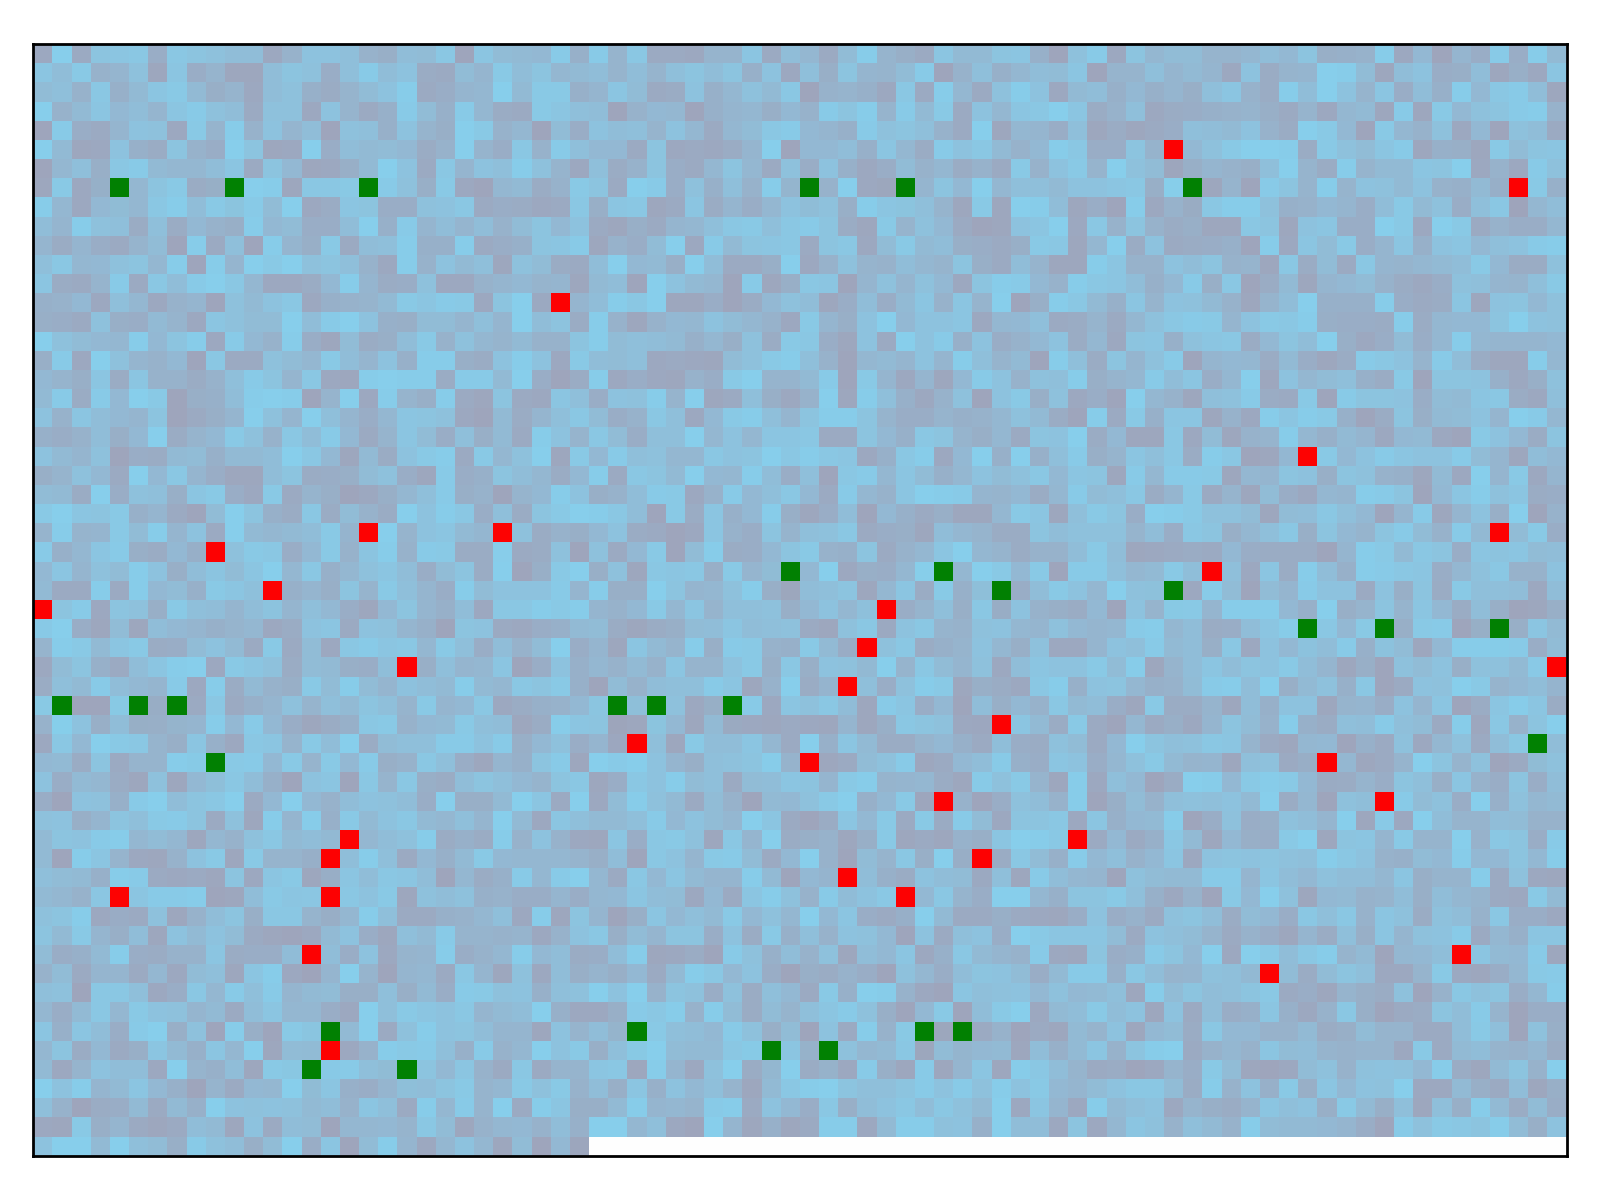
\includegraphics[width=0.75\textwidth]{doc11358_topic0.png} %&
        % 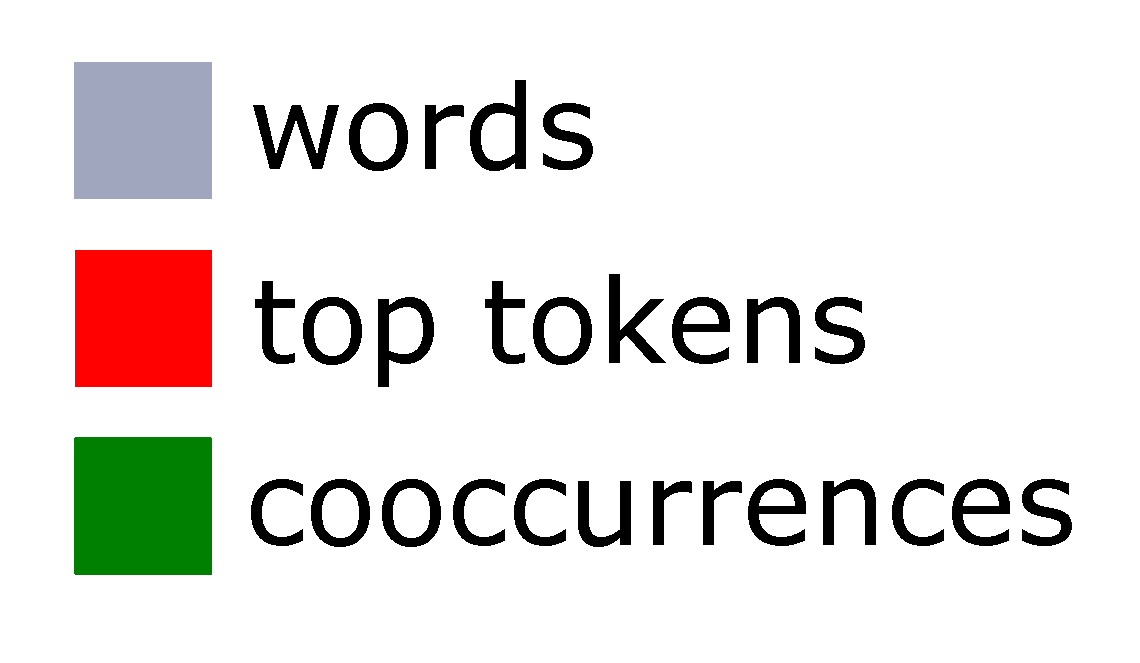
\includegraphics[width=0.25\textwidth]{legend.eps} \\
    %\end{tabular}
    \caption{Демонстрация доли текста, покрытой верхними словами, на примере одного документа. Словопозиции обозначены серо-синим цветом, словопозиции верхних слов показаны красным цветом, зелёным цветом показаны словопозиции, имеющие ненулевой вклад в расчёт когерентности (т.е. попадающие в скользящее окно вместе с другим верхним словом).}
\label{fig:ch3_doc_compound}
\end{figure}


Пусть $Q$ --- некое множество слов. Эти слова встречаются в некоем документе $d$, который можно считать списком словопозиций: $d = [w_1, w_2, w_3, \dots w_{n_1}]$.

Назовём словопозицию $i, ~w_i \in Q$ \textit{представленной}, если существует какое-либо контекстное окно $[w_i, w_{i+1}, w_{i+2}, \dots w_{i+k-1}, w_{i+k}]$, содержащее эту позицию вместе с позицией какого-либо другого слова $v, v \in Q$. Таким образом, словопозиция является \textit{представленной} если и только если у неё ненулевой вклад в счётчики совстречаемости множества $Q$.

Теперь можно сформулировать следующий естественный вопрос: если совстречаемости посчитаны на основе 10 топ-слов одной темы (или сразу нескольких тем), то какая доля словопозиций коллекции \textit{представлена} в этих статистиках?

%  Ясно, что эта величина не может быть больше, чем общая частота топ-слов в коллекции (эта частота обычно лежит в промежутке $1\%$ - $5\%$).

% \dscl{тут стоит расширить эксперименты, посмотреть больше моделей (в том числе и с разной регуляризацией)}

% \dscl{Мне кажется, что тут не хватает двух экспериментов. 1) Представительность нужно посмотреть с другим размером множества топ-токенов (не 10, а 20, 30, 50, 100; отсечение по порогу, а не по константе).}

Мы измерим представительность двух тематических моделей на двух разных коллекциях документов. Первая модель построена на коллекции статей сайта <<ПостНаука>> и состоит из 19 предметных и одной фоновой темы. Вторая модель является наиболее интерпретируемой (согласно экспертам, оценивавшим 10 верхних слов тем) из 9 моделей, рассмотренных в работе~\cite{rtl}. Эта модель построена на подвыборке статей английской <<Википедии>> и состоит из 50 тем.

\begin{table}[ht]
\begin{tabular}{lll}
         & ПостНаука & Википедия \\
Минимум  & 0.0159\%  & 0.0065\%  \\
Медиана  & 0.0483\%  & 0.0293\%  \\
Среднее  & 0.0619\%  & 0.0356\%  \\
Максимум & 0.2764\%  & 0.1149\%  \\
Суммарно & 1.2027\%  & 1.6585\%
\end{tabular}
    \caption{
      Доля коллекции, имеющая ненулевой вклад в счётчики совстречаемости 10 верхних слов. Статистики посчитаны по каждой теме отдельно; строка <<суммарно>> показывает представительность объединённого множества верхних слов всех тем.
    }
    \label{table:represented}
\end{table}

Как можно видеть в таблице \ref{table:represented}, верхние слова покрывают исчезающе малую часть коллекции (менее 2\% корпуса). Когерентность отдельно взятой темы в большинстве случаев учитывает менее тысячной доли всего корпуса текста.

\section{Предлагаемая мера: внутритекстовая когрентность}

Как было замечено ранее, традиционные метрики когерентности неявно основываются на допущении о том, что слова <<хороших>> тем часто встречаются рядом. Это похоже на лингвистическую концепцию \textit{когезии} \cite{halliday1976cohesion}: предложения естественного языка подчинены линейной внутренней структуре. Эта горизонтальная структура организуется
различными синтаксическими и лексическими средствами: союзами, повторами, словами-заместителями, согласованием временных и иных форм \cite{kazachenko2009}.

В данной работе делается предположение, что тексты естественного языка состоят из связных фрагментов, каждый из которых содержит малое число скрытых тем. Из этого следует, что интерпретируемость темы должна оцениваться не как согласованность наиболее частых слов темы, но как согласованность слов темы внутри связных фрагментов текста. Нужно заметить, что частая совместная встречаемость самых вероятных слов тоже косвенно указывает на то, что тема встречается в текстовой коллекции как связный фрагмент текста (см. \ref{sec:corpus_agnostic}).

При помощи этого рассуждения можно построить семейство автоматизированных мер интерпретируемости. Каждая из них будет измерять, насколько <<быстро>> или <<сильно>> меняется тематический профиль соседних слов.

Таким образом, мы меняем порядок вычислений когерентности. Традиционные меры когерентности сначала выделяют какое-то множество слов по их $\phi_{wt}$ и затем анализируют, каким образом эти слова встречаются в тексте. В предлагаемом же методе сначала выделяются все соседние слова текста, распределение $\phi_{wt}$ которых затем анализируется.

Можно предложить несколько принципиально разных подходов к формализации этой идеи.

\begin{figure}
  \small
  \begin{tabularx}{1.0\textwidth}{l| *{3}{Y}|*{3}{Y}|}
    & \multicolumn{3}{c|}{Low variance}
    & \multicolumn{3}{c|}{High variance}\\
    \cline{2-7}
    & русский & поэт & Пушкин & Толстой & Рассел & Эйлер \\
    \begin{tabular}[c]{@{}l@{}}$\begin{smallmatrix}\\ \textcolor{my-red}{Literature} \\\\
    \textcolor{green}{Philosophy} \\\\
    \textcolor{blue}{Mathematics} \\\\
    \end{smallmatrix}$\end{tabular}  &
    \begin{tabular}[c]{@{}l@{}}
      $\smalltopicvector{my-red!50}{green!25}{blue!25}$
    \end{tabular} &
    \begin{tabular}[c]{@{}l@{}}
      $\smalltopicvector{my-red!90}{green!10}{blue!10}$
    \end{tabular} &
    \begin{tabular}[c]{@{}l@{}}
      $\smalltopicvector{my-red!90}{green!10}{blue!10}$
    \end{tabular} &
    \begin{tabular}[c]{@{}l@{}}
      $\smalltopicvector{my-red!90}{green!30}{blue!10}$
    \end{tabular} &
    \begin{tabular}[c]{@{}l@{}}
      $\smalltopicvector{my-red!10}{green!50}{blue!50}$
    \end{tabular} &
    \begin{tabular}[c]{@{}l@{}}
      $\smalltopicvector{my-red!10}{green!10}{blue!90}$
    \end{tabular}
  \end{tabularx}
    \caption{Caption}
    \label{fig:intracohs_pic1}
\end{figure}
\textbf{Средний разброс в окне.} Семантическую близость расположенных рядом слов можно выразить как дисперсию векторов с компонентами $p(t \cond w)$ (см. рис. \ref{fig:intracohs_pic1}). Данная величина подсчитывается в каждом скользящем окне длиной в $p_1$ слов. Другая естественная вариация --- среднее попарное расстояние векторов $p(t \cond w)$ в скользящем окне. Расстояние можно подсчитывать несколькими способами (например, как евклидово расстояние или как косинусную близость).

\begin{figure}
    \noindent
    $\mbox{Группе}\ \underbrace{\mbox{\textcolor{my-pink}{астрономов}}\ \mbox{удалось}}_{l_1=2}\ \mbox{обнаружить}\ \underbrace{\mbox{\textcolor{my-pink}{звезду}}, \mbox{обращающуюся}}_{l_2=2}$\\
    $\mbox{вокруг}\ \underbrace{\mbox{\textcolor{my-red}{чёрной}}\ \mbox{\textcolor{my-red}{дыры}}\ \mbox{на}\ \mbox{рекордно}\ \mbox{близком}}_{l_3=4}\ \mbox{расстоянии}.$
    \caption{Пример. Тема $t = \mbox{<<Чёрные дыры>>}$}
    \label{fig:intracohs_pic3}
\end{figure}

\textbf{Длина сегмента.} Другим показателем тематической однородности может быть средняя продолжительность темы внутри текста. Будем считать, что слово $w$ относится к теме $t$, если разность между компонентой вектора $p(t \cond w)$, отвечающей теме $t$, и максимальной компонентой из оставшихся больше заданного порога (здесь в качестве порога был использован $0$).

На практике оказывается нужен дополнительный механизм, уменьшающий чувствительность меры качества к словам общей лексики. Для этого можно <<разрешить>> ей учитывать чуждые текущей теме слова с небольшим негативным штрафом. Когда величина суммарно набранного штрафа пересекает заданный порог, сегмент отмечается как закончившийся; количество отмеченных слов и будет значением искомой метрики качества (см. рис. \ref{fig:intracohs_pic3}).

\begin{figure}
    \centering
    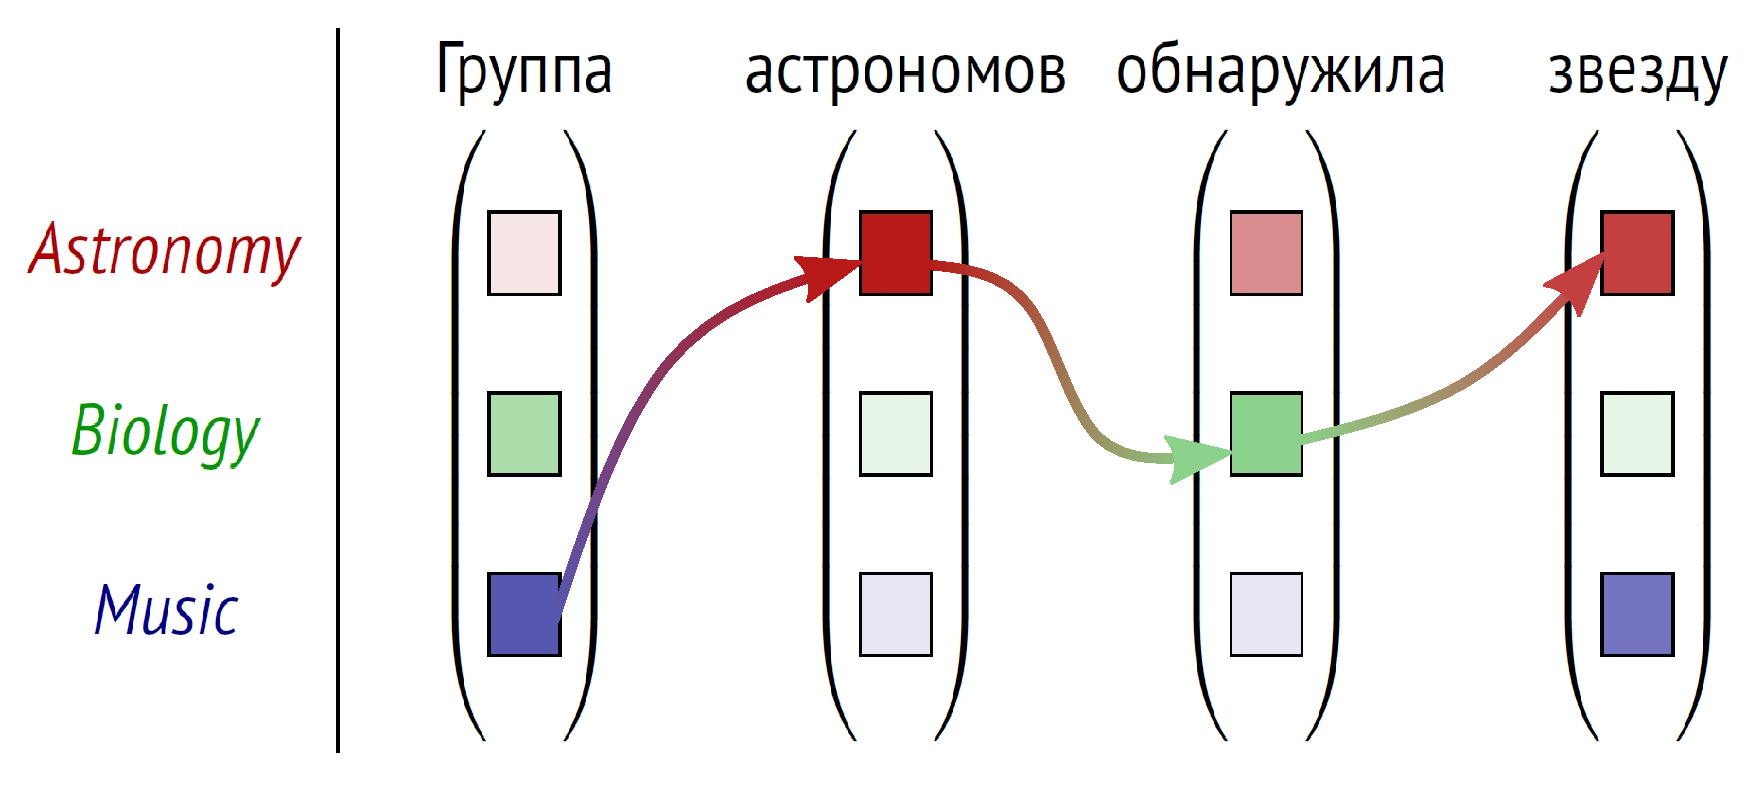
\includegraphics[width=0.8\textwidth, height=0.2\textheight]{astronomers_focon.eps} % .eps image is wrong scaled
    \caption{Caption}
    \label{fig:intracohs_pic2}
\end{figure}

\textbf{Скачки тематики.} Третий подход к измерению внутритекстовой когерентности --- оценивать, как сильно в целом по всему тексту отличаются по тематике смежные слова. Суммируются попарные разности между максимальными вероятностями в каждом векторе $p(t\mid w)$. Подразумевается, что наиболее вероятные темы у соседних слов могут различаться, но тема не должна <<затухать>> слишком быстро (см. рис. \ref{fig:intracohs_pic2}).

Этот подход также требует механизма работы с <<чуждыми>> словами: два слова считаются соседними, если количество принадлежащих фоновой теме слов между ними не больше заданного порога (фоновой считается тема, имеющая больше всего приписанных к ней словопозиций в данном документе).

\section{Постановка задачи}

\begin{figure}[h]
    \centering
    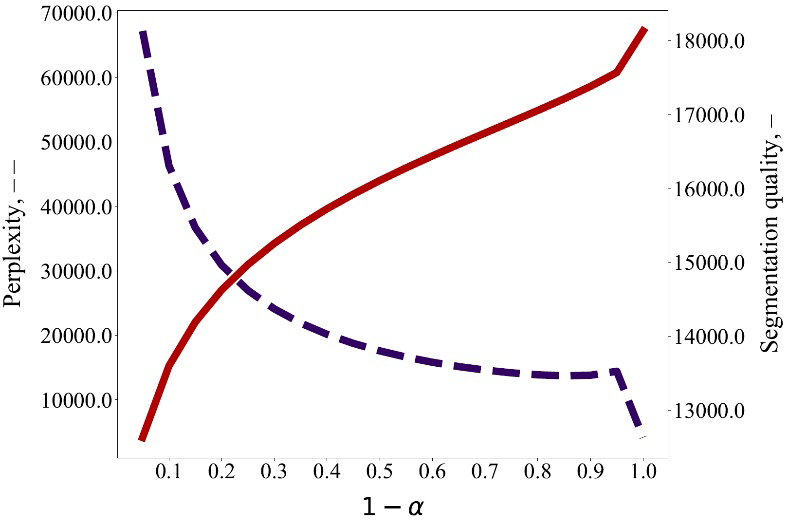
\includegraphics[width=0.8\textwidth]{images/segm_1.png}
    \caption{На графике показана зависимость мер качества от степени деградации матрицы $\Phi$. Согласованность качества сегментации и перплексии говорит о том, что качество сегментации действительно характеризует <<хорошесть>> тематической модели.}
    \label{plot:segm_quality-iteration}
\end{figure}

Оценка интерпретируемости --- очень трудоёмкое мероприятие, даже для процедур, основанных на верхних словах.
В данной работе эта проблема усугубляется. С одной стороны, мы желаем построить меру качества, учитывающую $\Phi$, $\Theta$ и коллекцию документов целиком. С другой стороны, валидация такой метрики требует сравнения её с человеческими оценками интерпретируемости (что означает необходимость разметки огромного массива данных).

Мы предлагаем способ обойтись без этого затруднительного мероприятия: вместо того, чтобы размечать данные вручную, можно сгенерировать полусинтетический корпус с известной разметкой. Структура коллекции <<ПостНаука>> играет в этом важную роль: темы статей настолько обширны и различны, что большинство документов являются \textit{монотематическими}: каждое слово такого документа связано не более чем с одной предметной темой (иными словами, монотематические документы --- это документы, все слова которых являются либо фоновыми, либо относятся к определённой предметной теме). Среди 3446 оригинальных статей исходной коллекции 2118 являются монотематическими.

Полусинтетическая коллекция будет собрана из фрагментов таких монотематических документов. Исходные тексты разбиваются на сегменты, которые перемешиваются и объединяются в новые документы.

% Идея состоит в том, что большие монотематические документы можно разрезать на маленькие монотематические сегменты, которые затем будут случайно сшиты вместе.

В результате этого процесса получается коллекция данных с известным общим числом тем, распределением тем в документах и даже известными метками тем для слов. Отметим, что любая тематическая модель неявно классифицирует слова заданного документа по темам. Действительно, любому слову $w$ из документа $d$ соответствует величина $p_{tdw} = p(t \cond d, w) \propto \phi_{wt}\theta_{td}$, задаваемая тематической моделью. Таким образом, полусинтетическая коллекция позволяет определить эталонную меру качества произвольной тематической модели, измеряя соответствие между $p_{tdw}$ и <<эталонной>> меткой слова $w$. Назовём эту меру \textit{качеством сегментации} данной тематической модели.

Качество сегментации текста тематической моделью оценивается <<мягким>> образом: для каждой темы $t$ считается сумма $p(t \mid d, w)$ на всех парах $(d,~w),\ d~\in~D, w~\in~W_d$, итоговый результат~---~сумма таких сумм по всем темам. Для того чтобы вычислить указанные выше величины, необходимо знать соответствие между темами, выданными моделью, и темами исходного датасета статей <<ПостНауки>>. Для этого использовался венгерский алгоритм \cite{kuhn1955hungarian}, выдающий наиболее удачное соответствие тем модельная-исходная.

Искомый процесс оценки различных мер качества будет построен следующим образом. Пусть дано множество различных тематических моделей. Для каждой модели можно вычислить её качество сегментации и различные рассматриваемые меры качества (как традиционные меры когерентности, так и предлагаемые меры внутритекстовой когерентности). Таким образом, каждой модели $m_i$ можно сопоставить набор численных значений $f_j(m_i)$ --- замеры её качества при помощи различных методов $f_j$. Величина, которая будет показывать качество какого-либо из методов --- коэффицент корреляции Спирмана между $f_j(m_i)$ и качеством сегментации $m_i$ по всем возможным $m_i$.

Рассматриваются шесть мер качества: 
\begin{itemize}
    \item \texttt{Newman} (также называемый UCI-когерентностью) вычисляется как средний попарный PMI среди всех верхних токенов. Статистика совстречаемостей вычисляется на данном полусинтетическом датасете.
    \item \texttt{Mimno} (также называемый UMass-когерентностью) вычисляется как средний логарифм отношения $p(w_i, w_j)$ к $p(w_j)$, взятый по всем парам слов $(w_i,~w_j)$, в которых $w_j$ более вероятно в теме $t$, нежели слово $w_i$ (т.е. условной вероятности менее вероятного слова с учётом более вероятного). Статистика совстречаемостей вычисляется на данном полусинтетическом датасете. 
    \item  \texttt{SemantiC\_L2}~---~предлагаемый критерий качества, основанный на попарном евклидовом расстоянии между тематическими векторами.
    \item  \texttt{SemantiC\_Var}~---~предлагаемый критерий качества, основанный на дисперсии тематических векторов в окне.
    \item  \texttt{TopLen}~---~предлагаемый критерий качества, основанный на средней длине тематических сегментов в тексте.
    \item  \texttt{FoCon}~---~предлагаемый критерий качества, учитывающий скачки тематик соседних слов.
\end{itemize}

В данной работе мы ставим задачу показать, что в серии моделей с улучшающейся интерпретируемостью внутритекстовые меры когерентности монотонно возрастают, в то время как способы оценки когерентности по верхним словам этого не делают.

\section{Вычислительный эксперимент}

\begin{figure}[h]

    \centering
    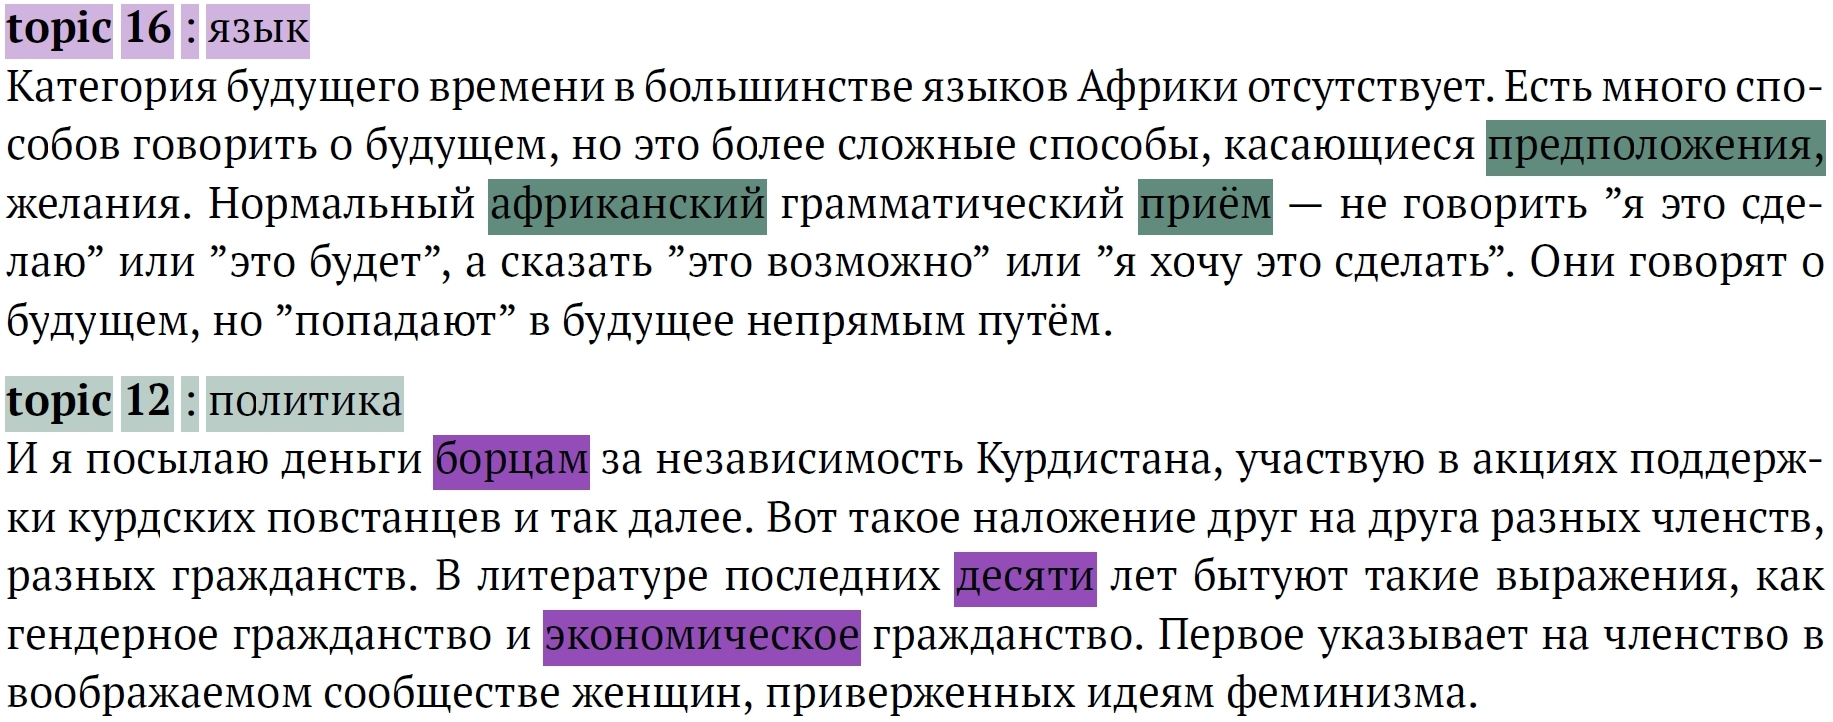
\includegraphics[width=\textwidth]{combine_bad.jpg}

  %\vspace{-0.5cm}
    \scriptsize
    \centering
    \begin{tabular}{rrrrrrrr}
      Сегментация & UCI & UMass & SemantiC L2 & SemantiC Var & TopLen & FoCon\\
      \midrule
      \rowcolor{my-blue-light}
      11000 & -4.8 & -3.1 & -13 & -37000 & 2.9 & -140000\\
      \textbf{38000} & \textbf{-3.7} & \textbf{-2.7} & \textbf{-3.7} & \textbf{-8100} & \textbf{3.5} & \textbf{-54000}
    \end{tabular}
  %\vspace{-0.5cm}

    \centering
    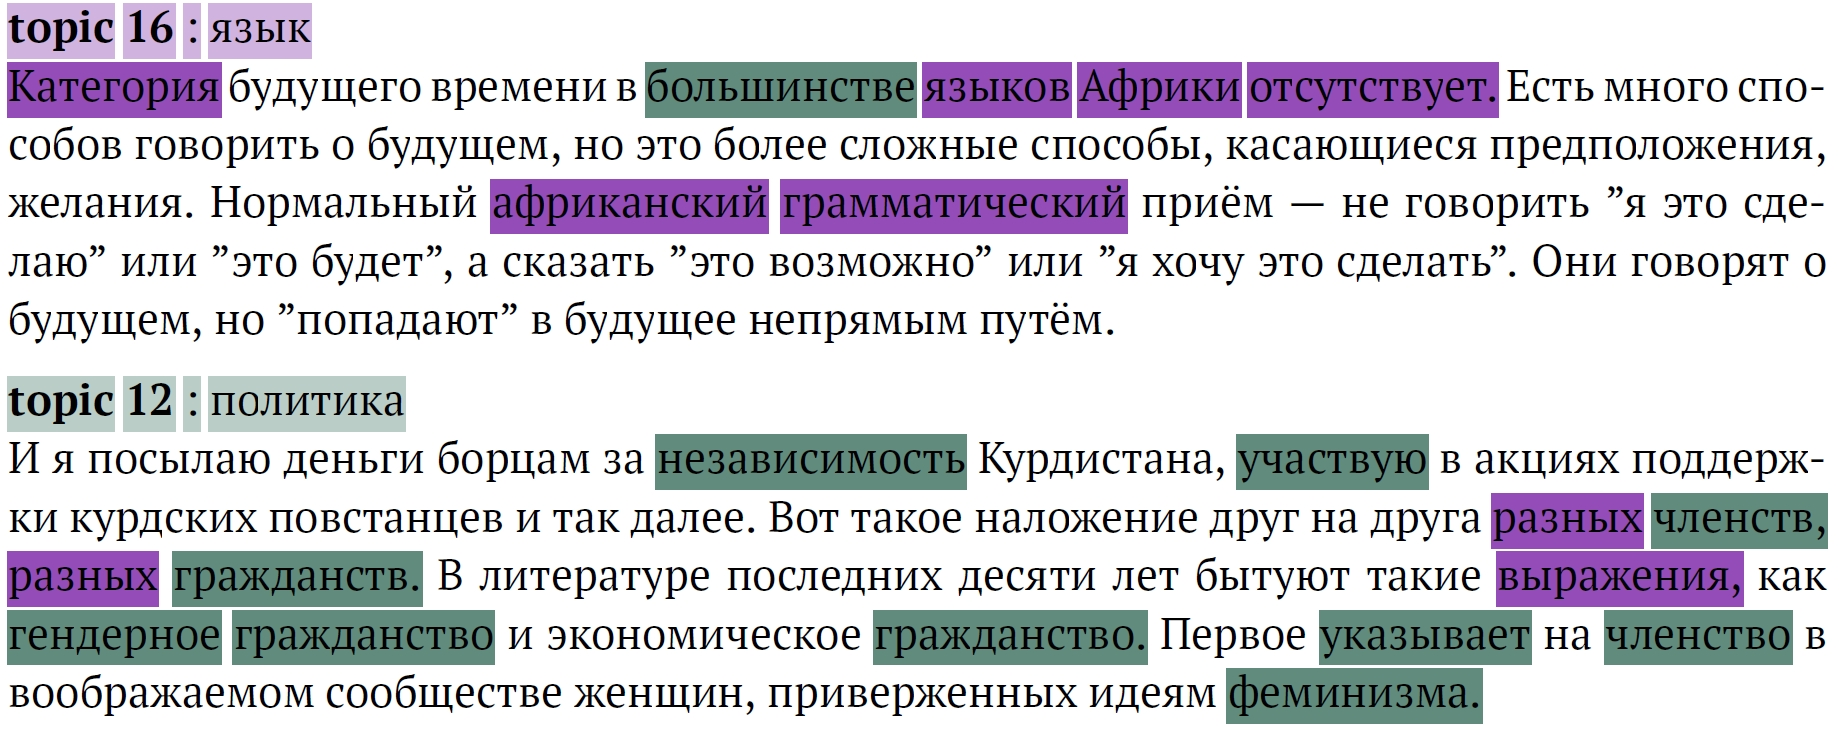
\includegraphics[width=\textwidth]{combine_good.jpg}

    \scriptsize
    \centering
    \begin{tabular}{rrrrrrrr}
      Сегментация & UCI & UMass & SemantiC L2 & SemantiC Var & TopLen & FoCon\\
      \midrule
      11000 & -4.8 & -3.1 & -13 & -37000 & 2.9 & -140000\\
      \rowcolor{my-blue-light}
      \textbf{38000} & \textbf{-3.7} & \textbf{-2.7} & \textbf{-3.7} & \textbf{-8100} & \textbf{3.5} & \textbf{-54000}
    \end{tabular}
  %\vspace{-0.5cm}

    \caption{Рисунок показывает фрагмент одного из сгенерированных документов, который состоит из двух соседних сегментов различных тем длиной 50 слов. Слова сегментов обработаны описанными ранее <<хорошей>> моделью и <<плохой>> моделью. Нераскрашенные слова были отнесены к какой-либо теме, отличной от двух <<главных>>. Также приведены численные величины различных когерентностей и значения, характеризующие качество сегментации. Полужирным отмечены ситуации, в которых значение когерентности возрастает при улучшении качества модели.}
    \label{fig:segm_good_bad}
\end{figure}




График \ref{plot:segm_quality-iteration} показывает, как ведёт себя качество мягкой сегментации при увеличении внутренней меры качества тематической модели.

Выборка тематических моделей, по которой рассчитывалась корреляция Спирмана, представлет собой параметризованное параметром $\alpha$ семейство. Матрица $\Phi$ модели из этого семейства является взвешенной комбинацией

\[
m(\alpha) = \alpha \Phi_{bad} + (1-\alpha)\Phi_{good},
\]

где $\Phi_{good}$ --- матрица $\Phi$ описанной выше модели корпуса <<ПостНауки>>, а $\Phi_{bad}$ --- набор случайных столбцов, порождённых распределением Дирихле ($0.01^{|W|}$). Были проведены четыре серии экспериментов с различными матрицами $\Phi_{bad}$. На рисунке \ref{fig:segm_good_bad} показано различие качества этих моделей на примере сегментации одного из документов.

\subsection{Результаты}
Представлены три метода оценки интерпретируемости тематических моделей: SemantiC, TopLen и FoCon. В отличие от традиционных оценок когерентности, предложенные методы пытаются учесть все словопозиции коллекции.

Для того чтобы сравнить предложенные меры качества с двумя традиционными метриками (Newman и Mimno), был проведён эксперимент на полусинтетическом датасете, составленном из сегментов различных тем.

В экспериментах анализировались корреляции между значениями когерентностей и качеством сегментации текстов. Два из предложенных методов --- SemantiC и TopLen --- и существующая метрика UMass-когерентность показывают высокие корреляции с качеством сегментации.

\begin{figure}
\begin{tabular}{cc}
    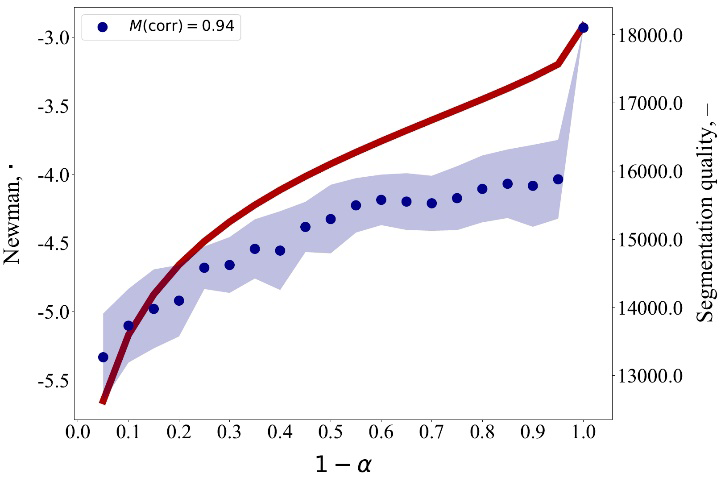
\includegraphics[width=70mm]{images/segm_mimno.png} &   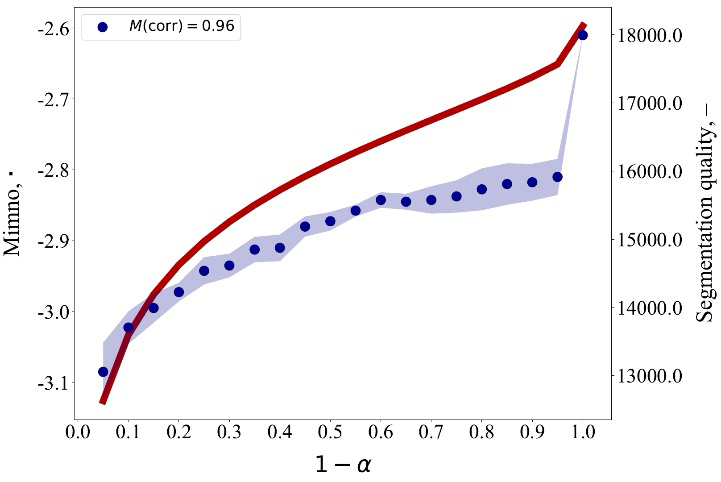
\includegraphics[width=70mm]{images/segm_newman.png} \\
 
    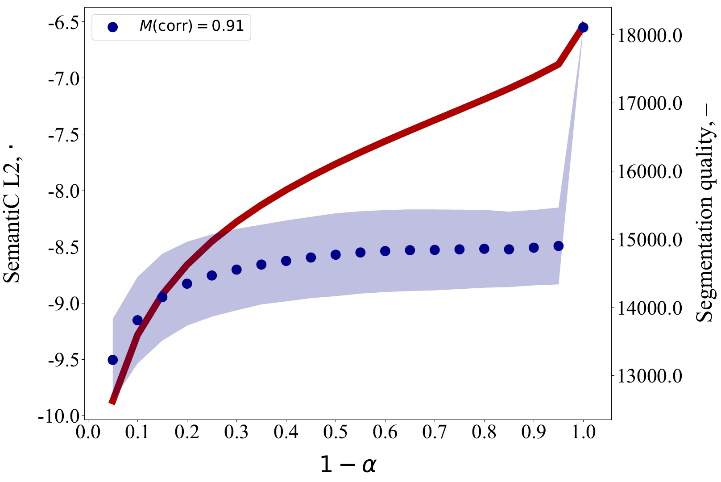
\includegraphics[width=70mm]{images/segm_l2.png} &   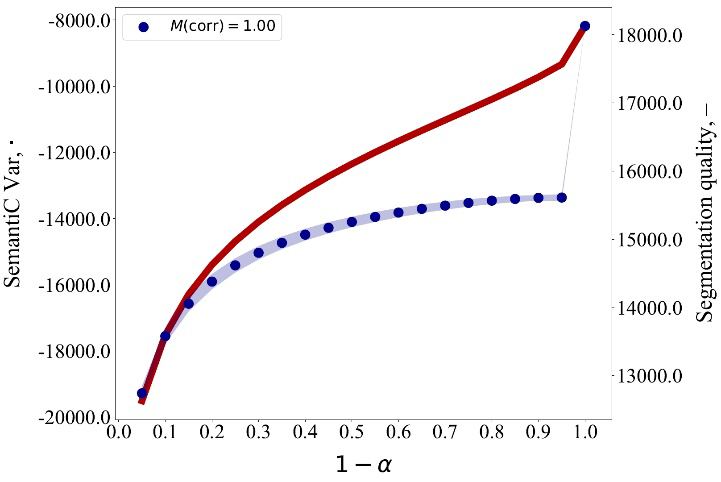
\includegraphics[width=70mm]{images/segm_var.png} \\
 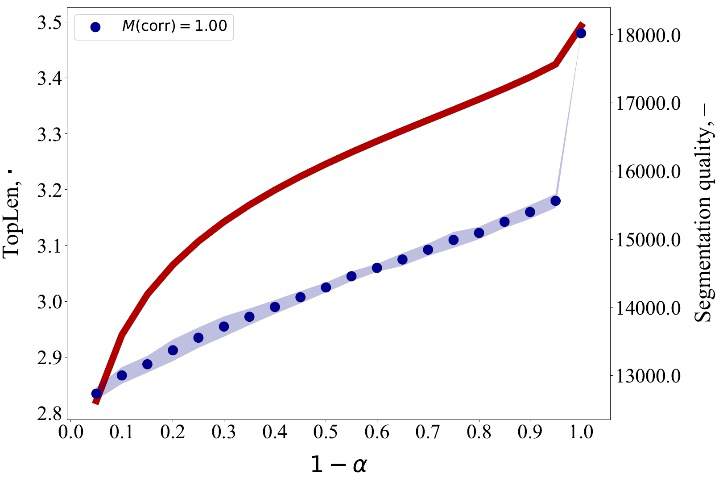
\includegraphics[width=70mm]{images/segm_toplen.png} &   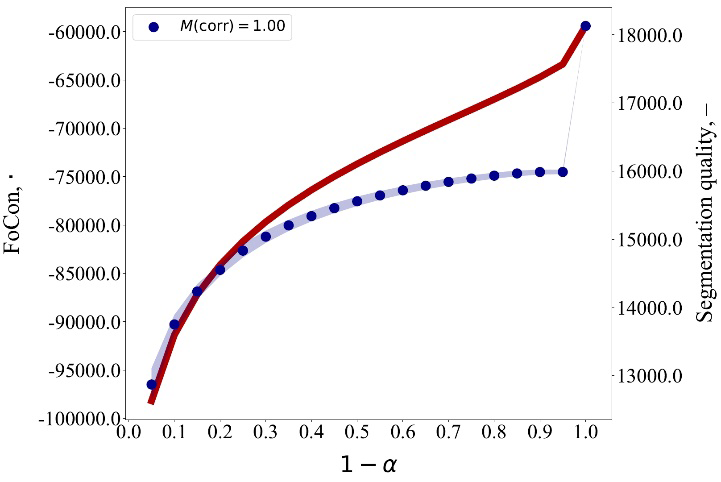
\includegraphics[width=70mm]{images/segm_focon.png} \\
\end{tabular}
    \caption{Сравнение различных мер когерентности и качества сегментации, нарисованное как функция от степени деградации тематической модели $\alpha$. }
\label{fig:ch3_corr}
\end{figure}




% SQ (S) --- мягкая segmentation quality, SQ (H)—strict segmentation quality, N—Newman, M—Mimno, SC—SemantiC, TL—TopLen, FC—FoCon.
 
           % Глава 3
\chapter{Повышение интерпретируемости тематических моделей при помощи регуляризации}

В этом разделе будет предложен метод подбора коэффициентов сглаживания, коэффициентов разреживания и весов дополнительных модальностей. Также будет рассмотрен псевдорегуляризатор, основанный на допущении о функциональной зависимости $\Theta = f(\Phi)$ и превносящий в тематическую модель много полезных свойств.

В данной главе ставится цель проанализировать поведение предложенного алгоритма на реальных текстовых коллекциях.

\section{Относительные коэффициенты регуляризации}

% Задача этого текста --- обьяснить теоретическую подоплёку относительных коэффициентов регуляризации и дать ряд практических советов по их применению.

% В данный момент открытая библиотека bigARTM умеет работать с относительными коэффициентами для $\phi$-регуляризаторов. Таким же образом можно подбирать и коэффициенты для $\theta$-регуляризаторов (возможность, которая сейчас в bigARTM отсутствует). Более того, таким же образом можно и подбирать веса дополнительных модальностей (возможность, которая и не снилась нашим мудрецам).

Относительные коэффициенты регуляризации были впервые введены в работе \cite{doykov} в общем виде.

\dscl{Общая формула взята из ВКР Никиты Дойкова. Важные частные случаи --- выведены мной, успешно проверены на практике}
В исследовании \cite{doykov} приведена формула для общего случая $k$ произвольных гладких регуляризаторов $R_i(\Phi, \Theta)$. Здесь и далее: $\tau_i$ (тау) обозначает абсолютный коэффициент регуляризации, а $\lambda_i$ - относительный коэффициент регуляризации

Общая формула для регуляризаторов $\Phi$:
\[
\phi_{wt} = \norm_{w \in W}\Bigg( 
    n_{wt} + \sum_{i=1}^k \lambda_i \Big[
        \gamma_i \frac{n_t}{r_{it}} + (1-\gamma_i)\frac{n}{r_i}
        \Big] 
    \phi_{wt} \frac{\partial R_i}{\partial \phi_{wt}}
\Bigg), \label{rel_phi_general}
\]

где: 
\begin{itemize}
    \item{$r_{it} = \sum_{w\in W} \Big| \phi_{wt} \frac{\partial R_i}{\partial \phi_{wt}} \Big| $ --- воздействие регуляризатора на тему}
    \item { $r_{i} = \sum_{t\in T} r_{it}$ --- суммарное воздействие регуляризатора на коллекцию.}
    \item { $\lambda_i$ - относительный коэффициент регуляризации, показывающий, \emph{во сколько раз} соответствующий регуляризатор влияет на оценку $\phi_{wt}$ больше, чем коллекция}
    \item {Выражение в квадратных скобках - \textit{фактор балансировки}, гарантирующий ''равновесие'' между $n_{wt}$ и регуляризационной добавкой}
\end{itemize}

Введённый в этой формуле коэффициент $\gamma_i$ отвечает за степень индивидуализации. Он позволяет плавно переходить от равномерной регуляризации по всем темам ($\gamma = 0$) к индивидуальному подходу к каждой теме ($\gamma = 1$).

Важно заметить следующие особенности: 
\begin{enumerate}
    \item {В формуле участвуют $n_t, r_{it}, r_{i}$:  величины, которые могут изменяться в ходе итераций EM-алгоритма. Следовательно, в общем случае
    абсолютные коэффициенты и относительные  коэффициенты задают различные множества возможных траекторий регуляризации.}
    \item  {В формуле участвуют $n_t, r_{it}, r_{i}$: переменные, значения которых определяются в ходе ЕМ-алгоритма.}
\end{enumerate}

Общая формула для регуляризаторов $\Theta$:

\[
\theta_{td} = \norm_{t \in T} \Bigg( 
    n_{td} + \sum_{i=1}^k \lambda_i \Big[
        \gamma_i \frac{n_d}{r_{id}} + (1-\gamma_i)\frac{n}{r_i}
        \Big] 
    \theta_{td} \frac{\partial R_i}{\partial \theta_{td}}
\Bigg), \label{rel_theta_general}
\]

где: 
\begin{itemize}
    \item { $r_{id} = \sum_{t\in T} \Big | \theta_{td} \frac{\partial R_i}{\partial \theta_{td}} \Big | $ --- воздействие регуляризатора на документ}
    \item { $r_{i} = \sum_{d\in D} r_{id}$ --- суммарное воздействие регуляризатора на коллекцию.}
    \item { $\lambda_i$ - относительный коэффициент регуляризации, показывающий, \emph{во сколько раз} соответствующий регуляризатор влияет на оценку $\theta_{td}$ больше, чем коллекция}
    \item {Выражение в квадратных скобках - \textit{фактор балансировки}, гарантирующий ''равновесие'' между $n_{td}$ и регуляризационной добавкой}
\end{itemize}

Вычисления по формуле \ref{rel_theta_general} являются проблематичными для онлайнового и пакетных ЕМ-алгоритмов. Это связано с тем, что алгоритм разбивает коллекцию документов на пакеты, обрабатываемые параллельно и связанные только посредством матрицы $\Phi$. Поскольку в общем случае вычисление $r_i$ требует информацию о всех документах сразу, то формула \ref{rel_theta_general} несовместима с архитектурой эффективного ЕМ-алгоритма.

Тем не менее, для ряда важных частных случаев подобрать относительные коэффициенты регуляризации всё-таки возможно.

\subsection{Важные частные случаи}
\dscl{Здесь есть неотвеченный вопрос: как в БигАРТМ работает относительная декорреляция. Фактор балансировки там скачет от итерации к итерации, мне кажется что этот вопрос стоит доисследовать}

\textbf{Утверждение}. Для регуляризаторов сглаживания и разреживания, каждый абсолютный коэффициент регуляризации математически равносилен некоторому относительному коэффиценту и наоборот.

\textbf{Сглаживание и разреживание Фи}. Формула M-шага, сглаживающего ($\tau > 0$) или разреживающего ($\tau < 0$) распределение $\phi_{wt}$:

\[
\phi_{wt} = \norm_{w \in W} \big( n_{wt} + \tau \big)
\]

Интуитивный смысл этого преобразования прост: мы либо ''притягиваем'' Фи к равномерному распределению $\beta = \frac{1}{|W|}$, либо ''отталкиваем'' её от него же (возможно, даже зануляя при этом какие-то компоненты).

Оказывается, можно провести репараметризацию, которая строго это продемонстрирует. 

Пусть $\beta = \frac{1}{|W|}$ --- равномерное распределение, а текущие значения $n_{wt}$ и $\tau \in \mathbb{R}$ таковы, что на этой итерации M-шага зануления компонент не происходит (то есть либо $\tau > 0$, либо $\tau < 0$, но $n_{wt} + \tau > 0$).

Тогда операцию положительной обрезки можно проигнорировать:

\[
\phi_{wt} = \norm_{w \in W} \big( n_{wt} + \tau \big) = \frac{n_{wt} + \tau }{\sum_{w \in W} n_{wt} + \tau } = \frac{n_{wt} + \tau }{n_{t} + \tau |W|}  
\]

Попробуем представить это выражение, как выпуклую комбинацию распределений  $\frac{n_{wt}}{n_t}$ (оценки максимума правдоподобия) и $\frac{1}{|W|}$ (равномерного распределения). 


\[
\frac{n_{wt} + \tau}{n_{t} + \tau |W|} = (1-\lambda) \frac{n_{wt}}{n_t} + \lambda \frac{1}{|W|} \iff \tau  = \frac{n_t \lambda}{(1-\lambda) |W|} \label{sp_phi_rel2abs} 
\]

Значит, сглаживание Фи можно трактовать, как нахождение компромисса между $\phi_{wt} = \frac{n_{wt}}{n_t}$ и $\phi_{wt} = \frac{1}{|W|}$. 

Что это означает на практике? Допустим, мы хотим провести регуляризацию так, чтобы $\phi_{wt}$ на 50\% состояла из оценки максимума правдоподобия, и на 50\% из априорного распределения $\frac{1}{|W|}$. Для этого достаточно вычислить $\tau$ по формуле и подставить в модель.

Важно заметить следующие особенности: 

\begin{enumerate}
    \item  {Полученный коэффициент регуляризации зависит от $n_t$, то есть разные темы будут сглаживаться/разреживаться с разной силой}
    \item  {Поскольку значение $n_t$ может изменяться в ходе итераций EM-алгоритма, то абсолютная величина коэффициента тоже может меняется со временем}
    \item  {Зависит от $|W|$. Это значит, что один и тот же абсолютный коэффициент сглаживания/разреживания может по-разному влиять на коллекцию в зависимости от размера словаря.  Формула \ref{sp_phi_rel2abs} делает эту зависимость более наглядной. Теперь можно эвристически прикинуть, как нужно пересчитать $\tau$ при изменении словаря (например, после выкидывания слишком редких или частых слов).}
\end{enumerate}

Особенность (1) добавляет гибкости, но может быть проблематична на практике (слишком много дополнительных степеней свободы, возможен оверфиттинг).

В работе \cite{doykov} было предложено усреднить по всем темам:

\[
\tau = \frac{1}{|T|} \sum_t \tau_t = \frac{n}{|T|\cdot|W|} \frac{\lambda}{(1-\lambda)}
\]

\textbf{Сглаживание и разреживание Теты}. Вспомним, что M-шаг для Теты выглядит таким образом:

\[
\theta_{td} = \norm_{t \in T} \big( n_{td} + \tau \big)
\]

Аналогично выведем формулу:

\[
\frac{n_{td} + \tau}{n_d + \tau |T|} = (1-\lambda) \frac{n_{td}}{n_d} + \lambda \frac{1}{|T|} \iff \tau = \frac{n_d \lambda}{(1-\lambda) |T|} \label{sp_theta_rel2abs} 
\]

Полученный коэффициент регуляризации зависит от $n_d$, то есть разные документы будут сглаживаться/разреживаться с разной силой. Можно также усреднить все $\tau$ по документам:

\[
\tau = \frac{\lambda \sum_d n_d }{(1-\lambda) |D| \cdot |T|} 
\]

Заметим, что обе формулы для $\tau$ \textit{стабильны}. В отличии от $n_t$, значение $n_d$ в ходе обучения \emph{не меняется}. Все использованные здесь величины заранее известны и постоянны.

Следовательно, если рассматривать лишь усреднённые коэффиценты, то каждый относительный коэффициент регуляризации математически равносилен некоторому абсолютному коэффиценту и наоборот.

\textbf{Многомодальное тематическое моделирование}


Вспомним, что вероятность появления термина $w$ из $k$-й модальности в документе $d$ задаётся следующей формулой:
$p(w^k \cond d) = \sum_t \phi_{wt}^k \theta_{td}$, а общее правдоподобие представляется так:

\[
L(\Phi^m, \Theta) = \sum_m \tau_m \sum_{d\in D} \sum_{w \in W^m} n_{dw} \ln p(w \cond d) \rightarrow \max, \label{modal_likelihood}
\]
где коэффиценты $\tau_m$ показывают \textit{вес} модальности $m$.

Известно, что $EM$-алгоритм для мультимодальной тематической модели структурно похож на классический $EM$-алгоритм \cite{yanina}\cite{vorontsov2015non}\cite{bulatov}. 

Формулу \ref{modal_likelihood} можно проинтерпретировать, как введение $M-1$ дополнительного регуляризатора с коэффициентами $\tau_m$ \cite{yanina}:

\[
\tau_m R(\Phi, \Theta)_m = \tau_m L^{(m)}(\Phi, \Theta) = \tau_m  \sum_d \sum_w n_{dw}^{(m)} \ln \sum_t \phi_{wt}^{(m)}\theta_{td} = 
\sum_d \sum_w \check{n}_{dw}^{(m)} \ln \sum_t \phi_{wt}^{(m)}\theta_{td},
\]

где для удобства было введено ''обобщённое число слов'' $\check{n}_{dw}^{(m)} = \tau_m n_{dw}$ и аналогичные величины $\check{n}_{dt}^{(m)} = \sum_w \check{n}_{dt}^{(m)} p_{tdw}, \check{n}_t = \sum_d \check{n}_{dt}$.

Несложно показать, что выражение $r_{md}$ для этого случая выглядит следующим образом:

\[
r_{md} = \sum_t |\theta_{td} \frac{\partial R_m}{\partial \theta_{td}}| = \sum_t \sum_w \check{n}_{dw}^{(m)} p_{tdw} = \sum_t  \check{n}_{dt}^{(m)} = \check{n}_{d}^{(m)}
\]

Иными словами, $r_{md}$ равняется просто числу токенов модальности $m$ в документе $d$ (с учётом коэффициента $\tau_m$), а $r_m$ равняется просто суммарному количеству токенов этой модальности во всей коллекции (также с учётом коэффициента $\tau_m$).

Без ограничения общности примем, что в модели нет других регуляризаторов и задана лишь одна дополнительная модальность. Подставим найденные значения в формулу \ref{rel_theta_general}:

\[
\theta_{td} = \norm_{t \in T} \Bigg( 
    n_{td} + \lambda_m \Big[
        \gamma_m \frac{n_d}{r_{md}} + (1-\gamma_m)\frac{n}{r_m}
        \Big] 
    \theta_{td} \frac{\partial R_m}{\partial \theta_{td}}
\Bigg) = 
\]
\[
\norm_{t \in T} \Bigg( 
    n_{td} + \lambda_m \Big[
        \gamma_m \frac{n_d}{\check{n}_d^{(m)}} + (1-\gamma_m)\frac{n}{\sum_d \check{n}_d^{(m)}}
        \Big] 
    \theta_{td} \frac{\partial R_m}{\partial \theta_{td}}
\Bigg)
\]

Иными словами, фактор балансировки, ''уравновешивающий'' влияние слов и дополнительной модальности $m$, задаётся через отношение числа токенов модальности $m$ к числу слов в документе (либо во всей коллекции).

Заметим, что фактор балансировки выражается через константы, известные ещё на этапе построения коллекции.

Более того, если рассматривать лишь усреднённые коэффиценты, то каждый относительный вес модальности математически равносилен некоторому абсолютному весу и наоборот.

\[
\tau_m = \lambda_m \frac{n}{\sum_d \check{n}_d^{(m)}} \iff 
\lambda_m = \tau_m \frac{\sum_d \check{n}_d^{(m)}}{n}
\]


\subsection{Использование на практике}

Как я уже показал выше, можно адаптивно сглаживать/разреживать тету. Ещё один метод, полезный на практике, связан с весами модальносстей.

Формулы, задающие перевод из одного в другое, не требуют сложных выкладок. Их можно вычислить не только в ядре bigARTM, но даже внутри внешнего python-интерфейса.

В отличии от абсолютных коэффицентов/весов, 
относительные коэффициенты/веса можно интерпретировать, что упрощает процесс настройки тематической модели.

Можно уверенно утверждать, что относительные коэффициенты/веса являются мощным инструментом для тематического моделирования в рамках bigARTM и заслуживают повсеместного использования. 

Абсолютные и относительные коэффициенты сглаживания/разреживания для $\Theta$ эквивалентны. То же самое можно утверждать про абсолютные и относительные веса модальностей. 

\section{Аддитивная регуляризация тематических моделей c
быстрой векторизацией текста}

\section{Мотивация}

\subsection{Важность матрицы тем в документах}
С точки зрения вероятностного вывода матрица слова-темы $(\Phi)$ и матрица документы-темы $(\Theta)$ имеют одинаковую важность, поскольку обе являются скрытыми параметрами вероятностной модели. Однако, на практике, исследователи часто считают матрицу $\Phi$ более важной и относятся к матрице $\Theta$ как к чему-то вспомогательному, что может быть легко восстановлено из известных данных.

В первую очередь нужно упомянуть интерпретируемость. Интерпретируемость является желательным свойством хорошей тематической модели. Оценка интерпретируемости человеком обычно состоит из выбора небольшого набора самых вероятных слов для каждой темы и представления этого набора эксперту-человеку \cite{roder2015exploring}. В этом процессе используется только матрица $\Phi$.

Вторым примером подобного подхода является основополагающая работа \cite{rtl}, в которой измерялась интерпретируемость нескольких тематических моделей. Построенные модели вместе с использованной разметкой, были выложены в открытый доступ. Однако, была опубликована только матрица $\Phi $ (возможно, потому что авторы посчитали ее более ценной, или из-за неявного расчёта на то, что недостающее распределение $\Theta$ может быть восстановлено по выложенным данным).

К второстепенности матрицы $\Theta$ можно прийти и из практических соображений.

Во-первых, на практике часто встречаются задачи, требующие динамического расширения коллекции документов (например, анализ новостных потоков). Такое расширение может существенно увеличить $\mid D\mid$, практически не изменив размер словаря $\mid W \mid$ (что объясняется законом Ципфа \todo{cite something else, not powers-1998-applications}).

Во-вторых, требование вычислительной эффективности естественным образом приводит к использованию параллельных, распределённых или онлайновых реализаций алгоритмов тематического моделирования. Наиболее эффективным является следующий подход, реализованный в открытой библиотеке BigARTM: алгоритм разбивает входные данные на пакеты, которые обрабатываются разными потоками \cite{frei2016parallel}. В результате, алгоритмы библиотеки никогда не хранят всю матрицу $\Theta$, вместо этого элементы матрицы рассчитываются, когда они необходимы.

Сложившуюся ситуацию можно назвать парадоксальной. Для многих исследователей качество тематической модели эквивалентно прежде всего качеству матрицы $\Phi$. Но с точки зрения самой тематической модели, $\Phi$ и $\Theta$ являются равноправными, и появление слов в документах коллекции объясняется при помощи обеих этих матриц. Качество матрицы $\Theta$ при этом никак не контролируется, поэтому тематическая модель может скомпенсировать ``плохую'' $\Phi$ специально подогнанной матрицей $\Theta$.

\subsection{Матрица тем в документах и EM-алгоритм}
\label{sec:theta_inference}

Реализации тематического моделирования (особенно  восстанавливающие элементы $\Theta$ ``на лету'') часто используют следующую эвристику: для получения $\theta_{td}$ конкретного документа $d$ повторяются несколько итераций EM-алгоритма с фиксированной $\Phi$. В этой процедуре вектор $\theta_{\ast d}$ сначала инициализируется некоторым образом (как правило, используется равномерное распределение), а затем итеративно обновляется по формуле $\theta_{td}  \propto \sum_{w} n_{dw} p_{tdw}$ с пересчётом $p_{tdw}$. Обновление может происходить какое-то установленное количество итераций либо продолжаться до сходимости.

Отметим, что этот процесс может привести к переобучению, поскольку $\Theta$ целенаправленно оптимизируется для того, чтобы соответствовать заданной $\Phi$. Кроме того, время обучения модели линейно зависит от числа этих итераций, и поэтому слишком большое их количество может существенно замедлить обучение.

Чтобы формализовать этот происходящий на практике подход, мы предлагаем заменить исходную оптимизационную задачу \ref{eq:EM} на следующую:
\begin{equation} \label{eq:tEM}
L(\Phi, f(\Phi) ) + R(\Phi, f(\Phi) ) \to \max_{\Phi},
\end{equation}

где $f$ --- это некоторая функция, которая отображает матрицу темы-слова в матрицу документы-темы. Решение задачи \ref{eq:tEM} может отличаться от решения задачи \ref{eq:EM}.

Естественный кандидат для функции зависимости $\Phi$ и $\Theta$ --- одна итерация процесса, описанного в \ref{sec:theta_inference} с равномерным начальным приближением $\theta^0_{td} = \frac1{|T|}$. 

\begin{equation}
\label{eq:thetaform}
    \theta_{td}(\Phi)
    = \norm_{t\in T} \biggl( \sum_{w\in W} n_{dw} p_{tdw} \biggr)
    = \sum_{w\in d} \frac{n_{dw}}{n_d} \frac{\phi_{wt} \theta^0_{td}}{\sum_s \phi_{ws} \theta^0_{sd}}
    = \sum_{w\in d} p_{wd} \frac{\phi_{wt}}{\sum_s \phi_{ws}},
\end{equation}
где $p_{wd} = \frac{n_{dw}}{n_d} = \hat p(w\cond d)$~---
частотная оценка условной вероятности терма в~документе. Формулу можно проинтерпретировать как усреднение $n_{dw} P(t \mid w)$) по всем $w \in d$.

\subsection{EM-алгоритм с быстрой векторизацией документов}
\begin{Theorem}
\label{th:TARTM}
    Пусть функция $R(\Phi,\Theta)$ непрерывно дифференцируема, а $\Theta$ находится в функциональной зависимости от $\Phi$ согласно формуле \ref{eq:thetaform}.
    Тогда точка $\Phi$ локального экстремума задачи
    \eqref{eq:tEM} с~ограничениями \eqref{eq:logL.constraints}
    удовлетворяет системе уравнений со вспомогательными переменными, перечисленными ниже:

\begin{align*}
    h_w         &= \bigl( \textstyle\sum_t \phi_{wt} \bigr)^{-1}; \\
    \theta_{td} &= \sum_{w\in d} p_{wd} \phi_{wt} h_w; \\
    p_{tdw}     &= \norm_{t\in T} \bigl(\phi_{wt}\theta_{td} \bigr); \\
    c_{td}      &= \frac1{\theta_{td}}\sum_{w\in d} n_{dw}p_{tdw} + \frac{\partial R}{\partial \theta_{td}}; \\
    \gamma_{dw} &= \sum_{t\in T} \phi_{wt} c_{td}; \\
    p'_{tdw}    &= p_{tdw} + n_d^{-1} \phi_{wt}h_w (c_{td}-h_w\gamma_{dw});
\\
    \phi_{wt} &= \norm_{w\in W}
        \biggl(\,
        \sum_{d\in D} n_{dw} p'_{tdw}
        + \phi_{wt} \frac{\partial{R}}{\partial{\phi_{wt}}}
        \biggr).
\end{align*}

\end{Theorem}

Доказательство теоремы приведено в \cite{thetaless}. Также там описан численный эксперимент с использованием отдельного модуля на языке Python, позволяющего проверять различные варианты реализации EM и ARTM. В рамках же текущей диссертационной работы было проведено исследование свойств аддиктивно регуляризаованной модели с быстрой векторизацией, реализованной на базе открытой библиотеки TopicNet.

\textbf{Использование в качестве регуляризатора}. Заметим, что если раскрыть обозначение $p'_{tdw}$ то формулу обновления $\Phi$ можно записать в следующем эквивалентном виде:

\begin{equation}
\label{eq:Mstep_noTheta}    
    \phi_{wt} = \norm_{w\in W}
        \biggl(\,
        \sum_{d\in D} n_{dw} p_{tdw}
        + \sum_{d\in D} n_{dw} n_d^{-1} \phi_{wt}h_w (c_{td}-h_w\gamma_{dw})
        + \phi_{wt} \frac{\partial{R}}{\partial{\phi_{wt}}}
        \biggr).
\end{equation}

Если сравнить формулы \ref{eq:Mstep_Theta} и \ref{eq:Mstep_noTheta}, то можно заметить, что они отличаются на слагаемое, имеющее такой же вид, как и $\phi_{wt} \frac{\partial{R}}{\partial{\Phi_{wt}}}$. Воспользуемся тем, что программная реализация ещё одного регуляризатора\footnote{Это верно и для BigARTM, так и для TopicNet; отличается лишь используемый язык программирования, C++ или Python.}  заключается в реализации функции, вычисляющей ещё одно слагаемое в формуле M-шага; никаких проверок того, что это слагаемое является производной какой-либо функции, не происходит (подразумевается, что пользователь сам вычисляет все нужные производные снаружи библиотеки).

Это означает, что вышеописанный итерационный процесс можно ``сэмулировать'' внутри традиционного подхода ARTM, введя фиктивный псевдорегуляризатор специального вида и положив, что $\Theta$ должна получаться из $\Phi$ за одну итерацию EM-алгоритма (то есть по формуле \ref{eq:thetaform}) \footnote{Библиотека BigARTM позволяет добиться последнего, если установить \texttt{num\_document\_passes\ =\ 1}.}.

% TopicNet -- открытая надстройка над библиотекой BigARTM, предоставляющая более удобные возможности по работе с пользовательскими регуляризаторами  \cite{bulatov2020topicnet}. Наличие такого регуляризатора будет дополнительным фактором достоверности результатов эксперимента за счёт реализации в сторонней библиотеке и проверке на встроенной и поставляемой вместе с библиотекой текстовой коллекции 20NG. 

\section{Эксперименты}
\subsection{Описание}
Эксперименты проводились на трёх стандартных текстовых коллекциях: 20newsgroups (auto,  motorcycles, baseball, hockey, crypt, electronics, med, space), NIPS Conference Papers 1987-2015 Data Set и Twitter Sentiment140 Data Set
При построении моделей использовались $\mid T\mid = 25$ для 20newsgroup, $\mid T\mid = 50$ для NIPS and Twitter.

Сравнивались несколько подходов в тематическом моделировании. \texttt{PLSA}, \texttt{LDA} и \texttt{sparse LDA} обозначают стандартные PLSA и LDA с сглаживающим и разреживающим значением параметра априорного распределения Дирихле. Два варианта предлагаемого подхода были рассмотрены: выведенный в теореме \ref{thetaless_em} (\texttt{TARTM}) и популярный эвристический вывод \texttt{naive TARTM} где на каждой итерации $\Theta$ рассчитывается согласно \eqref{eq:Mstep_Theta} (вместо \eqref{eq:Mstep_noTheta}) и $\Theta$ отбрасывается после расчёта $p_{tdw}$.


Также это позволяет напрямую сравнить результаты TARTM и ARTM с традиционным набором регуляризаторов (сглаживание фоновых тем, разреживание предметных тем, декорреляция) и проверить взаимодействие предложенной формулы с дополнительными регуляризаторами. 


\subsection{Метрики}

Для оценки качества полученных тематических моделей использовалось несколько мер качества: разреженность матрицы $\Phi$, cредняя мера Жаккара между верхними токенами (измерялась по 30 токенам), среднее расстояние до ближайшей темы (в качестве метрики использовалось расстояние Дженсена-Шеннона),  LogLift (по множеству из 30 верхних токенов), PMI верхних токенов (по множеству из 10 токенов). Все они описаны в \ref{chap:literature}

\subsection{Результаты}
На Рис. 3-5 изображены основные результаты экспериментов. Во-первых, они показывают, что  самые разреженные модели были ожидаемо получены разреживающим LDA. Тем не менее, TARTM даёт модели сравнимой разреженности, отдельно этого не оптимизируя. Во-вторых, модели TARTM демонстрируют наилучший результат по мере Жаккара (это можно объяснить тем, что TARTM и LDA по-разному обрабатывают  частые, но неинформативные слова; Рис. 1 демонстрирует это на примере трёх сравнимых тем).

На Рис.2 приведены результаты, полученные через библиотеку TopicNet. Они подтверждают ранее описанные результаты, а также показывают, что формула \ref{eq:Mstep_noTheta} эффективно комбинируется с другими регуляризаторами ARTM, что позволяет дополнительно увеличивать метрики качества.



Основное объяснение полученных результатов следующее. PLSA и LDA предсказывают появление слов в документах как с помощью матрицы $\Phi$, так и с помощью матрицы $\Theta$, в то время как TARTM использует только матрицу $\Phi$. Это означает, что PLSA и LDA могут ``скорректироовать'' недостатки матрицы $\Phi$ за счёт правильного подбора матрицы $\Theta$, а TARTM может ``исправлять'' эти недостаки только меняя саму $\Phi$.

Приведём простой пример, иллюстрирующий данные рассуждения. Допустим, коллекция состоит из 7 слов и 6 документов:
\begin{verbatim}
medicine and spices
herbs and spices
herbs and spices and chicken
honey and spices
medicine and herbs
medicine and honey 
\end{verbatim}

Как могла бы выглядеть ``хорошая'' тематическая модель из 4 тем, построенная на этой коллекции? Неинформативное слово \texttt{"and"} может либо лежать в какой-то единственной ``фоновой'' теме ($\exists t_0: \phi_{wt_0} > 0, \phi_{w\ast} = 0$ для $w=$\texttt{"and"}), либо распределиться между несколькими ``информативными'' темами. Первый вариант кажется более естественным. Из 1000 запусков PLSA и TARTM с разными начальными приближениями PLSA ни разу не выделил \texttt{"and"} в отдельную тему, в то время как TARTM сделал это в 365 случаях. При этом матрица $\Theta$, полученная в TARTM содержала от 3 до 7 нулей, а в PLSA от 12 до 17. Это показывает как PLSA с помощью нулей в матрице $\Theta$ ``прячет'' недостатки, вызванные шумами в виде наличия \texttt{"and"} во всех темах.

\section{Заключение}

В данной работе была предложена модификация оптимизационной задачи в тематическом моделировании, которая уменьшает количество оптимизируемых параметров и повышает уникальность и когерентность получаемых тем. Предложенный алгоритм не увеличивает вычислительную сложность или количество необходимых обучающих примеров. Эксперименты на реальных данных показывают, что предложенный алгоритм действительно улучшает качество тем.

Важным аспектом предлагаемого алгоритма является его совместимость с подходом ARTM, что позволяет включать произвольное количество дополнительных регуляризаторов, чтобы точно настроить решение поставленной задачи.

Практически наиболее значимым улучшением подхода является расширение его на случай мультимодальных тематических моделей. При наличии сразу нескольких матриц $\Phi_1, \dots, \Phi_M$ вместо одной $\Phi $, непонятно, как правильно вывести значение $\Theta $. Самый простой способ --- положить $\Theta = f(\Phi_1) $, но он игнорирует значительную часть доступной информации. Дальнейшее исследование может найти более эффективный способ постановки оптимизационной задачи в данном случае.


\clearpage
\begin{figure*}[!h]
\begin{center}
    \begin{small}
    \begin{tabular}{ | p{8.4cm}| p{8cm} |}
    \hline
    TARTM &  LDA \\ \hline
    game team player play season hockey hit league fan baseball \textbf{last} run watch throw pitcher ball stat year sport score & game year team player get \textbf{last} \textbf{good} baseball win play \textbf{go} season hit fan \textbf{think} time \textbf{make} \textbf{well} \textbf{say} league \\ \hline
    car bike buy engine sell speed drive price mile road ride owner dealer drive model driver motorcycle tire detector brake & car bike \textbf{get} engine buy new \textbf{also} drive mile \textbf{make} speed look tire \textbf{well} dealer brake wheel \textbf{go} \textbf{good} road \\ \hline
    period st series vs playoff pt shot king canada ranger lead cup toronto play wing pittsburgh buffalo blue chicago round & period gm vs pt st chicago power pp april shot play buffalo pittsburgh islander flame series lead \textbf{first} scorer cup \\ \hline
    \end{tabular}
    \end{small}
\caption{20newsgroups, примеры наиболее вероятных слов в темах. Слова общей лексики выделены жирным. TARTM убирает подобные слова из тем в отличие от LDA.}\end{center}
\end{figure*}

\begin{figure*}[!h]
\begin{center}
    \begin{small}
    \begin{tabular}{ | p{2.8cm}| p{2.7cm} | p{2.5cm} | p{1.6cm} | p{1.5cm} | p{3.5cm} |}
    \hline
    Алгоритм & Разреженность & Средняя мера Жаккара & PPMI & LogLift & Среднее расстояние до ближайшей темы   \\ \hline
    sparse LDA    & 0.896 & 0.044 & 1.570 & 0.503 & 0.587\\ \hline
    smooth LDA    & 0     & 0.043 & 1.509 & 0.479 & 0.632\\ \hline
    PLSA          & 0.869 & 0.050 & 1.517 & 0.459 & 0.586\\ \hline
    ARTM + $Reg$  & 0.898 & 0.027 & 1.710 & 0.590 & 0.661 \\ \hline
    TARTM         & 0.893 & 0.007 & 1.716 & 0.952 & 0.895 \\ \hline
    TARTM + $Reg$ &\textbf{0.929} & \textbf{0.003} & \textbf{1.788} & \textbf{1.020} & \textbf{0.953} \\ \hline
    \end{tabular}
    \end{small}
\caption{Результаты эксперимента в TopicNet.}\end{center}
\end{figure*}

\clearpage
\todo{Здесь должны быть новые графики}

% \begin{figure*}[!ht]
% \centering
  % \begin{tabular}{@{}cc@{}}
    % \includegraphics[width=\linewidth]{nips_result.eps}
  % \end{tabular}
  % \caption{NIPS, $T = 50$}
% \end{figure*}

% \begin{figure*}[!ht]
% \centering
  % \begin{tabular}{@{}cc@{}}
    % \includegraphics[width=\linewidth]{twitter_result.eps} 
  % \end{tabular}
  % \caption{Twitter, $T = 50$}
% \end{figure*}

% \begin{figure*}[!ht]
% \centering
  % \begin{tabular}{@{}cc@{}}
    % \includegraphics[width=\linewidth]{20news_result.eps} 
  % \end{tabular}
  % \caption{20newsgroups, $T = 25$}
% \end{figure*}


\subsection{The intuition behind performance}
The intuition behind TARTM performance is simple: while the PLSA model predicts observed word counts with the help of $\Theta$ matrix, TARTM model has no such luxury. That means that PLSA can ``hide'' the $\Phi$ imperfections with a carefully crafted $\Theta$ matrix, but TARTM has no choice bu to ``chisel away'' at these imperfections.

% a dirty hack to force n_dw appear on the bottom of this page 
\enlargethispage{1\baselineskip}

We can demonstrate this by the following example. Suppose the corpus consists of three documents: \texttt{herbs and spices}, \texttt{spices and medicine}, \texttt{herbs and medicine}. Hence, the $n_{dw}$ matrix equals to

\begin{center}
\begin{tabular}{l|llll}
$n_{dw}$   & and & herbs & spices & medicine \\ \hline
doc1       & 1   & 1     & 1      & 0        \\
doc2       & 1   & 0     & 1      & 1        \\
doc3       & 1   & 1     & 0      & 1       
\end{tabular}
\end{center}

We are looking for a topic model with four topics. The natural solution is to place each word in a separate topic (in other words, $\Phi = I$ and $\Theta = \frac{1}{3} n_{dw}$):
\begin{minipage}[t]{0.25\textwidth}
\[
\Phi_{tw} = 
\begin{pmatrix}
    1 & 0 & 0 & 0 \\
    0 & 1 & 0 & 0 \\
    0 & 0 & 1 & 0 \\
    0 & 0 & 0 & 1 \\
\end{pmatrix},
\]
\end{minipage}\begin{minipage}[t]{0.2\textwidth}
\[
\Theta_{td} = \frac{1}{3} 
\begin{pmatrix}
    1 & 1 & 1 & 0 \\
    1 & 0 & 1 & 1 \\
    1 & 1 & 0 & 1 \\
\end{pmatrix}.
\]
\end{minipage}

However, there's no guarantee that PLSA will infer these particular topics. Indeed, many initial approximations give solutions similar to the following:
\[
\Phi_{tw} = 
\begin{pmatrix}
    0.044 & 0.956 & 0 & 0 \\
    0.488 & 0 &  0 & 0.512 \\
    0.488 & 0 & 0.512 & 0 \\
    0.281 & 0 & 0.279 & 0.44 \\
\end{pmatrix},
\]
\[
\Theta_{td} = 
\begin{pmatrix}
    0.349 & 0 & 0.651 & 0 \\
    0 & 0.008 & 0.244 & 0.748 \\
    0.348 & 0.652 & 0 & 0 \\
\end{pmatrix}.
\]
Note that $\Phi \cdot \Theta \approx \frac{1}{3} n_{dw}$. As you can see, the inferred topics are a mixture of ``ideal'' ones, but $\Theta$ distribution masks these imperfections.\\
On the contrary, such mixtures are suboptimal for TARTM model: without a way to fine-tune $\Theta$, such topics are unstable, high-perplexity solutions. Our numeric results corroborate this: TARTM obtained golden standard topics in 998 out of 1000 cases while PLSA failed in every one of 1000 cases.
           % Глава 3
\chapter{Библиотека TopicNet и её применение в конкретных задачах}

% “мы подготовили рецепт: мы берём комбинацию регуляризаторов и оно почти всегда работает хорошо из коробки”
Данный раздел будет посвящён библиотеке TopicNet. TopicNet -- открытая надстройка над библиотекой BigARTM, предоставляющая более удобные возможности  для подбора гиперпараметров, для работы с пользовательскими регуляризаторами и для визуализации тематических моделей \cite{bulatov2020topicnet}. 

Описанная библиотека доступна онлайн на GitHub\footnote{\url{github.com/machine-intelligence-laboratory/TopicNet}}, также опубликована её документация \footnote{\url{machine-intelligence-laboratory.github.io/TopicNet} }.

\section{Сравнимые проекты}

% Given a generative model and data, inference must be executed for extracting probabilistic topic-depending distributions. There are many inference algorithms: expectation-maximization (EM) algorithm, Gibbs sampling, variational inference, gradient descent and message passing. In ARTM the regularized EM-algorithm is used to learn model parameters. The similarities between each of the algorithms were noted before in \cite{asuncion09smoothing}. 

Gensim \cite{rehurek_lrec} --- наиболее популярный фреймворк для тематического моделирования. В нём реализован ряд известных моделей (LSA, pLSA, LDA, Hierarchical Latent Dirichlet Allocation (HLDA) и их производные). Также эта библиотека предоставляет интерфейс измерения когерентности по верхним токенам темы, основанный на работе \cite{roder2015exploring}. Gensim написан на языке Python и оптимизирован для работы с большими коллекциями документов. 

Stanford Topic Modelling Toolbox~--- STMT \cite{stanfordtmt}, написанный на Scala, поддерживает обучение LDA, Labelled LDA и PLDA. Полезной особенностью Stanford TMT является интеграция с Excel.

MALLET \cite{mccallum2002mallet} --- классическая реализация тематического моделирования, написанная на Java и основанная на сэмплировании Гиббса. Инструментарий MALLET позволяет строить модели LDA, Pachinko Allocation \cite{li2006pachinko}, и HLDA. Часто используется для онлайн-сервисов \cite{pol2017towards}.

A Library of Short Text Topic Modelling (STTM) \cite{qiang2018sttm} ~--- написанный на Java фреймворк, предназначенный для работы с коллекциями коротких текстов. Данный пакет поддерживает множество специализированных моделей: Dirichlet Multinomial Mixture DMM \cite{yin2014dirichlet}, Word Network Topic Model WNTM \cite{zuo2016word}, Pseudo-Document-Based Topic Model PTM \cite{zuo2016topic} and Self-Aggregation-Based Topic Model SATM \cite{quan2015short}. Также поддерживаются некоторые модели, предназначенные для работы с длинными текстами: LDA и Latent Feature Model with LDA \cite{nguyen2015improving}.

Familia \cite{jiang2018familia} --- фреймворк, поддерживающий LDA и Supervised LDA: Topics Over Time TOT \cite{wang2006topics}, Bilingual Topic Model \cite{gao2011clickthrough}, Location-Aware Topic Model LATM \cite{wang2007mining}. Авторами было заявлено, что Familia даёт возможность <<проектировать свои собственные тематические модели>>, используя сэмплирование Гиббса как механизм вывода. К сожалению, репозиторий на GitHub такую функцию не поддерживает: в открытом релизе отсутствует возможность построить пользовательскую тематическую модель и даже возможность обучить предоставленные модели на пользовательской коллекции \cite{familia_github}.

Библиотека \texttt{TOM} для Python\footnote{ https://github.com/AdrienGuille/TOM} поддерживает LDA и модели, основанные на неотрицательном матричном разложении \cite{guille2016tom}. Пакет \texttt{ldatuning} для R позволяет строить модели LDA и CTM \cite{ldatuning}. Оба этих проекта интересны тем, что в них реализован ряд критериев качества, описанных в \ref{chap:metrics} и используют их для подбора числа тем $T$.

Как было замечено выше, высокий порог входа в область тематического моделирования для потенциальных пользователей по-прежнему остаётся важной проблемой, которую необходимо решить. Ситуация ещё более осложняется, если пользователю необходимы не классические модели, доступные в самых популярных фреймворках (Gensim, MALLET), а более продвинутые их модификации.

Другой аспект этой проблемы --- построение новых тематических моделей с нуля. Самостоятельно реализовать классические тематические модели сравнительно несложно и доступно любому пользователю с навыками програмирования. Однако, эффективное построение комплексных многокритериальных моделей требует больших затрат времени и усилий (при этом трудно гарантировать вычислительную эффективность и отсутствие программных ошибок) \cite{jiang2018familia}.

Цель библиотеки TopicNet --- сделать имеющийся инструментарий тематического моделирования более доступным для широкой публики и облегчить конструирование новых тематических моделей.

% Due to ARTM formalism, TopicNet offers natural language processing community access to Python-based multimodal topic modelling that supports large documents and huge corpora. 

\section{Технология в основе}

Библиотека TopicNet --- это высокоуровневая надстройка над библиотекой BigARTM. Мы более детально рассмотрим плюсы библиотеки \mbox{BigARTM} и её минусы, которые мы надеемся компенсировать посредством библиотеки TopicNet.

\subsection{Достоинства BigARTM}

% ### CHANGE ###

BigARTM --- быстрая и гибкая библиотека для тематического моделирования \cite{frei2016parallel}, основанная на формализме Additive Regularization of Topic Models (ARTM) \cite{voron14dan-eng}. Идея подхода состоит в том, чтобы перейти от оптимизации правдоподобия к оптимизации регуляризованного правдоподобия (использя модифицированный EM-алгоритм). 
Регуляризация выполняет две цели. Во-первых, она обеспечиывает устойчивость за счёт накладывания дополительных ограничений на решение. Во-вторых, каждый дополнительный регуляризатор позволяет указать на желательность каких-то дополительных свойств модели: например, разреженность распределений, различность тем, когерентность верхних токенов. 

Также регуляризация может учесть какую-то дополнительную информацию. Чаще всего встречающийся на практике случай --- использование метаданных документа (e.g. authors, timestamps, tags, and n-grams). Воспользоваться этой информацией в рамках подхода АРТМ оказывается существенно проще, чем в байесовых подходах: правдоподобие каждой дополнительной модальности можно рассматривать как регуляризатор, аддитивно применённый к тематической модели над множеством слов \cite{voron15nonbayesian}.

Список работ, использующих гибкость ARTM и BigARTM включает в себя: улучшение качества разведочного поиска \cite{yanina17technews}, 
построение интерпретируемых тематических представлений слов посредством модели сети слов \cite{potapenko17interpretable}, 
иерархическое тематическое моделирование \cite{chirkova16additive}, 
улучшение представлений документов для задач текстовой регрессии \cite{sokolov15topic}, 
нахождение редких этнорелевантных тем в социальных сетях \cite{apishev16additive,apishev16mining}, 
использование лингвистических признаков \cite{popov_hier}, отбор тем при помощи разреживащей энтропийной регуляризации \cite{voron15slds}, улучшение тем при помощи сегментации текста \cite{skachkov}, 
прямая оптимизация когерентности верхних токенов \cite{4keys}, 
отход от гипотезы мешка слов за счёт использования определённой метрики качества \cite{intracoh}. 
Обзор \cite{kochedykov2017fast} показывает, как байесовы тематические модели (в том числе multimodal, multilingual, temporal, hierarchical, graph-based, and short-text topic models) могут быть переформулированы в терминах подхода АРТМ.

Разработка как теории АРТМ так и библиотеки \mbox{BigARTM} продолжается и по сей день. Многие существующие регулризаторы были вкладом со стороны сообщества.

Насколько нам известно, по гибкости BigARTM превосходит все остальные фреймворки для тематического моделирования. Из перечисленных выше аналогов лишь Familia заявляет о сравнимом функционале; при этом в открытом релизе Familia такой функционал отсутствует \cite{familia_github}.

\subsection{Недостатки BigARTM}

Оптимизации, направленные на вычислительную эффективность, делают BigARTM мощным инструментом, который, однако, имеет ограниченную область применимости. Если пользователь уже имеет точное описание требуемой регуляризованной модели, то библиотека BigARTM способна очень быстро выучить её параметры $\Phi$, $\Theta$. К сожалению, наличие таких готовых спецификаций --- редкость.

Число тем --- самый распространённый среди различных тематических моделей гиперпараметр. Все средства для тематического моделирования предоставляют пользователю возможность указать этот гиперпараметр; большинство из них не дают никаких рекомендаций по выбору хорошего значения. Много работ посвящено этому вопросу.

В подходе АРТМ ситуация ещё далее ухудшается; в самом деле, теперь пользователь может скомбинировать произвольное число регуляризаторов, каждый из которых имеет индивидуальный коэффициент регуляризации (а также возможно какие-то другие структурные параметры). Всё это дело никак не регламентируется.

Второй фактор, увеличивающий порог входа --- местами неудобность интерфейса библиотеки. Это естественный итог того, что новый экспериментальный функционал разрабатывался и встраивался в библиотеку до того, как сообществом были выработаны "лучшие практики" по его применению (а также желания сохранить обратную совместимость). 

% Так получается парадоксальный результат: Therefore, as applications of \mbox{BigARTM} were becoming more diverse and the algorithms were gradually refined, the high-level interface of \mbox{BigARTM} was getting less well-suited for ``best practices''.

Ещё одна проблема библиотеки BigARTM --- сложность её расширения. С технической точки зрения, библиотека BigARTM состоит из высокопроизводительного ядра, написанного на \cpp и ряда классов-обёрток на языке Python. Реализованные на \cpp низкоуровневые функции тщательно оптимизированы, многопоточны --- всё это даёт BigARTM превосходство в скорости. С другой стороны, это затрудняет понимание и изменение этого фундаментального низкоуровневого кода. Высокоуровневый интерфейс не всегда предоставляет достаточную гибкость (например, для испытаний пользовательских регуляризаторов)

\section{Мотивация и видение}

Главная мотивация TopicNet --- создать инструмент, удобный как для новичков, так и для продвинутых пользователей. Эти две группы пользователей не обязаны использовать библиотеку одним и тем же образом; важнее всего обеспечить возможность взаимодействия групп друг с другом. Нами был сформулирован ряд требований, необходимых для достижения этой цели:

\begin{itemize}
\item{Модулярность: библиотека должна быть организована как совокупность независимых блоков, каждый из которых можно использовать в отрыве от остальных. Это требование обусловлено двумя причинами. Во-первых, это упрощает переход на новую технологию: продвинутые пользователи могут получить какую-то пользу от использования TopicNet, не внося радикальных правок в существующие проекты. Во-вторых, это необходимо для создания активного сообщества пользователей и разработчиков TopicNet: программмные проекты с понятной структурой более привлекательны для участников-контрибьюторов.}

\item{Инструменты визуализации: библиотека должна предоставлять пользователю набор мощных инструментов для визуализации. 
Такие инструменты играют важную роль при отладке и анализе ошибок, а также могут быть полезны для итоговых прикладных задач (например, показ похожих документов может быть нужен для отладки или непосредственно быть костяком системы разведочного поиска). 
Согласно вышеописанному требованию модулярности, этот инструментарий должен быть самодостаточным и иметь возможность развиваться в отрыве от остальной кодовой базы TopicNet.}

\item{Краткость: библиотека должна скрыть от пользователя низкоуровневые детали, давая возможность сосредоточиться на более существенных проблемах. Важно улучшить творческий процесс построения модели для решения конкретной задачи. 

Второе соображение в пользу этого решения основывается на принципе <<Соглашения по конфигурации>> (<<convention over configuration>>). Уменьшая количество вещей, требующих явной настройки, и предоставляя разумные значения по умолчанию, можно <<привить>> пользователю принятые в сообществе лучшие практики (такие, как сохранение построенных моделей или хранение данных для разных коллекций в разных директориях).

Третье преимущество заключается в читаемости и портируемости. Работая с более сжатым и регулярным кодом, пользователь может видеть бо'льший объём кода в рамках экрана, что улучшает понимание эксперимента. В результате становится легче обсуждать, изучать и отлаживать эксперименты, а также делиться ими.}

\item{Работа <<из коробки>>: в состав библиотеки должны входить схемы тренировки моделей, готовые к использованию и дающие приемлемый результат. Эти схемы должны подытоживать найденные сообществом стратегии решения определённых задач. Это обеспечивает пользователю-новичку положительный опыт первого взаимодействия с библиотекой и предоставляет продвинутому пользователю средство компактной записи для своих наработок.}

\end{itemize}

\section{Архитектура}

Библиотека TopicNet состоит из двух больших модулей: \texttt{viewers} и \texttt{cooking machine}. 

Модуль \texttt{Viewers} содержит различные инструменты визуализации. Дизайн придерживается философии Unix: каждый вьювер имеет ограниченную область ответственности и способен возвращать результат операции в JSON-подобном виде. 
Это даёт возможность комбинировать содержащиесся в модуле вьюверы, не теряя при этом удобные для конечного пользователя методы, возвращающие \texttt{pandas.DataFrame}, строку сформированного HTML, или отображающие результат сразу в ячейке вывода Jupyter Notebook. Примеры вывода TopTokensViewer и DocumentClusterViewer приведены на Рис. \ref{top_tokens} и \ref{documents_clusters} соответственно.

\begin{figure*}[h]
    \centering
    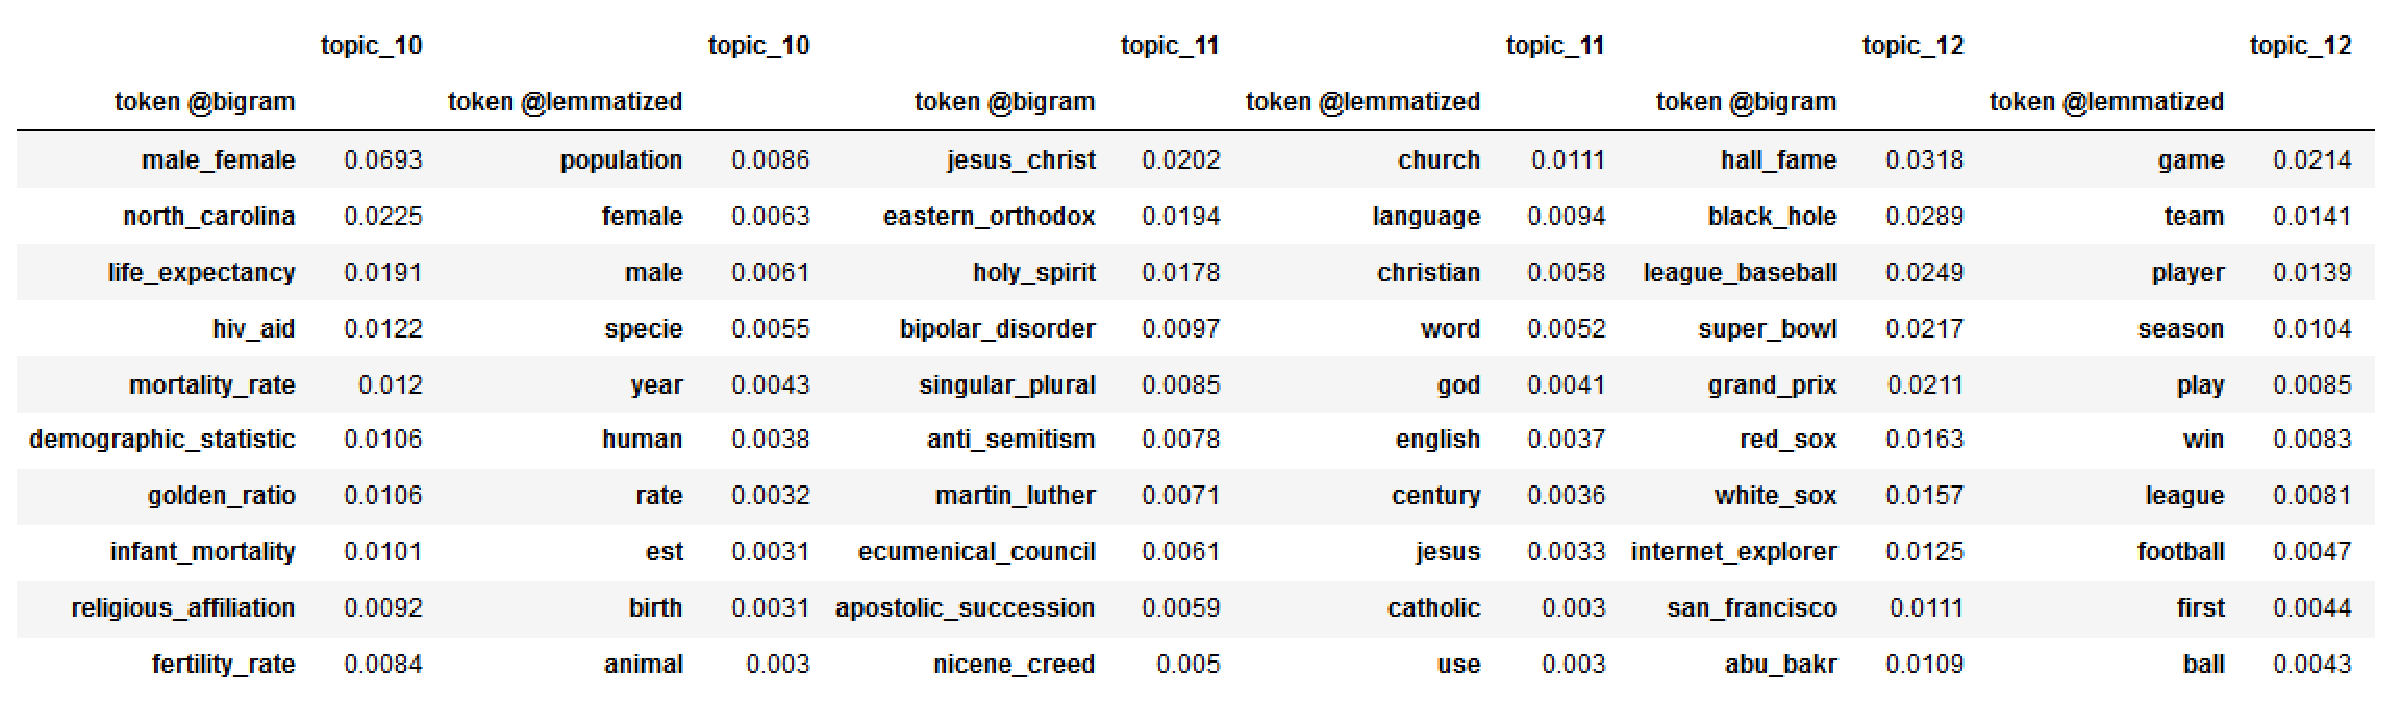
\includegraphics[width=0.98\textwidth]{sorted_3_topics.eps}
    \caption{Output of the TopTokensViewer. Token score in the topic is calculated for every token, score function can be specified at the stage of a viewer initialization.}
\label{top_tokens}
\end{figure*}

\begin{figure}[h]
    \centering
    \includegraphics[width=0.5\textwidth]{cluster_plot.eps}
    \caption{Visualisation of reduced document embeddings colored according to their topic made by DocumentClusterViewer.}
\label{documents_clusters}
\end{figure}

% Examples? common tasks such as TopTokenViewer and TopDocumentViewer and more sophisticated ones like SimilarDocumentViewer, TopicSpectrumViewer

% The library supports a variety of visualisation tools both conventional, such as top tokens and top documents viewers, and experimental ones.

Модуль \texttt{Cooking Machine} содержит различные инструменты для моделирования, 
embodied in the semi-hierarchical structure of the main modelling classes. 
These classes are responsible for building and training model of the given structure, for selecting models according to various constraints and for saving, loading and logging through the modelling process.

Following our ``convention over configuration'' principle, we enforce some assumptions on which kind of experiments TopicNet supports. 
Мы исходим из допущения о том, что процесс построения тематической модели представим в виде дерева. Каждый узел дерева содержит в себе тематическую модель, а ориентированные рёбра хранят информацию об отношениях ``предок-потомок'' вида ``модель $Y$ была получена из модели $X$ при помощи преобразования $T_{XY}$''. Не все деревья эксперимента являются допустимыми. Мы накладываем ограничения на допустимые преобразования: мы требуем, чтобы все рёбра одного уровня описывали преобразования из одного и того же семейства, различающиеся лишь набором параметров. 

Возможные примеры таких преобразований:

\begin{itemize}
    \item Применить к модели регуляризатор с произвольными параметрами (или изменить параметры существующего регуляризатора)
    \item Запустить процесс обучения модели на какое-то количество итераций
    \item Добавить в текущую модель несколько тем, обнаруженных внутри другой коллекции
\end{itemize}

\begin{figure}[t]
    \centering
    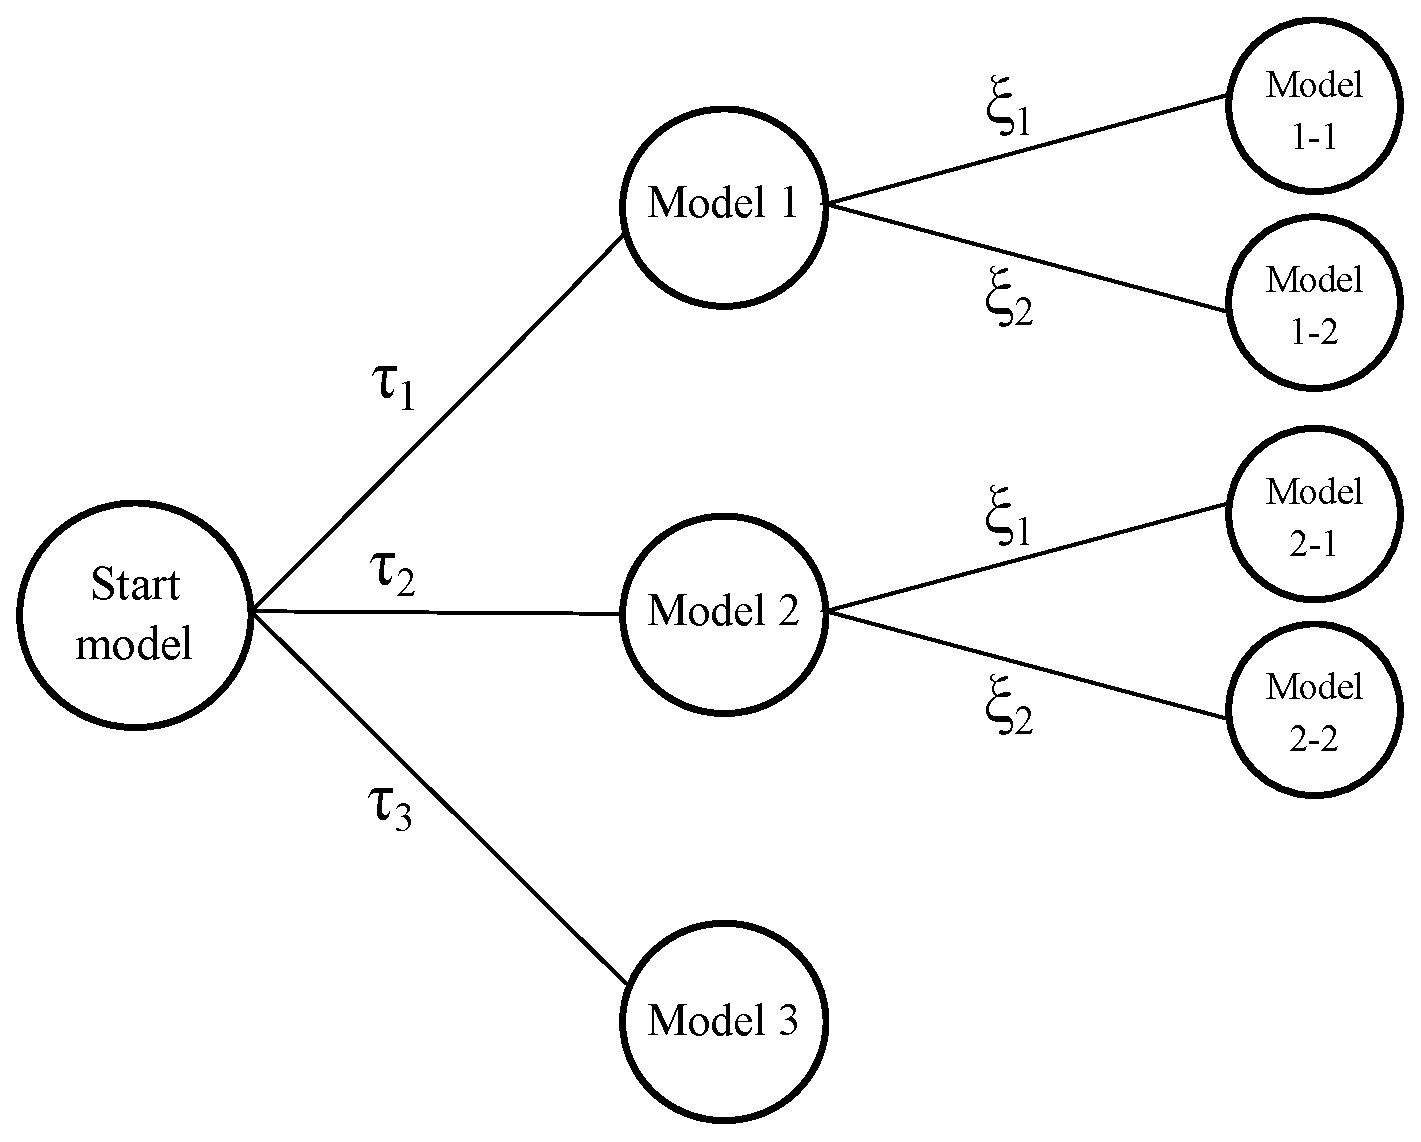
\includegraphics[width=0.4\textwidth]{training_scheme_example.eps}
    \caption{
        Example of the two-stage experiment scheme.
        At the first stage, regularizer with parameter $\tau$ taking values in some range $\{\tau_1, \tau_2, \tau_3\}$ is applied.
        Best models after the first stage are \emph{Model 1} and \emph{Model 2}~---~so \emph{Model 3} is not taking part in the training process anymore.
        The second stage is connected with another regularizer with parameter $\xi$ taking values in range $\{\xi_1, \xi_2\}$.
        As a result of this stage, two descendant models of \emph{Model 1} and two descendant models of \emph{Model 2} are obtained.
    }
\label{Training-scheme}
\end{figure}



Класс \texttt{Experiment} отвечает за хранение, журналирование и актуализацию этой структуры. 

Все преобразования связаны с экземпляром класса \texttt{Cube}. Каждый \texttt{Cube} играет роль чертежа, задающего все преобразования на текущем уровне эксперимента. Таким образом, процесс обучения можно представить как цепочку кубов, последовательно соединённых друг с другом.

Куб выполняет две важные функции. Первая --- это \textit{спецификация}: во время инициализации куб преобразует заданные пользователем параметры в многомерное пространство поиска. Вторая функция --- \textit{применение}: получив точку в пространстве поиска и тематическую модель, куб изменяет какое-то количество параметров и/или гиперпараметров модели. Таким образом, он играет роль инкубатора для моделей, что отражено в названии класса. На Рис.  \ref{Training-scheme} приведена схема обучения, состоящая из двух кубов, применённых к одной модели.

Классы \texttt{Experiment} и \texttt{Cube} позволяют сделать логгирование и сложные стратегии обучения более сжатыми и доступными. Модуль \texttt{config\_parser} делает ещё один шаг в сторону облегчения конфигурируемости: стратегию обучения можно задать при помощи текстового конфигурационного файла в формате YAML.


\section{Механизм отбора моделей в TopicNet}

\begin{figure*}[!ht]
\footnotesize
\texttt{TopicKernel@word.average\_contrast > 0.95 * MAXIMUM(TopicKernel@word.average\_contrast) \\
\hphantom{\ \ } and PerplexityScore@all < 1.1 * MINIMUM(PerplexityScore@all) \\
\hphantom{\ \ } and SparsityPhiScore@word -> max\\
\hphantom{\ \ } COLLECT 3}
\caption{This expression returns three models which are in the top 5\% according to contrast, has acceptable perplexity and as sparse as possible. \texttt{SparsityPhiScore} stands for the fraction of zeros in $\phi_{wt} = p(w \mid t)$ distribution.}
\label{DSL-example}
\end{figure*}

Другая область, описываемая пользователями как громоздкая и непрозрачная --- отбор моделей. В реальных экспериментах не у каждой модели есть потомки; большинство моделей отбрасываются в соответствии с каким-то критерием. Самый естественный, но в то же время самый трудозатратный способ --- это ручное изучение список верхних токенов и верхних документов, на основании которого пользователь принимает решение, какие из моделей являются ``удовлетворительными''. Другой подход заключается в сравнении численных показателей; обычно используется перплексия и когерентность. Библиотека \mbox{BigARTM} добавляет к их числу ещё какое-то число дополнительных метрик: например, разреженность, чистота и контраст \cite{voron15mlj}.

Библиотека TopicNet также поддерживает пользовательские критерии качества. Значительная часть мер, описанных в \ref{chap:metrics}, реализована на платформе TopicNet.

Для того чтобы облегчить груз ручной инспекции, мы реализовали простой domain-specific язык для отбора моделей (пример приведён на Рис \ref{DSL-example}). Результатом этого становится более простой и прозрачный процесс отбора моделей, способный учитывать множество критериев одновременно.

В рамках описываемого подхода каждый критерий отбора моделей представляет собой строку текста на языке, который может быть задан следующей контекстно-свободной грамматикой:

\begin{lstlisting}
S -> <Expr> | <Expr> <Clct>
<Clct> -> COLLECT <Int>
<Expr> -> <Expr> AND <Expr>
<Optr> -> less | eq | great
<Expr> -> <Literal> <Optr> <Number>
<Expr> -> <Literal> to MIN | <Literal> to MAX
<Literal> -> <ScoreName> | model<ParameterName>
\end{lstlisting}

Будем называть выражения вида 
\lstinline{<Literal> <Optr> <Number>} \textit{требованиями}, а выражения вида \lstinline{<Literal> to MIN} и \lstinline{<Literal> to MAX} --- \textit{критериями}. \textit{MIN} и \textit{MAX} задают направление улучшения (вернуть модель с наименьшим либо с наибольшим значением).

Здесь \lstinline{<Int>} обозначает любое неотрицательное целое число, а \lstinline{<Number>} может быть целым числом, дробным числом, либо арифметическим выражением, использующим специальные функции \texttt{MINIMUM}, \texttt{MAXIMUM}, \texttt{AVERAGE}, \texttt{MEDIAN}. 

Символ \lstinline{<ScoreName>} означает имя критерия качества (скора модели, например разреженности), а \lstinline{<ParameterName>} --- свойство тематической модели (например, число тем: \texttt{model.num\_topics}). Требования, содержащие \lstinline{<ParameterName>}, будем называть \textit{структурными требованиями}.

Специальные функции \texttt{MINIMUM}, \texttt{MAXIMUM}, \texttt{AVERAGE}, \texttt{MEDIAN} применяются к \lstinline{<Literal>} (например, \texttt{MINIMUM(model.num\_topics)} или \texttt{MEDIAN(SparsityThetaScore)}). В процессе программной обработки эти функции заменяются на их численные значения, что позволяет использовать требования вида \texttt{SparsityPhiScore\@word > MEDIAN(SparsityPhiScore\@word)} наряду с более простыми \texttt{SparsityPhiScore\@word > 0.8}. 

Сам процесс отбора происходит в несколько этапов. Сначала выбираются все модели, удовлетворяющие заданным структурным требованиям (если структурных требований не задано, то выбираются все модели). Затем по полученной выборке рассчитываются значения специальных функций, после чего на основании не-структурных требований формируется следующий набор моделей. Если критерий отбора не задан, то этот набор просто возвращается пользователю.

Если же критерий отбора задан, то этот набор упорядочивается согласно этому критерию. Если 
имеется дополнительная клауза \texttt{COLLECT N}, то результатом работы будут $N$ наилучших моделей; иначе считается, что $N=1$. 

\section{Сравнение с конкурентами}

Сравнение TopicNet с другими фреймворками затрагивает несколько важных аспектов. Во-первых, было нужно убедиться в том, что обучение одной модели не занимает слишком много времени и не требует слишком много ресурсов. Во-вторых, нужно оценить интерпретируемость и различность тем у каждой модели.

Эксперименты проводились на коллекции 20 newsgroups. По набору 10 верхних токенов каждой темы измерялись две характеристики: 
\begin{itemize}
    \item Umass-когерентность, показывающая согласованность слов между собой. Измерение производилось при помощи сервиса Palmetto \footnote{\url{palmetto.aksw.org/palmetto-webapp} } \cite{roder2015exploring}. В предыдущих работах было показано, что когерентность коррелирует с интерпретируемостью тем \cite{mimno2011}.
    \item Коэффициент подобия Жаккара, показывающий различность полученных тем. Коэффициент подобия, равный нулю, означает что в верхних словах тем нет общих слов (то есть множества их верхних 10 токенов не пересекаются), а равенство его единицы означает, что все темы являются полными дубликатами.
\end{itemize}

\subsection{Использование ресурсов}

Использование вычислительных ресурсов является фактором, который может затруднить широкое распространение фреймворка (например, студенты могут не иметь доступа к большим вычислительным мощностям; промышленное  использование также требует высокой скорости работы и низкой нагрузки на машину). Это сравнение будет проводиться на более крупном датасете NIPS \cite{mccallum1996bow}. 
 
\begin{table}[h]
\begin{tabular}{|l|l|l|}
\hline
                      & \multicolumn{1}{c|}{RAM, MB} & \multicolumn{1}{c|}{Training time, s} \\ \hline
TopicNet              & 991                         & 222.6 (15)                             \\ \hline
TopicNet multiprocess & 1084                        & 51.4 (15)                              \\ \hline
Gensim LDA            & 3559                        & 282.3 (3)                              \\ \hline
STTM DMM              & 3202                        & 52997 (1)                              \\ \hline
STTM PTM              & 1604                        & 84677 (1)                              \\ \hline
STTM WNTM             & 18663                       & 157819 (1)                             \\ \hline
\end{tabular}
\caption{In the first column we consider all the memory taken by the process during the training. The second column represents time needed to complete the training and number of models trained during the session.}
\label{performance-benchmark}
\end{table}

Как видно из таблицы \ref{performance-benchmark}, даже однопоточная версия превосходит конкурентов в скорости; испоьзование нескольких процессоров незначительно увеличивает расход оперативной памяти, но намного ускоряет процесс обучения. Таким образом, TopicNet не добавляет слишком много дополнительных накладных расходов по сравнению с чистой библиотекой BigARTM.

\subsection{Model Quality} 

Следуя изложенным выше целям, мы предоставляем рецепт \texttt{ARTM baseline}, предназначенный для первого знакомства с библиотекой. Чтобы проверить качество этого рецепта, мы сравним модель, полученную посредством рецепта \texttt{ARTM baseline} с моделями ``по умолчанию'' из других фреймворков. Модели LDA и STTM были построены на 20 темах, модель TopicNet состояла из 19 предметных тем и одной фоновой. Никакой дополнительной настройки гиперпараметров не производилось (код тренировки модели приведён на \ref{topicnet_baseline}). 

% for TopicNet model we set 19 topics and one ``background'' topic, which has a special set of regularizers to collect polythematic documents. 


\begin{figure}[!ht]
    \centering
    \includegraphics[width=0.4\textwidth]{topicnet_baseline.eps}
    \caption{Example of the TopicNet baseline experiment.}
\label{topicnet_baseline}
\end{figure}

\begin{table}[h]
\begin{tabular}{|l|l|l|}
\hline
           & \multicolumn{1}{c|}{\begin{tabular}[c]{@{}c@{}}Jaccard measure\\ of topic dissimilarity\end{tabular}} & \multicolumn{1}{c|}{\begin{tabular}[c]{@{}c@{}}Average topic\\ coherence\end{tabular}} \\ \hline
TopicNet   & \textbf{0.00169}                                                                                               & -2.551                                                                                 \\ \hline
Gensim LDA & 0.01374                                                                                               & -2.747                                                                                 \\ \hline
STTM DMM   & 0.37541                                                                                               & -2.726                                                                                 \\ \hline
STTM PTM   & 0.02485                                                                                               & \textbf{-2.510}                                                                                 \\ \hline
STTM WNTM  & 0.01997                                                                                               & -3.572                                                                                 \\ \hline

\end{tabular}
\caption{Topic quality comparison}
\label{topic-comparisson}
\end{table}

Как мы видим из таблицы \ref{topic-comparisson}, построенная TopicNet модель  оказывается на втором месте по интерпретируемости (рис. \ref{topics_distribution} показывает дополнительную информацию о когерентности) и на первом месте по критерию различности тем. Это объясняется регуляризатором декорреляции, используемом в рецепте \texttt{ARTM baseline}. Комбинация этого регуляризатора, используемого скора и механизма, следящего за повышением перплексии, позволила найти модель, удовлетворяющую несколько требований одновременно.

\begin{figure}[!ht]
    \centering
    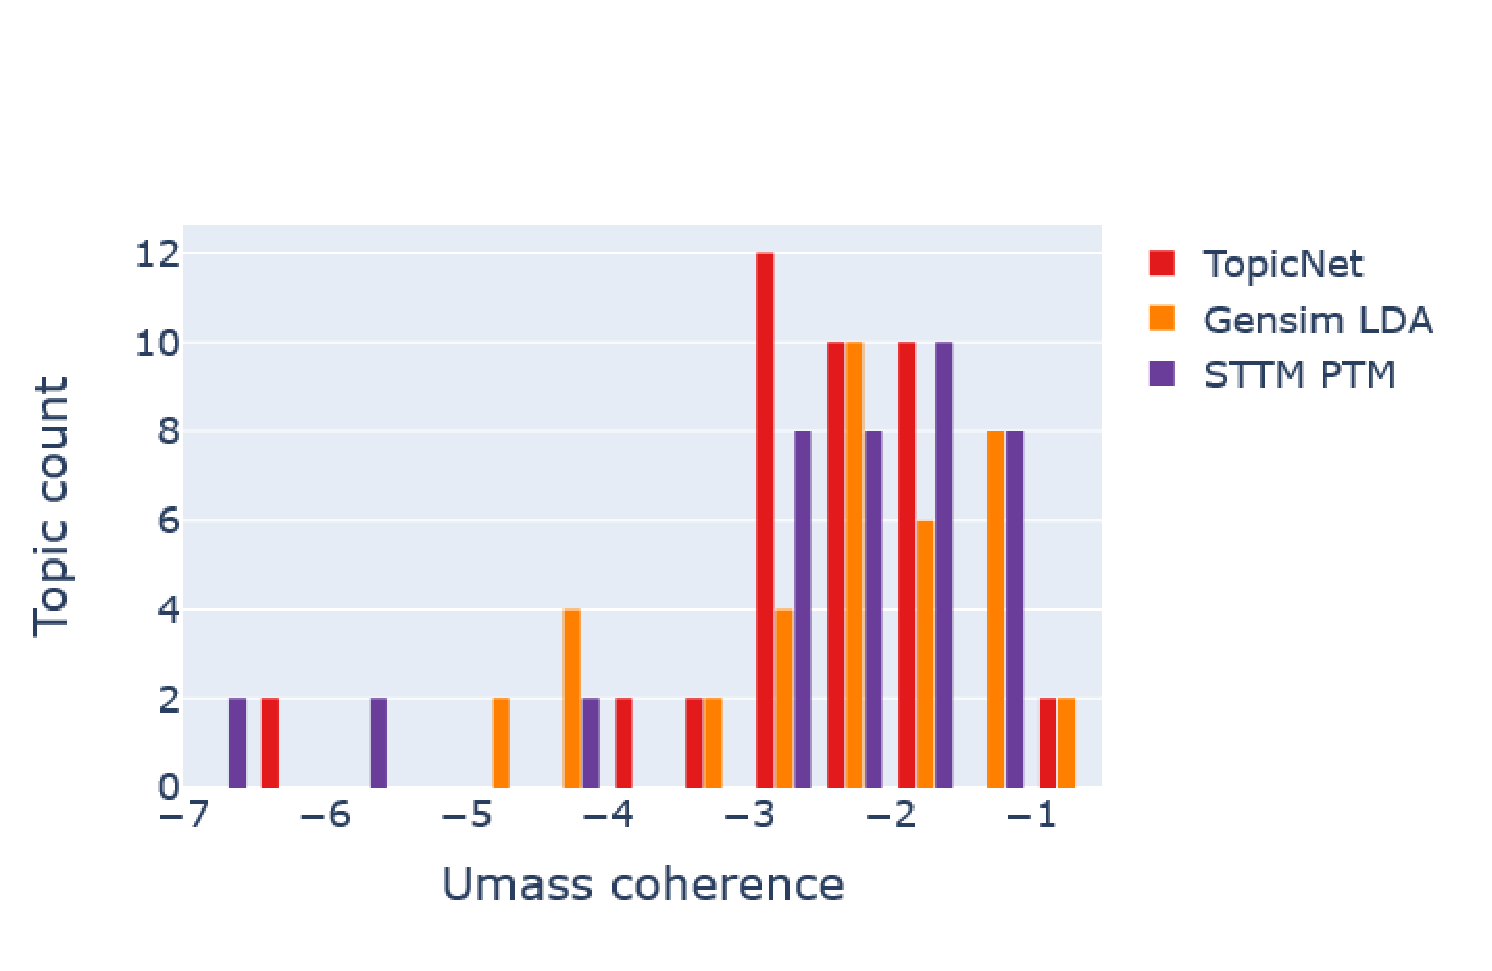
\includegraphics[width=0.45\textwidth]{Topics.eps}
    \caption{Распределение когерентности тем.}
\label{topics_distribution}
\end{figure}

\subsection{Использование псевдорегуляризатора быстрой векторизации}

Во второй серии экспериментов проводилось более детальное сравнение TopicNet с GenSim на той же коллекции.

У GenSim есть несколько режимов запуска, которые можно описать как <<параметры по умолчанию>>. 

Величина $\alpha_{td}$, задающая априорное распределение на $\Theta$, может принимать значения \texttt{asymmetric}, \texttt{symmetric}, \texttt{auto}. Аналогичные значения (кроме \texttt{asymmetric}) может принимать и величина $\eta_{wt}$, задающая априорное распределение на $\Phi$. 

В GenSim инициализация LDA симметричным и/или асимметричным способом задаёт фиксированный численный вектор. Опция \texttt{auto} ведёт себя иначе: параметры распределения Дирихле будут обновляться в процессе обучения модели при помощи метода Ньютона \cite{huang2005maximum}. 

Эти шесть моделей на базе GenSim будут сравниваться с тремя моделями, полученными средствами библиотеки TopicNet. Первая модель --- результат работы рецепта \texttt{BaselineRecipe} (в котором настраивалось только число тем):

\begin{itemize}
    \item Количество тем в модели: 20 предметных, 1 фоновая; 
    \item Два регуляризатора сглаживания фоновых тем по $\Phi$ и $\Theta$ с относительным коэффициентом $\tau=0.1$; 
    \item Регуляризатор декоррлеяции с неизвестным относительным коэффициентом $\tau$ воздействует на предметные темы;
    \item Перебор коэффициента декорреляции $\tau$ производится при помощи \texttt{RegularizersModifierCube} с шагом $0.01$ (стартовое значение $0$, остановка происходит, если перплексия текущей модели более чем а $5\%$ превосходит перплексию модели с $\tau=0$);
    \item Критерий отбора модели: \texttt{PerplexityScore@all < 1.05 * MINIMUM(PerplexityScore@all) and BleiLaffertyScore -> max}. 
\end{itemize}

Результатом этого процесса является тематическая модель с коэффициентом декорреляции $\tau=0.09$. Две другие модели строились аналогично, но с добавлением псевдорегуляризатора быстрой векторизации и с другими критерием отбора: у одной из них также максимизировался \texttt{BleiLaffertyScore}, у другой максимизировался \texttt{LogLift}. Полученные коэффициенты декорреляции равны $0.04$ для \texttt{BleiLaffertyScore} и $0.04$ для \texttt{LogLift} соответственно (заметим, что для \texttt{BaselineRecipe} оба критерия отбора дают одинаковый результат).

Результаты эксперимента приведены в таблице \ref{tab:better_baseline}. Для моделей на базе TopicNet приводятся значения, усреднённые по 20 предметным темам, а для моделей из GenSim --- усреднённые по всем 20 темам. Видно, что комбинированная модель превосходит LDA по всем мерам качества.

\begin{table}[]
\begin{tabular}{lll}
                         & UMass-когерентность & LogLift             \\
BaselineRecipe           & -3.145         & 29.217         \\
ThetalessBleiLafferty   & -2.075         & 31.143           \\
ThetalessLift           & \textbf{-1.805}  & \textbf{33.904} \\
LDA\_asymmetric\_symmetric & -2.446          & 21.388           \\
LDA\_asymmetric\_auto      & -3.078          & 24.321          \\
LDA\_symmetric\_symmetric  & -2.884          & 23.554         \\
LDA\_symmetric\_auto       & -2.279         & 21.738          \\
LDA\_auto\_symmetric       & -2.382           & 24.154          \\
LDA\_auto\_auto            & -2.749          & 25.458        
\end{tabular}
\label{tab:better_baseline}
\caption{Сравнение моделей по ряду метрик качества}
\end{table}


% короче thetaless + фоновые темы с дефолтными параметрами + decorrelation бьёт генсимовский ЛДА и просто фоновую декорреляцию по лифту, когерентности на внешнем корпусе, различности тем

% хотя почему-то проигрывает просто фоновой декорреляции по ppmi (в pmi лучше)


\section{Адаптивная траектория регуляризации}
% не имеющая прямых аналогов в байесовом выводе
% есть alpha_iter но не всегда достаточно гибкости

Адаптивная траектория регуляризации --- мощная техника, находящая себе множество практических применений. Её идея состоит в том, чтобы заменять постоянный коэффициент регуляризации $\tau$ на функцию, зависящую от номера итерации обучения $\tau_i$ (и, возможно, от каких-то характеристик модели). Последовательность $\tau_i$, рассмотренных в процессе обучения, называется \textit{траекторией регуляризации}.

Самый распространённый вариант этой техники --- последовательное включение в модель новых регуляризаторов (может быть вместе с отключением старых регуляризаторов). Последовательное применение куба \texttt{RegularizerModifierCube}, включающих и выключающих определённый регуляризатор, позволяет удобным образом реализовать эту технику внутри TopicNet.

Однако существует и более продвинутый вариант : изменение коэффициента регуляризации
Существуют и более продвинутые использования этой техники. В качестве примера можно привести следующую цитату из \cite{plavin}:

<<Коэффициент декорреляции линейно растет во время первых
60 итераций обучения до наибольшего значения $\gamma = 200000$, не ухудшающего модель. После 15-й итерации включается регуляризатор отбора тем с $\tau=0.3$. Отбор тем и декоррелирование происходит не одновременно, а на чередующихся итерациях (поскольку их эффекты могут конфликтовать)... 

Для того, чтобы избавиться от несущественных слов в темах и подготовить несущественные темы к дальнейшему их устранению, начиная с 40-й итерации включается разреживание. Его коэффициенты постепенно увеличиваются до значений, каждую итерацию обнуляющих $2\%$ элементов $\Theta$ и $9\%$ элементов $\Phi$.>>

Описанная здесь методология иллюстрирует сразу несколько сценариев применения:

\begin{itemize}
    \item Рост до ухудшения: коэффициент регуляризации увеличивается до тех пор, пока перплексия модели держится в допустимом интервале.
    \item Плавное включение: вместо того, чтобы вводить в модель новый регуляризатор с заданным $\tau$, коэффициент постепенно растёт до искомого значения. Используется, если конечное значение коэффициента уже известно.
    % \item Включение с эмпирически подобранной итерации: 
    \item Чередование: например, включение одного набора регуляризаторов на чётных итерациях, а какого-то другого на нечётных. В некоторых случаях позволяет снизить конкуренцию разных регуляризаторов.
\end{itemize}

Каждый из этих сценариев сложно реализовать средствами \texttt{RegularizerModifierCube}. В этой секции будет описан \texttt{RegularizationControllerCube} --- куб, позволяющий работать со сложными траекториями регуляризации.

\subsection{Ухудшение модели}

Для дальнейшего изложения нам необходимо формализовать фразу <<без заметного увеличения перплексии>>. На практике часто используются какой-либо из следующих двух способов определить, что модель адекватно описывает коллекцию: 

\begin{enumerate}
    \item Численное сравнение перплексии с моделью-образцом (например, PLSA). Модель считается допустимой, если её перплексия больше образцовой не более чем на какой-то порог (например, $5\%$).
    \item Визуальный осмотр графика перплексии от номера итерации. Если зависимость выглядит монотонно уменьшающейся, то процесс обучения считается корректным: у модели получается настраиваться и под коллекцию, и под требования регуляризаторов.
\end{enumerate}

Первый подход реализован в рамках \texttt{RegularizerModifierCube}, который поддерживает стратегии оптимизации. В нашем же случае более целесообразным представляется второй подход, не требующий выделения референтной модели.

Предлагается следующий алгоритм анализа изменения перплексии. Пусть $\epsilon$ --- некий заданный порог (например, $5\%$), а  $p(i)$ --- значение перплексии на $i$-ой итерации, $0 < i < n$. Найдём такое $i_0$, что $p(i) \geq p(i_0)~\forall i$. Далее проверим, что $p(i) < (1 + \epsilon) p(i_0)$ при $i > i_0$; если это справедливо, то будем считать модель адекватно настроившейся под данную коллекцию.  

Опишем интуицию, стоящую за этим алгоритмом. Поскольку $p(i_0)$ является глобальным минимумом, то точка $i_0$ разделяет график $p(i)$ на левую и правую части: $p(i) \geq p(i_0)$ при $i < i_0$, и $p(i) \geq p(i_0)$ при $i > i_0$. Это отражает типичное поведение перплексии при обучении: сначала резкий спад, затем, возможно, увеличение (не обязательно монотонное). Увеличение считается заметным, если его максимальное значение превосходит $p(i_0)$ более чем в допустимые $(1 + \epsilon)$ раз.

\subsection{Архитектура Regularization Controller Cube}

Модуль определяет вспомогательный класс
\texttt{ControllerAgent}. Экземпляр этого класса связан с конкретным регуляризатором конкретной модели и хранит в себе следующие поля:

\begin{itemize}
    \item \textbf{Имя регуляризатора}, коэффициент \texttt{tau} которого будет регулироваться.
    \item \textbf{Имя скора} (\texttt{score\_to\_track}), по изменениям которого будет проверяться ухудшение модели. Подразумевается, что это идентификатор переплексии для определённой модальности (или их совокупности). 
    \item \textbf{порог}, который обозначен выше как $\epsilon$ (по умолчанию --- $5\%$).
    \item \textbf{Максимальное число итераций}, по истечении которого текущий Controller Agent  прекратит регулировать коэффициент регуляризации. Может быть равно бесконечности, по умолчанию равно полю \texttt{max\_iters} у  \texttt{RegularizationControllerCube}, отвечающего за этот этап обучения.
    \item \textbf{Диапазон пользовательских значений} (\texttt{user\_value\_grid}): список численных значений. Этот параметр не несёт самостоятельной семантики; его смысл определяется функцией \texttt{tau\_converter}.
    \item \textbf{Функция преобразования} (\texttt{tau\_converter}): заданная пользователем функция, преобразующая $\tau$ с предыдущей итерации в $\tau$ для текущей итерации (может задаваться как функция или как строка). У функции четыре входных аргумента: 
    \begin{itemize}
        \item \texttt{initial\_tau}: значение $\tau$ в начале применения куба,
        \item \texttt{prev\_tau}: значение $\tau$ с предыдущей итерации,
        \item  \texttt{cur\_iter}: номер текущей итерации,
        \item \texttt{user\_value}: пользовательское значение (элемент списка \texttt{user\_value\_grid}).
    \end{itemize}
\end{itemize}

Также Controller Agent хранит в себе историю изменений коэффициента $\tau$ и историю изменений метрики качества \texttt{score\_to\_track}. История метрики качества проверяется каждую итерацию по описанной выше схеме; если ухудшения метрики считаются допустимыми, то коэффициент регуляризации обновляется по пользовательской формуле. В противном же случае коэффициент 
откатывается к предыдущему безопасному значению и больше не меняется (Controller Agent отмечается как выключенный).

Применение куба сводится к запуску перебора по сетке: если \texttt{user\_value\_grid} состоит из $K$ чисел, то создаётся $K$ моделей, каждая из которых имеет свой индивидуальный user value.

В таблице \ref{tab:controller_examples} приведены примеры использования описываемого здесь Regularization Controller Cube.

\begin{table}[]
\small
\begin{tabularx}{\textwidth}{ZcZ}
Выражение                                                      & Сетка пользовательских значений  & Смысл                                                                                       \\ \hline
\texttt{initial\_tau} 
\texttt{if cur\_iter \% 2 == 0} 
\texttt{else 0}            & [0, 0.01, 0.02, 0.05]            & Чередование                                                                                 \\ \hline
\texttt{prev\_tau + user\_value}                                 & [50, 100, 150, 200, 250]         & Линейное возрастание коэффициента \\ \hline
\texttt{user\_value * (cur\_iter - 8)} 
\texttt{if cur\_iter > 8} 
\texttt{else 0} & [0, 0.01, 0.02, 0.05]            & Линейное возрастание коэффициента, начиная с восьмой итерации \\ \hline 
\texttt{prev\_tau * user\_value}                               & [1, 0.95, 0.90, 0.80, 0.5] & Экспоненциальное затухание коэффициента % (с неизвестным <<периодом полураспада>>) 
\\ \hline
\texttt{prev\_tau * user\_value}                               & [1, 1.1, 1.5, 2]                 & Мультипликативное возрастание коэффициента    \\ \hline
\texttt{50 * (cur\_iter - user\_value)} 
\texttt{if cur\_iter > user\_value} 
\texttt{else 0}   & [10, 15, 20, 25, 30]             & Линейное возрастание коэффициента, начиная с итерации с неизвестным номером \\ \hline
\texttt{initial\_tau} 
\texttt{if cur\_iter < user\_value} 
\texttt{else 0}        & [10, 15, 20, 25, 30]             & обучение с регуляризатором $N$ итераций, 
затем обучение без регуляризатора оставшееся число итераций \\ \hline             
\end{tabularx}
\label{tab:controller_examples}
\end{table}


% скорее коэффициент регуляризации откатывается к предыдущему значению, а модель уж как получилось.
% это такой damage control, который пытается сделать так, чтобы модель находилась в опасной зоне не больше одной итерации





\section{Заключение}
В этой главе был описан гибкий, конфигурируемый и быстрый фреймворк для подбора параметров и построения тематических моделей; показаны его преимущества по сравнению с другими фреймворками. TopicNet предоставляет широкий функционал: построение моделей с нуля, создние пользовательских скоров и регуляризаторов, возможность настройки параметров ранее построенных моделей.

Библиотека предоставляет готовые рецепты, отражающие лучшие практики построения АРТМ моделей под конкретную цель. Как было показано ранее, аддитивно регуляризованная модель способна превзойти модели конкурентов в терминах согласованных и не-повторяющихся тем. TopicNet помогает улучшить регулризованные модели дальше за счёт возможности введения пользовательских регуляризаторов и настройки гиперпараметров для мультикритериальных задач. 

При помощи комбинации BigARTM и TopicNet неспециализированный пользователь может реализовать новую тематическую модель, не встречавшуюсся в литературе раньше (другие фреймворки не позволяют этого добиться).

Помимо инструментов для гибкого и быстрого тематического моделирования, библиотека предоставляет средства контроля качества построенных моделей. TopicNet позволяет оценивать модели посредством различных встроенных метрик (скоров) и даёт возможность задать произвольные пользовательские метрики. Скоры могут вычисляться каждую итерацию тренировки, только на последней итерации, или с каким-то периодом. 

Также в состав библиотеки входит набор инструментов визуализации. К их числу относятся традиционные (top tokens and top documents viewers) и экспериментальные (спектр).

Библиотека TopicNet --- программный проект с открытым исходным кодом, имеющий потенциал для дальнейшего расширения. Модули \texttt{viewers} и \texttt{cooking machine} были спроектированы с учётом возможных улучшений со стороны сообщества в будущем.

Эти особенности дают основания верить в то, что эта библиотека будет одинаково полезна для software engineers и исследователей в области digital humanities.

           % Глава 3
\chapter{Применение регуляризации для кластеризации интентов}

В данной главе предлагается иерархическая мультимодальная регуляризованная тематическая модель, играющая роль первого приближения к структуре коллекции. Главное достижение, описанное в этой главе, --- построение двухуровневой иерархической тематической модели, использующей различные признаки на первом и втором уровнях. Насколько нам известно, ранее в литературе подобный подход не изучался.  Вводится специфичная для задачи мера качества, измеряющая качество иерархических связей между темами и обнаруженными интентами.

Иерархическая структура увеличивает интерпретируемость предлагаемой кластеризации. Точнее говоря, от тем первого уровня требуется, чтобы они описывали субъект диалога, а темы второго уровня должны описывать действие, в котором заинтересован пользователь. Информация о частях речи слов используется для того, чтобы достичь этой цели.

\section{Предобработка} \label{nlp_methods}

Для двух описанных далее коллекций использовалась одна и та же процедура предобработки. Она состоит из большого числа частей (поэтому важно, чтобы каждая из них была сравнительно быстрой), описанных ниже.

\textbf{Первичная обработка данных}: очистка от ненужной информации. В её состав входит:

\begin{itemize}
    \item  \textbf{Фильтрация документов}. Удаление длинных документов, часто встречающихся в качестве сообщений (например, автоматические сообщения — <<Создано новое обращение \#123>>).
    \item \textbf{Выделение/удаление простых сущностей}. Выделение URL-адресов, html-тегов, адресов электронной почты. Каждая сущность заменяется на свой тег: например, все гиперссылки заменяются на <URL>. Для каждой из сущностей задан набор регулярных выражений.
\item \textbf{Выделение/удаление географических локаций}. Выделение городов и регионов. Выделение происходит с помощью поиска по некоторому списку географических локаций.
\item \textbf{Посимвольная нормализация}. Удаление повторяющихся знаков пунктуации. Замена нескольких повторяющихся знаков пунктуации на один знак. Замена ё на е. Удаление повторяющихся пробелов.
\item \textbf{Исправление раскладки}. Если в тексте содержится несколько слов не из словаря, которые при смене раскладки будут оказываться в словаре, раскладка всего текста изменится.
\item \textbf{Исправление опечаток}. Опечатки исправляются двухэтапно. Для каждого слова в предложении генерируются кандидаты на исправление, затем из всех кандидатов выбирается лучший с помощью языковой модели. Теоретически алгоритм способен исправлять ошибки: пропущено две буквы, добавлено две лишних буквы, два раза две буквы поменялись местами, слились два соседних слов в одно. Далее процесс исправления опечаток будет рассмотрен более подробно.
\end{itemize}

Нормализация данных:

\begin{itemize}
\item \textbf{Токенизация}. Токенизация документов (разделение на отдельные токены) с помощью библиотеки spacy. Сначала документ разделяется на токены по любым символам, которые не являются буквой или цифрой. Затем, согласно специальным шаблонам, некоторые группы токенов соединяются вместе.
\item \textbf{Выделение/удаление имён/фамилий}. Выделение имён и фамилий. Производится с помощью библиотеки pymorphy2.
\item \textbf{Лемматизация}. Лемматизация документов (приведение всех слов в начальную форму) с помощью библиотеки pymorphy2.
\item \textbf{Учёт частицы не}. Склеивание не со следующим словом, если слово является глаголом (таким образом, тематическая модель может отличить <<получается>> от <<не получается>>).
\item \textbf{Выделение информативных $n-$грам}. Выделение $n-$грам (коллокаций или устойчивых словосочетаний) с помощью алгоритма TopMine. Далее этот этап будет рассмотрен более подробно.
\item \textbf{Удаление стоп-слов}. Удаление стоп-слов по заранее заданному списку слов и списку регулярных выражений.
\item \textbf{Разделение данных на группы}. Разделение слов и словосочетаний на две группы: “тематичные/предметные” и “функциональные”. Процедура и смысл этого разделения будут описаны ниже.
\end{itemize}

\subsection{Объединение и фильтрация реплик}

Дополнительно происходит фильтрация некоторых реплик, определённых как “мусорные”. Обычно это дословный copy-paste текста какого-либо нормативного документа или содержимого веб-страницы (в том числе и предыдущего диалога).

Обучение кластеризации на таких объектах снижает итоговое качество модели. Кроме того, становится неудобно изучать выдачу топ-документов тем. Используются три критерия <<мусорности>> реплики (реплика удаляется, если справедлив хотя бы один из них).

Первым критерием является \textbf{многострочность}. Главными признаками этого критерия считается достаточная длина реплики (больше 6 строк или 10 слов) при малом количестве знаков препинания (каждая строка в среднем содержит менее 2/3 знака).

Данный критерий выделяет содержимое веб-страницы, скопированное в чат. В этом случае перенос строки означает не конец абзаца, а конец структурного элемента страницы; соответственно, отсутствует завершающий предложение знак препинания.

Вторым критерием является \textbf{пропорция одинаковых слов}. Для его проверки сравнивается длина реплики в словах и количество уникальных слов в реплике. Реплика считается мусорной, если каждое уникальное слово встречается в ней больше $2.5$ раз (в среднем). Это правило применяется только к репликам, состоящим более чем из 10 слов.

Критерий позволяет найти реплики, в которых одна и та же фраза повторяется несколько раз.

Третий критерий основан на \textbf{скорости убывания частот слов}. Частотность естественной речи обычно подчиняется закону Ципфа или похожим степенным распределениям; самое частое в тексте слово должно быть в несколько раз более распространённым, чем следующее по частоте.

Для проверки этого критерия все слова сортируются по их числу вхождений в реплику, затем на основании частот трёх самых распространённых слов $w_1~,w_2~,w_3$ вычисляется скорость убывания частоты слов ($\frac{n_{d{w_1}}}{n_{dw_2}}$ и $\frac{n_{d{w_2}}}{n_{dw_3}}$). Реплики, состоящие из одной строки, считаются мусорными, если оба этих отношения не превосходят $1$. Для многострочных реплик оба этих отношения должны быть не меньше $2$.

Расчёт частот идёт без учёта предлогов, местоимений, союзов и цифр. Это правило выделяет реплики, содержащие многократное повторение одной и той же фразы с небольшими изменениями или непохожие на естественную речь. Примером последнего служат тексты песен или текст отчёта об ошибке (error traceback).

После удаления мусорных реплик происходит объединение всех сообщений диалога в один документ. Реплики оператора не учитываются в этом объединении. Таким образом, один документ коллекции --- это конкатенация всех реплик пользователя из одного диалога.

\subsection{Автоматическое выделение $n$-грамм}

\par Распространённая техника, улучшающая интерпретируемость тематических моделей --- использование информативных $n$-грамм, называемых также коллокацийями, в качестве дополнительной модальности. Для того чтобы извлечь информативные нграмы, был использован алгоритм TopMine \cite{topmine}, основанный на статистике совстречаемостей слов.

Для нашей задачи имело смысл внести ряд правок в алгоритм TopMine.

Во-первых, исходный алгоритм вычисляет статистики совстречаемости для упорядоченных кортежей слов $(w_1, w_2, \dots, w_k)$. В частности, алгоритм различает последовательности $(w_1, w_2)$ и $(w_2, w_1)$. Эта особенность делает алгоритм TopMine плохо приспособленными для обработки текстов на языках с нестрогим порядком слов (таких как русский). По этой причине логика подсчёта статистик совстречаемостей алгоритма была модифицирована таким образом, чтобы в ней использовались мультимножества слов вместо последовательностей слов.

Во-вторых, TopMine не выделяет пересекающиеся коллокации. Это приводит к тому, что похожие предложения (<<записать ребёнка в детский сад>> и <<записать ребёнка в детский садик>>) могут вовсе не содержать общих коллокаций. Примером служат предложение <<получение паспорта РФ>> (выделится коллокация \texttt{получение\_паспорт\_РФ}) и предложение <<паспорт РФ был утерян>> (выделится коллокация \texttt{паспорт\_РФ}). Это следует из процесса поиска коллокаций алгоритмом: на каждом шаге обработки соседние коллокации-кандидаты сливаются, если их объединение удовлетворяет критерию информативности. Для того чтобы устранить вышеописанную проблему, достаточно изменить процесс итеративного слияния фраз так, чтобы при успешном слиянии коллокаций они не удалялись из множества кандидатов. Данная модификация увеличивает расход памяти алгоритма, однако делает процесс поиска не <<жадным>>.

\subsection{Распознавание именованных сущностей}

\par В текстах диалогов содержится большое число упоминаний имён участников, названий компаний/продуктов и названий улиц/городов. Аккуратный учёт такого рода сущностей (Named entity recognition) даст прирост качества моделей, а также сделает списки верхних слов более интерпретируемыми (к информативным словам не будут примешиваться имена операторов-собеседников).

Поэтому в рамках предобработки коллекции все обнаруженные именованные сущности заменялись на теги $\langle \mathrm{PERSON} \rangle$.

Рассматривалось несколько подходов к выделению именованных сущностей: с помощью правил/словарей и с помощью использования RNN+CRF модели.

Нейронная сеть из работы \cite{burtsev}, предобученная на датасете PERSONS-1000 (\cite{persona}), давала лучшее качество выделения именованных сущностей. Однако соображениями вычислительной эффективности был продиктован выбор модуля \texttt{pymorphy2} (основанного на правилах) для окончательной версии конвейера предобработки.

\subsection{Коррекция ошибок}

\par Ошибки и опечатки --- частое явление в дилоговых корпусах. Для того чтобы сделать текстовую коллекцию более подходящей для тематического моделирования, необходимо использовать алгоритм коррекции ошибок. В данной работе используется Jamspell\footnote{\href{https://github.com/bakwc/JamSpell}{Jamspell github}} по причине высокой скорости его работы.

\par Был проведён ряд модификаций для того, чтобы адаптировать модель Jamspell к нашему случаю. Во-первых, языковая модель, согласно которой выбирается лучший кандидат для исправления, была дообучена на кластеризуемой коллекции. Эта модификация нужна для учёта специфики коллекции; в противном случае специфичные для коллекции слова (такие как <<гибдд>> или <<адсл>>) считались бы незнакомыми и в них исправлялись бы несуществующие опечатки.

Во-вторых, было расширено множество кандидатов для исправления. Согласно статистике поиска Яндекса\footnote{Сложности русского языка: \texttt{https://yandex.ru/company/researches/2016/ya\_spelling}}, одной из наиболее распространённых категорий ошибок является слитно-раздельное написание слов; в текстах коллекции также часто встречаются <<слипшиесся>> слова (<<\textbf{очередьк} врачу>>). Поэтому все возможные разбиения слова на два также рассматривались как кандидаты на исправление.

\section{Построение модели}
Для кластеризации полученных объектов строится тематическая модель. \par Темы тематической модели, которую мы стремимся построить, должны соответствовать пользовательским интентам. В данной работе используется следующее операциональное определение интента: два диалога (представленные репликами пользователя) считаются \textit{имеющими одинаковый интент}, если оба пользователя были бы удовлетворены практически одинаковой реакцией оператора колл-центра. Это определение, несмотря на свои недостатки, позволяет подчеркнуть ряд важных практических проблем:

\begin{itemize}
\item Простого подхода, основанного на гипотезе <<мешка слов>>, недостаточно. Сравните: <<Я хочу заблокировать свою учётную запись, что мне делать?>> and <<Моя учётная запись заблокирована, что мне делать?>>
\item В некоторых случаях замена одного слова изменяет интент реплики, а в других --- нет. В контексте имеющейся коллекции <<я хочу записаться на приём к кардиологу>> и <<я хочу записаться на приём к неврологу>> считаются одинаковыми интентами, поскольку требующиеся от пользователя/оператора действия практически не отличаются. Однако <<уплата госпошлины за паспорт>> и <<уплата госпошлины за автомобиль>> существенно различаются. 
\end{itemize}

Для того чтобы получить больше контроля над выделением интентов, предлагается двухуровневая иерархическая тематическая модель. Первый уровень предназначен для грубого определения похожести, в то время как второй уровень учитывает менее очевидные, но важные признаки.

Иерархическая АРТМ модель представляет собой набор различных АРТМ моделей для каждого уровня, связанных друг с другом. Первый уровень иерархии может быть любой тематической моделью. Второй уровень строится с использованием специального регуляризатора из работы \cite{chirkova2016additive}, который стремится сделать модель такой, чтобы темы первого уровня выражались через взвешенную сумму тем второго уровня.

Выход иерархической модели — распределение тем первого и второго уровня по словам и документам, а также матрица зависимостей тем второго уровня от тем первого уровня.

Для обеспечения того, чтобы каждая родительская тема была связана лишь с небольшим числом дочерних тем, можно применить различные методы. Обычно используется регуляризатор, разреживающий междууровневые связи \cite{chirkova2016additive} ; также в литературе была предложена процедура прямого удаления <<плохих>> рёбер (в соответствии с мерой качества EmbedSim \cite{belyy}).

\subsection{Построение уровней иерархии} \label{hierarchy_distinct}

Для того чтобы построенные моделью темы второго уровня существенно отличались от тем первого уровня, мы модифицировали признаковое пространство для модели второго уровня.

В контексте поставленной задачи было предпринято разделение признаков по их функциональному назначению. Из всех токенов (слов и нграм) были выделены две группы на основании их частеречного состава: <<тематическая>> и <<функциональная>>. <<Функциональная>> группа состоит из одиночных глаголов и нграм, содержащих хотя бы один глагол. <<Тематическая>> группа состоит из одиночных существительных, одиночных прилагательных и нграмм, включающих в себя хотя бы одно существительное и не имеющих в своём составе глаголов.

Таким образом, предлагаемая тематическая модель имеет пять модальностей: \texttt{@lemmatized} (просто слова), \texttt{@verb\_lemmatized} (слова-глаголы), \texttt{@noun\_lemmatized} (слова-существительные и слова-прилагательные), \texttt{@theme\_ngramms} (нграмы с существительными и без глаголов), \texttt{@verb\_ngramms} (нграмы с глаголами).

% Inspired by multi--level \cite{Tang2018SubgoalDF} and multi--syntactic \cite{Gupta2018SemanticPF} phrases annotation, among with hierarchical partition, our approach is essential for client goal and subgoals extraction.

\par Первый уровень иерархии предназначен для определения субъекта диалога (то есть сущностей, о которых идёт речь). По этим соображениям вес тематической группы токенов должен быть существенно выше, чем вес функциональной группы. Цель второго уровня иерархии --- нахождение интента клиента, касающегосся определённых сущностей (то есть действий, которые пытается предпринять клиент). На этом уровне функциональные токены должны иметь большее влияние, нежели токены тематической группы. Токены модальностей, напрямую не относящихся к данным двум группам, используются на всех уровнях; они выступают в роли связи между двумя разными слоями иерархии.

Сначала строится первый уровень тематической модели, затем второй, так, чтобы любая тема первого уровня являлась линейной комбинацией тем второго уровня. Для каждого из уровней используется свой набор коэффициентов важности категорий признаков (модальностей).
Первый уровень соответствует разделению документов на “темы”, поэтому для построения уровня больший вес имеют “тематичные” признаки: слова-существительные и слова-прилагательные, словосочетания, не содержащие глаголов.
Второй уровень соответствует разделению документов на “интенты”, поэтому для построения второго уровня больший вес по сравнению с первым уровнем имеют признаки: слова-глаголы, словосочетания, содержащие глаголы.
На обоих уровнях для построения кластеризации с небольшим весом используются словосочетания из реплик операторов. Для того чтобы модель была устойчива к разным коллекциям, используются не абсолютные веса для задания значимости категории признаков, а относительные (вес — число от 0 до 1, равный вес у разных категорий означает одинаковую значимость этих категорий для модели).
% На каждом уровне модели используется некоторое количество “фоновых” тем. Эти темы являются техническими, их цель — собирать внутри себя слова фоновой лексики, не влияющие на кластеризацию. К этим темам нельзя получить доступ через систему запросов.
% На каждом уровне модели используется свой набор регуляризаторов со своими коэффициентами регуляризации. Все коэффициенты, за исключением коэффициента регуляризатора декоррелирования (отвечающего за повышение отличия разных тем друг от друга), настраиваются автоматически.

\subsection{Обработка результатов моделирования}

Выход иерархической модели не обязан по построению иметь древовидную структуру (хотя и стремится к ней). Чтобы выход иерархии был древовидным, используются дополнительные преобразования итоговой структуры: для каждой темы второго уровня выбирается единственная тема первого уровня.

Каждую полученную тему можно представить наборами репрезентативных документов и репрезентативных токенов. Над набором документов проводится дополнительная фильтрация: удаляются документы, в которых почти не встречается самых репрезентативных нграмм, удаляются тексты с непропорционально большим количеством заглавных букв.

\section{Эксперименты}

В экспериментах были использованы две коллекции диалогов из русских колл-центров (примерно по 90 тысяч диалогов в каждой, средняя длина диалога --- шесть реплик). Первый корпус состоит из диалогов клиентов с представителями различными государственных организаций. Второй корпус представляет собой логи технической поддержки провайдера. Оба датасета непубличны.

\subsection{Оценка качества}

Существует ряд подходов для оценки качества тематических моделей, в частности их интерпретируемости. Традиционная процедура включает в себя анализ списка верхних слов каждой из тем людьми. Однако данный подход имеет фундаментальные недостатки, о которых было рассказано ранее \ref{chap:coh}. В рамках этой задачи был использован другой подход.
Для каждого датасета были сгенерированы пары $(d_1, d_2)$ (где $d_i$ --- диалог), которые впоследствии были размечены тремя экспертами. Для измерения качества модели полученные таким образом метки сравнивались с метками, полученными из модели.
Приведённый ниже список резюмирует описанный подход к оценке качества и регламент разметки, предложенный экспертам:
\begin{itemize}
    \item \texttt{0}: между $d_1$ и $d_2$ нет ничего общего. В терминах тематической модели такие диалоги должны относиться к разным темам первого уровня.
    \item \texttt{1}: Оба диалога связаны с одним и тем же объектом, но между ними имеются существенные различия. Такие диалоги должны попадать в одну и ту же тему первого уровня, но относиться к двум разным темам второго уровня.
    \item \texttt{2}: Оба диалога $d_1$ и $d_2$ имеют один и тот же интент. Такие диалоги должны относиться к одинаковым темам первого и второго уровня.
    \item \texttt{?}: Невозможно определить интент по крайней мере в одном из рассматриваемых диалогов.
\end{itemize}

Оценка качества моделей производится через измерения точности по этим размеченным парам. Таким образом, отбор моделей происходит по принципам, согласующимся с соображениями, изложенными в \ref{multilevel}.

Разметка разделена на три набора пар: <<1-small<< и <<2-small<< относятся к первой коллекции и состоят из $\sim\!12K$ и $\sim1.5K$ объектов соответственно, а набор <<2-small>> относится ко второй коллекции и состоит из $\sim\!1.5K$ пар. Гиперпараметры модели подбираются исходя из точности, измеренной на  наборе <<1-big<<. Два оставшихся набора (<<1-small<< и <<2-small<<) используются для контроля переобучения. Стоит отметить, что хорошее качество, продемонстрированное на датасете 2-small свидетельствует о том, что стратегия построения модели обобщается на коллекции, отличной от изначальной.



\subsection{Базовые модели}

\par Простейший способ построения модели кластеризации на коллекции текстовых документов состоит из двух этапов. Сначала каждый документ каким-либо образом отображается в вектор действительных чисел. Затем к полученным векторам применяется один из стандартных алгоритмов кластеризации.


\par Существует много способов построить по документу его векторное представление. Простейший из них --- просто кодировка каждого документа вектором длины $W$ (полученный вектор будет равен сумме прямо закодированных (one-hot encoding) векторов для всех составляющих документ слов). Несложная, но действенная его модификация --- замена счётчиков встречаемостей на tf-idf.

Логистическая регрессия, работающая с tf-idf представлениями, показывает достаточно хорошее качество в задачах классификации. Этот алгоритм --- достойная точка отсчёта даже в контексте глубинного обучения \cite{park2019adc}. При этом часто tf-idf представление оказывается неприменимым для задачи кластеризации в силу проклятья размерности. Методы снижения размерности могут помочь решить эту проблему; к их числу относятся PCA и Uniform Manifold Approximation and Projection (UMAP, \cite{mcinnes2018umap}).

\par Другой распространённый подход основывается на векторных представлениях слов \cite{embeddings_in_tm}. Сначала каждому слову ставится в соответствие его векторное представление; представление документа получается через усреднение представлений отдельных слов.

Наиболее распространённые представления слов относятся к семейству word2vec \cite{word2vec}: CBOW, Skip-gram и их модификации (\cite{mikolov2013efficient}).  Подобные модели необходимо обучать на большой коллекции документов, такой как <<Википедия>>. При использовании векторных представлений слов для кластеризации часто применяется снижение размерности \cite{park2019adc} (как и в предыдущем подходе).

Векторное представление документа может быть получено несколькими способами, использующими различные схемы усреднения представлений слов. Помимо арифметического усреднения, в котором вклад каждого слова одинаков, используется усреднение с idf-весами, благодаря которым редкие слова оказывают большее влияние, чем частые.

Использование этих и подобных техник вкупе с тонкой настройкой их параметров позволяет повысить качество кластеризации.

Следующая процедура была использована в качестве первой базовой модели. Сначала тексты были преобразованы в вектора действительных чисел при помощи предобученных представлений либо значений tf-idf. Затем данный набор векторов был прокластеризован при помощи алгоритма K-средних (K-Means). Наконец, каждый полученный кластер разбивается на несколько более мелких (каждый кластер при этом считается отдельной коллекцией). В результате получаются кластера как первого, так и второго уровня.

В роли второй базовой модели выступали иерархические тематические модели: иерархическая тематическая модель без дополнительной регуляризации и иерархическая тематическая модель со сглаживанием распределений  $\Phi$ и $\Theta$ на обоих уровнях.

Количество тем/кластеров на обоих уровнях для базовых моделей настраивались для получения наилучшего качества. Для подхода, основанного на K-Means, дополнительно настраивалась размерность представлений. Как демонстрирует таблица  \ref{baselines}, на двух из трёх размеченных наборах пар регуляризованная тематическая модель превосходит основанный на K-Means подход.

\begin{table}[!h]
    \centering
\begin{tabular}{p{2.7cm}|c|c|c}
    \hline
    & 1-big           & 1-small            & 2-small            \\ \hline
    hKmeans (tf-idf)      & 0.568          & 0.593          & \textbf{0.649} \\
    hKmeans (emb.) & 0.615          & 0.638          & 0.641          \\
    hPLSA         & 0.603          & 0.675          & 0.633          \\
    hARTM         & \textbf{0.636} & \textbf{0.683} & 0.631          \\  \hline
\end{tabular}
    \caption{Baselines accuracy}
    \label{baselines}
\end{table}


\subsection{Качество предложенной модели}

Построение модели происходит последовательно, будут настраиваться как параметры модели, так и этапы конвейера предобработки (описанные в \ref{nlp_methods}). Поиск происходит в следующем порядке:

\begin{enumerate}
    \item Добавление модальности $n-$грам, настройка алгоритма их извлечения, подбор весов модальностей и числа тем;
    \item Добавление регуляризатора сглаживания $p_{tdw}$ на первом уровне иерархической модели, подбор коэффициента регуляризации и числа тем; 
    \item Замена имён на теги, выбор между словарными и нейросетевыми подходами к определению именованных сущностей; 
    \item Исправление опечаток, выбор между стандартным и модифицированным алгоритмом исправления опечаток.  
\end{enumerate}

Отправная точка поиска --- модель hPLSA.

\begin{table}[!h] 
    \centering 
\begin{tabular}{p{2.7cm}|c|c|c} 
    \hline 
    & 1-big            & 1-small            & 2-small            \\ \hline 
    hPLSA         & 0.603          & 0.675          & 0.633          \\ 
\hline \hline 
    + n-grams стандарт & 0.612 & 0.634 & 0.633 \\ 
    + n-grams модификация & \textbf{0.635} & \textbf{0.674} & \textbf{0.655} \\ 
\hline \hline 
    + сглаживание ptdw & \textbf{0.64} & \textbf{0.678} & \textbf{0.66} \\ 
\hline \hline 
    + NER по словарю & 0.634         & 0.661         & 0.635 \\ 
    + NER через нейросети & \textbf{0.64} & \textbf{0.68} & \textbf{0.662} \\ 
\hline \hline 
    + Jamspell  & {0.635} & {0.674} &  {0.655} \\ 
    + модификация Jamspell & \textbf{0.657} & \textbf{0.686} & \textbf{0.663} \\  \hline 
\end{tabular} 
    \caption{Изменение качества в результате последовательных улучшений} 
    \label{nlp_techniques} 
\end{table}

Как видно из таблицы \ref{nlp_techniques}, в этой задаче модифицированный метод извлечения n-грам даёт выигрыш в качестве по сравнению с традиционным алгоритмом TopMine. Поиск и замена именованных сущностей не приводит к заметному улучшению качества (что объясняется относительной их редкостью: из верхних токенов hPLSA лишь $3\%$ являются именами. Процедура замены имён на теги понижает это соотношение до $0.3\%$). Исправление опечаток улучшает качество на всех трёх проверочных выборках (следует отметить, что модификация алгоритма Jamspell обоснованна, поскольку стандартная его реализация приводит к снижению качества).

Наконец, мы применяем группировку токенов по функциональному признаку (как было предложено в \ref{hierarchy_distinct}). Этот приём ведёт к значительному улучшению качества на всех трёх проверочных выборках. Заметим, что механизм относительных весов модальностей повысил интерпретируемость численных значений и позволил успешно перенести веса модальностей, подобранные на первой коллекции, на вторую коллекцию.

\begin{table}[!h] 
    \centering 
\begin{tabular}{p{3.7cm}|c|c|c}
    \hline
    & 1-big            & 1-small            & 2-small            \\ \hline
    hARTM с модальностями         & 0.657          & 0.686          & 0.663          \\
    + веса модальностей & \textbf{0.667} & \textbf{0.715} & \textbf{0.672} \\ \hline
\end{tabular}
    \caption{Увеличение точности классификации в результате функциональной группировки признаков}
    \label{results}
\end{table}

Ниже приведены примеры найденных моделью тем. В таблице \ref{topic_subtopic} представлены все подтемы темы <<Тарифный план>>; каждая тема описана своим характерным вопросом. В таблице \ref{subtopic_documents} приведены верхние документы, относящиесся к подтеме <<Отключение антивируса и родительского контроля>>.

\begin{table}[!h]
\begin{tabular}{p{7cm}}
  \hline
  \textbf{Тарифный план} \\
  \hline
  \textsl{Как сменить тарифный план?} \\
  \textsl{Когда произошло изменение тарифного плана?} \\
  \textsl{Как часто можно менять тарифный план?} \\
  \textsl{Когда вступят в силу изменения тарифного плана?} \\
  \textsl{Почему у меня не получается изменить тарифный план?} \\
  \textsl{Почему тарифный план изменился без моего ведома?} \\
  \textsl{Почему нет доступных тарифных планов для перехода?} \\
  \hline
\end{tabular}
\caption{Подтемы темы <<Тарифный план>>}
\label{topic_subtopic}
\end{table}

\begin{table}[!h]
\begin{tabular}{p{7cm}}
  \hline
  \textbf{Телефон и домашний интернет} \\
  \hline
  \textsl{Подскажите пожалуйста как можно приостановить (\&quot; заморозить \&quot;) услуги Домашний телефон Домашний интернет на время отпуска?} \\
  \textsl{как можно отключить телефон домашний и интернет полностью выключить все?
я не хочу блокировать я хочу полностью отелючить домашний телефон и интернет} \\
  \textsl{Как временно отключить интернет и телефон на время отпуска} \\
  \textsl{Как можно отключить услугу домашний телефон с сохранением интернета? домашним телефоном не пользуемся} \\
  \textsl{Здравствуйте заблокируйте услуги Домашний интернет и домашний телефон с 25.10.18 по 27.11.18 спасибо.} \\
  \textsl{Добрый день !!!! Подскажите хочу временно приостановить обслуживание домашнего телефона но интернет хочу оставить !!! Возможно такое ??  Ну а если вообще отказаться от телефона интернет останется при этом ??} \\
  \textsl{у меня подключен домашний телефон и домашний интернет если я отключу домашний телефон будет ли рабоать домашний интернет?} \\
  \hline
\end{tabular}

\caption{Верхние документы темы первого уровня <<Телефон и домашний интернет>>}
\label{topic_documents}
\end{table}

\begin{table}[!h]
\begin{tabular}{p{7cm}}
  \hline
  \textbf{Отключить родительский контроль и антивирус} \\
  \hline
  \textsl{я бы хотел отключить услуги родительский контроль и антивирус} \\
  \textsl{хочу отключить услугу родительский контроль и пнтивирус
18100XXXXXXXX Иванов Иван Иванович} \\
  \textsl{Здравствуйте девушка а можно отключить услугу родительский контроль.} \\
  \textsl{Добрый день. Я бы хотела отключить интернет.} \\
  \textsl{Здравствуйте я хотела бы отключить услуги Родительский контроль и Антивирус. Как это сделать?} \\
  \textsl{Здравствуйте я бы хотела отключить услугу интернет Касперский плюс} \\
  \textsl{Здравствуйте как отключить услугу Родительский контроль и Антивирус .} \\
  \hline
\end{tabular}
\caption{Верхние документы темы второго уровня <<Отключить родительский контроль и антивирус>>, родителем которой является тема <<Домашний телефон и интернет>>}
\label{subtopic_documents}
\end{table}

\section{Выводы}

В этой главе описана возможная формализации задачи о кластеризации неразмеченной выборки пользовательских обращений в колл-центр.

Вооружившись осознанием того, что любой интент состоит из двух частей --- объекта, имеющего отношение к пользовательскому запросу, и действия, которое пользователь хочет предпринять, --- мы выбрали двухуровневую мультимодальную тематическую модель в качестве инструмента для решения этой задачи. Была разработана пользовательская метрика качества, которая учитывает степень схожести диалогов.

Качество кластеризации было существенно улучшено при помощи $n$-грамм, выделения именованных сущностей, исправления опечаток и разделения токенов по функциональному признаку. В результате была построена иерархическая мультимодальная регуляризованная тематическая модель, превосходящая все базовые модели.

           % Глава 3
\chapter*{Заключение}                       % Заголовок
\addcontentsline{toc}{chapter}{Заключение}  % Добавляем его в оглавление

%% Согласно ГОСТ Р 7.0.11-2011:
%% 5.3.3 В заключении диссертации излагают итоги выполненного исследования, рекомендации, перспективы дальнейшей разработки темы.
%% 9.2.3 В заключении автореферата диссертации излагают итоги данного исследования, рекомендации и перспективы дальнейшей разработки темы.
%% Поэтому имеет смысл сделать эту часть общей и загрузить из одного файла в автореферат и в диссертацию:

Основные результаты работы заключаются в следующем:
%% Согласно ГОСТ Р 7.0.11-2011:
%% 5.3.3 В заключении диссертации излагают итоги выполненного исследования, рекомендации, перспективы дальнейшей разработки темы.
%% 9.2.3 В заключении автореферата диссертации излагают итоги данного исследования, рекомендации и перспективы дальнейшей разработки темы.
\begin{enumerate}[beginpenalty=10000]
\item
    Методология построения аддитивно регуляризованных тематических моделей, обеспечивающая формирование <<рецептов моделирования>> с автоматизированным подбором гиперпараметров по множеству критериев и отличающаяся использованием относительных коэффициентов регуляризации и кубов гиперпараметров.
\item
    Архитектура библиотеки TopicNet, обеспечивающая программную реализацию данной методологии и отличающаяся использованием удобного языка описания кубов гиперпараметров и возможностью создания пользовательских регуляризаторов и метрик качества на языке Python.
\item
    Универсальный рецепт моделирования, обеспечивающий многокритериальный выбор тематических моделей для широкого класса задач, отличающийся предварительной настройкой куба гиперпараметров по набору разнородных задач тематического моделирования.
\item
    Программная реализация нового критерия когерентности, обеспечивающая его эффективное вычисление и отличающаяся более полным использованием данных о сочетаемости слов внутри текстовых документов.
%\item
%    Программная реализация псевдорегуляризатора в библиотеке TopicNet, обеспечивающего быстрое однопроходное вычисление тематических векторных представлений документов и улучшение качества тематической модели по множеству критериев.
\end{enumerate}




В заключение автор выражает благодарность научному руководителю Воронцову~К.\,В. и другим своим соавторам: Алексееву~В.\,А., Веселовой~Е.\,Р., Гончарову~А.\,В., Егорову~Е.\,О., Ирхину~И.\,А.,  Полюдовой~Д.\,С. и Попову А.\,С..

Также автор считает своим долгом отметить вклад Апишева~М.\,А., Потапенко~А.\,А., Фрея~А.\,И., Айсиной Р.\,М., Шишкиной В.\,С. и Яниной А.\,О.: людей, сделавших данную работу возможной.

Также автор благодарит Лебедеву~Н.\,А. за поддержку и обсуждение результатов.
      % Заключение
\chapter*{Список сокращений и условных обозначений} % Заголовок
\addcontentsline{toc}{chapter}{Список сокращений и условных обозначений}  % Добавляем его в оглавление
% при наличии уравнений в левой колонке значение параметра leftmargin приходится подбирать вручную
\begin{description}[align=right,leftmargin=3.5cm]

\item[\(T\)] множество тем в тематической модели
\item[\(|T|\)] количество тем в тематической модели
\item[\(D\)] множество всех документов
\item[\(|D|\)] количество документов в коллекции
\item[\(W\)] множество всех возможных слов (или токенов)
\item[\(|W|\)] число всех возможных слов (или токенов)

\item[\(n_{wd}\)] количество слов $w$ в документе $d$
\item[\(p_{tdw}\)] вероятность того, что слово $w$ относится к теме $t$ внутри документа $d$
\item[\(n_{wt}\)] оценка количества случаев, когда слово $w$, относится к теме $t$ (по всей коллекции)
\item[\(n_{td}\)] оценка количества слов, относящихся к теме $t$ в документе $d$
\item[\(\phi_{wt}\)] вероятность $w$ в теме $t$
\item[\(\theta_{td}\)] вероятность темы $t$ в документе $d$

\item[ARTM] Additive Regularization of Topic Models
\item[АРТМ] Аддитивная регуляризация тематических моделей
\item[PLSA] Probabilistic Latent Semantic Analysis
\item[LDA] Latent Dirichlet Allocation
\item[EM] Expectation Maximization Algorithm
\end{description}
        % Список сокращений и условных обозначений
\include{Dissertation/dictionary}      % Словарь терминов
\include{Dissertation/references}      % Список литературы
\include{Dissertation/lists}           % Списки таблиц и изображений (иллюстративный материал)

\setcounter{totalchapter}{\value{chapter}} % Подсчёт количества глав

%%% Настройки для приложений
\appendix
% Оформление заголовков приложений ближе к ГОСТ:
\setlength{\midchapskip}{20pt}
\renewcommand*{\afterchapternum}{\par\nobreak\vskip \midchapskip}
\renewcommand\thechapter{\Asbuk{chapter}} % Чтобы приложения русскими буквами нумеровались


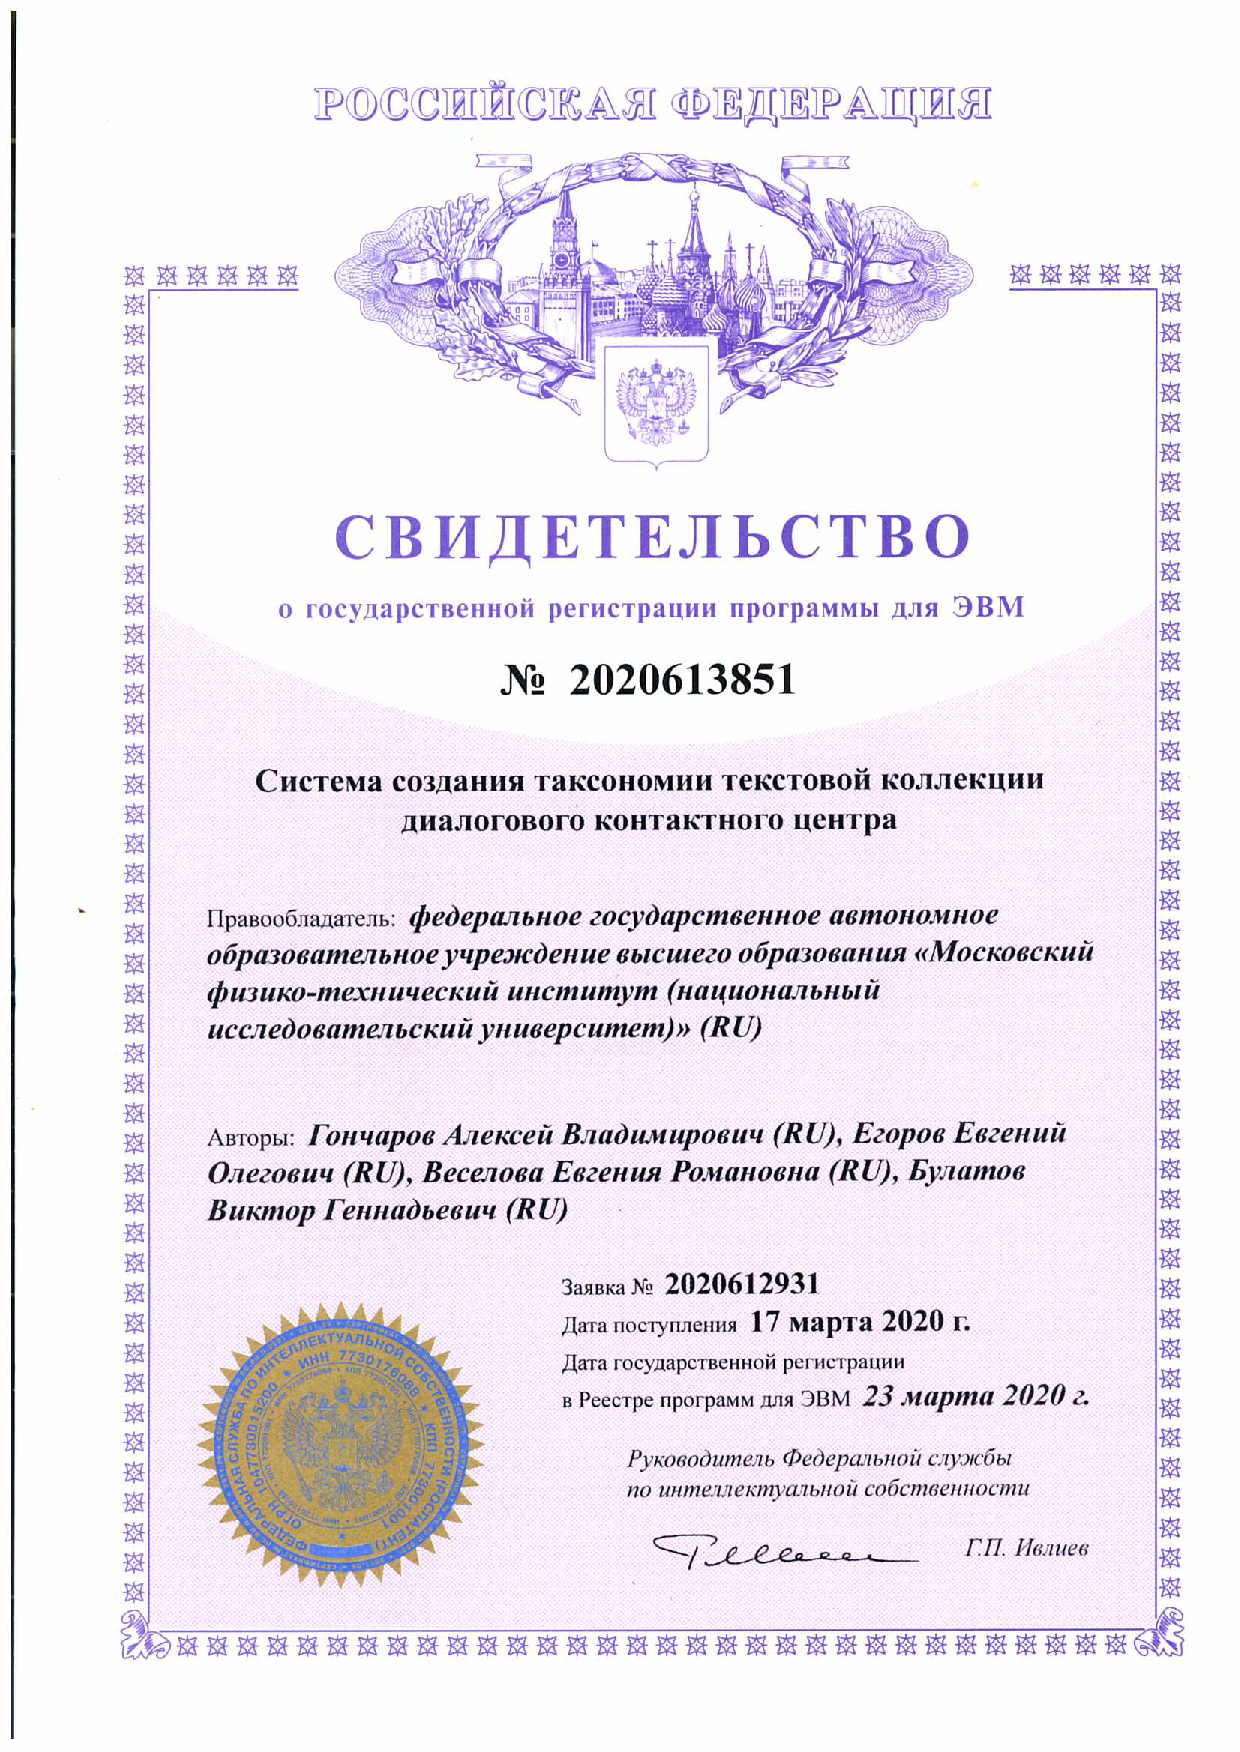
\includepdf[pages=-,scale=.8,offset=0 -25,pagecommand={
    \chapter{Свидетельства о государственной регистрации программ}\label{app:A}
}]{Documents/Taxonomy_2020613851.pdf}
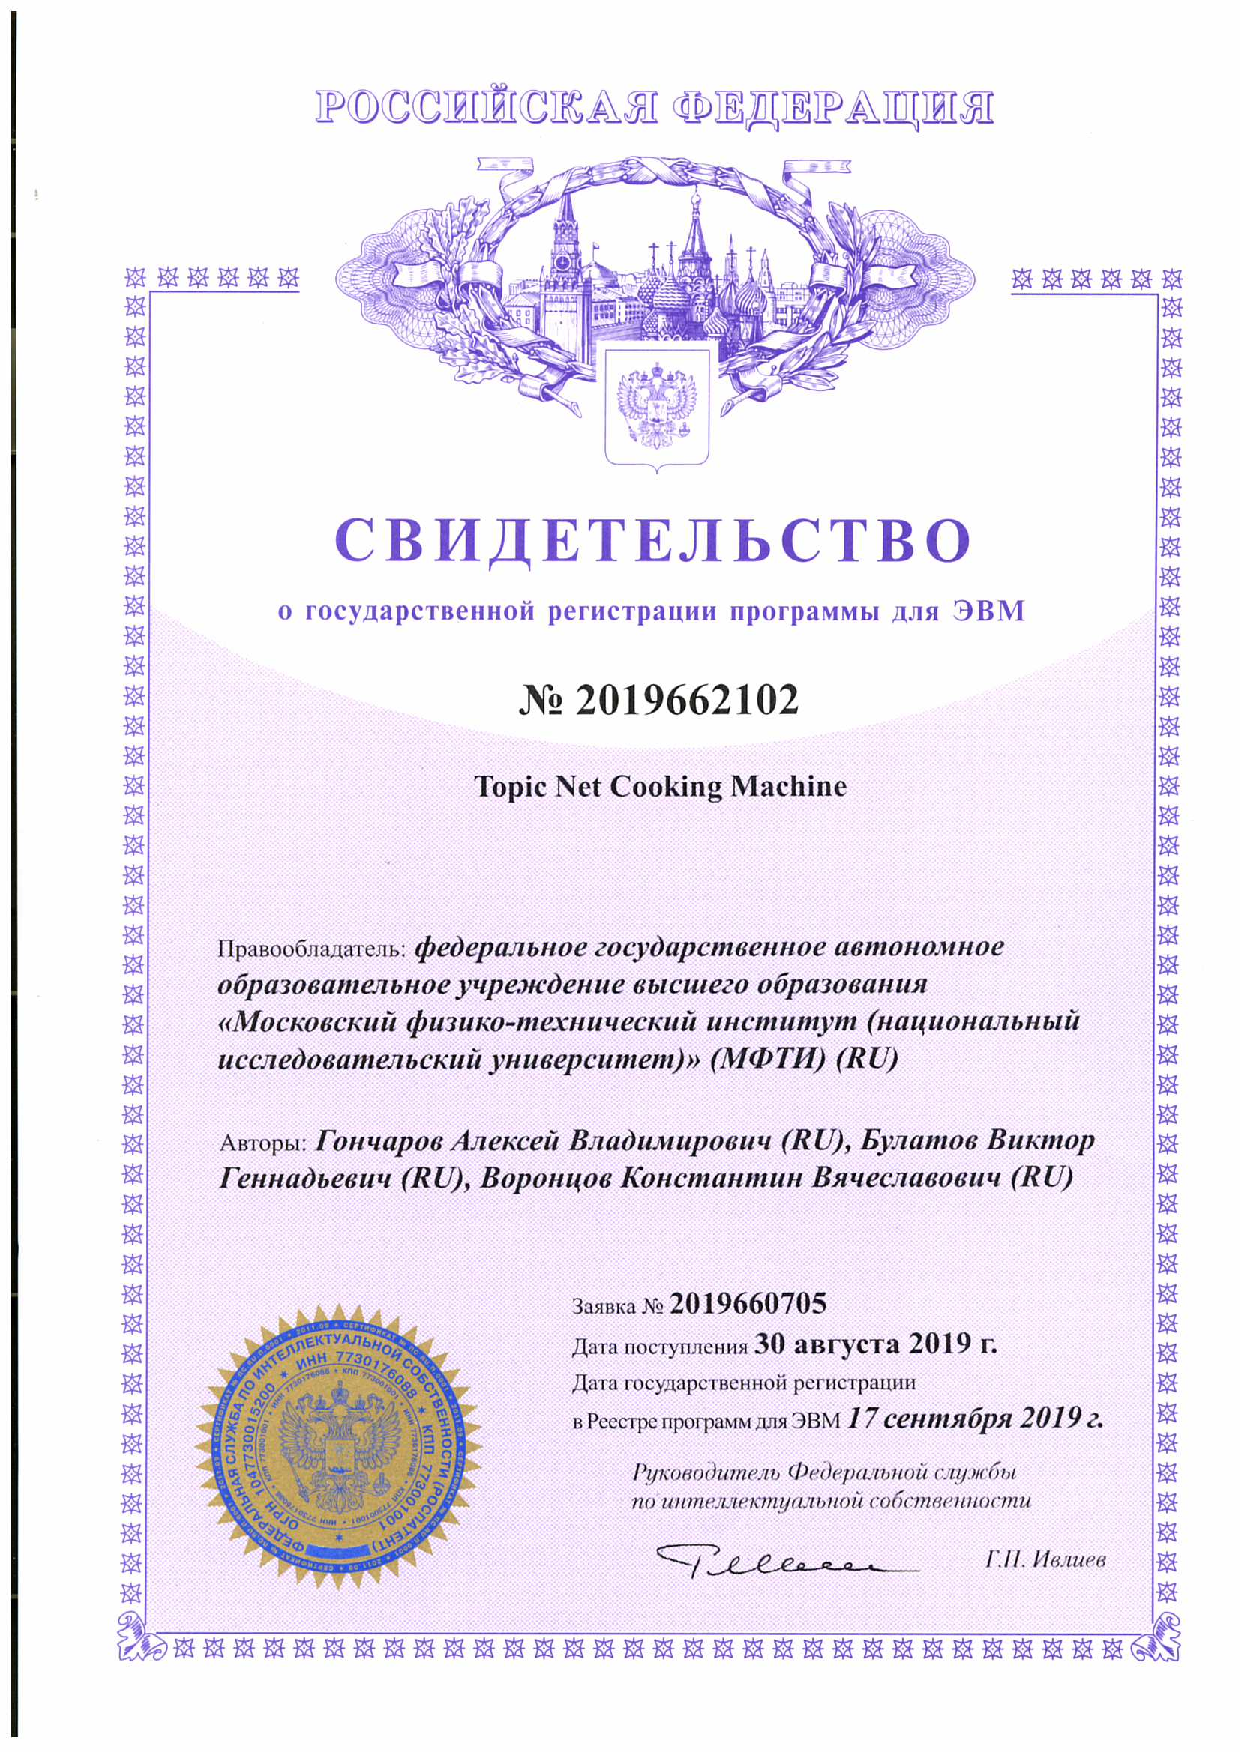
\includepdf[pages=-,scale=.8,offset=0 -25]{Documents/Topic Net Cooking Machine 2019662102.pdf}
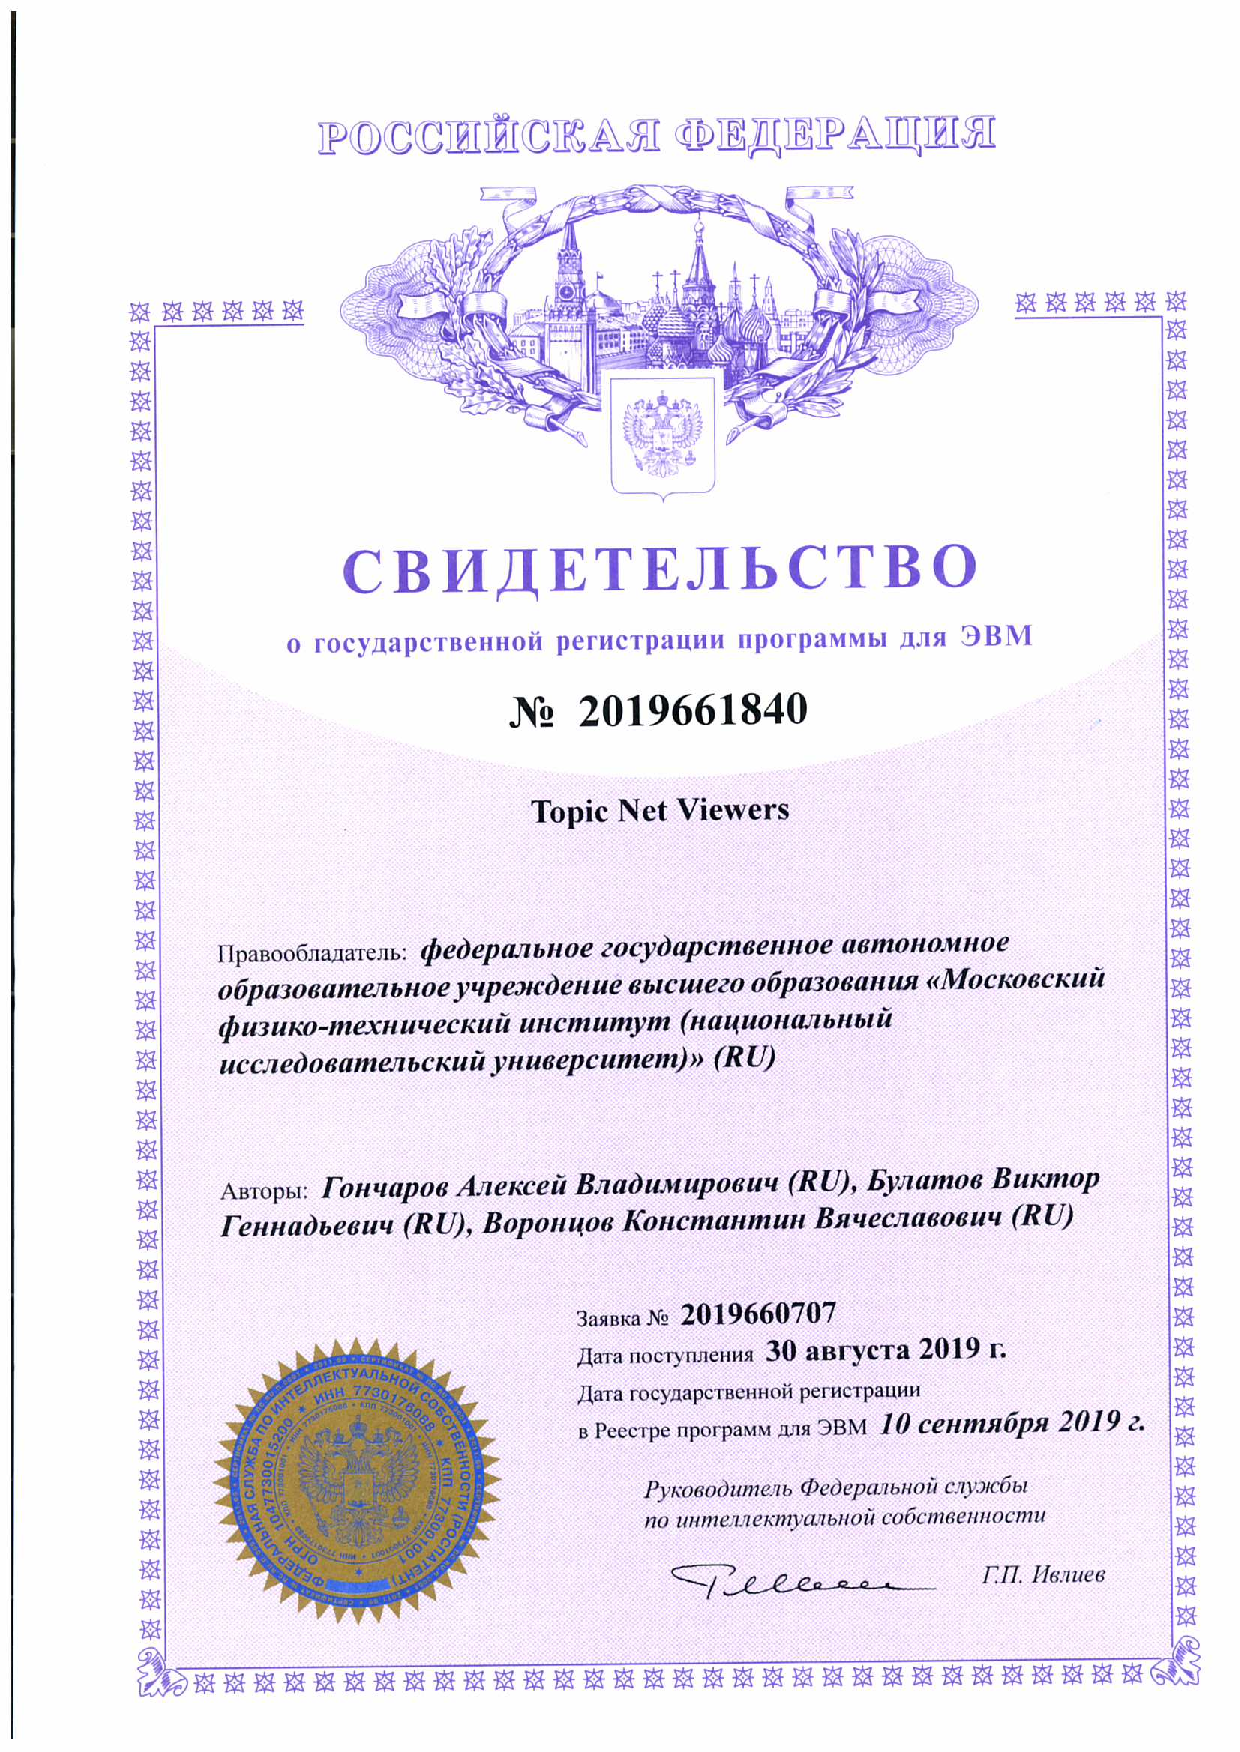
\includepdf[pages=-,scale=.8,offset=0 -25]{Documents/Topic Net Viewers 2019661840.pdf}
        % Приложения

\setcounter{totalappendix}{\value{chapter}} % Подсчёт количества приложений

\end{document}
